\documentclass[landscape,a0paper,fontscale=0.292]{baposter}

\usepackage[vlined]{algorithm2e}
\usepackage{times}
\usepackage{calc}
\usepackage{url}
\usepackage{graphicx}
\usepackage{amsmath}
\usepackage{amssymb}
\usepackage{relsize}
\usepackage{multirow}
\usepackage{booktabs}
\usepackage{tikz}
\usepackage{tikz-3dplot}
\usepackage{tikzpagenodes}
\usepackage{graphicx}
\usepackage{pgfplots}
\usepackage{multicol}
\usepackage[T1]{fontenc}
\usepackage{ae}
\usetikzlibrary{shapes,arrows,decorations.pathmorphing,backgrounds,positioning,fit,matrix}
\graphicspath{{images/}}

 %%%%%%%%%%%%%%%%%%%%%%%%%%%%%%%%%%%%%%%%%%%%%%%%%%%%%%%%%%%%%%%%%%%%%%%%%%%%%%%%
 %%%% Some math symbols used in the text
 %%%%%%%%%%%%%%%%%%%%%%%%%%%%%%%%%%%%%%%%%%%%%%%%%%%%%%%%%%%%%%%%%%%%%%%%%%%%%%%%
 % Format 
 \newcommand{\RotUP}[1]{\begin{sideways}#1\end{sideways}}


 %%%%%%%%%%%%%%%%%%%%%%%%%%%%%%%%%%%%%%%%%%%%%%%%%%%%%%%%%%%%%%%%%%%%%%%%%%%%%%%%
 % Multicol Settings
 %%%%%%%%%%%%%%%%%%%%%%%%%%%%%%%%%%%%%%%%%%%%%%%%%%%%%%%%%%%%%%%%%%%%%%%%%%%%%%%%
 \setlength{\columnsep}{0.7em}
 \setlength{\columnseprule}{0mm}


 %%%%%%%%%%%%%%%%%%%%%%%%%%%%%%%%%%%%%%%%%%%%%%%%%%%%%%%%%%%%%%%%%%%%%%%%%%%%%%%%
 % Save space in lists. Use this after the opening of the list
 %%%%%%%%%%%%%%%%%%%%%%%%%%%%%%%%%%%%%%%%%%%%%%%%%%%%%%%%%%%%%%%%%%%%%%%%%%%%%%%%
 \newcommand{\compresslist}{%
 \setlength{\itemsep}{1pt}%
 \setlength{\parskip}{0pt}%
 \setlength{\parsep}{0pt}%
 }


 %%%%%%%%%%%%%%%%%%%%%%%%%%%%%%%%%%%%%%%%%%%%%%%%%%%%%%%%%%%%%%%%%%%%%%%%%%%%%%
 % Formating
 \newcommand{\Matrix}[1]{\begin{bmatrix} #1 \end{bmatrix}}
 \newcommand{\Vector}[1]{\begin{pmatrix} #1 \end{pmatrix}}

 \newcommand*{\norm}[1]{\mathopen\| #1 \mathclose\|}% use instead of $\|x\|$
 \newcommand*{\abs}[1]{\mathopen| #1 \mathclose|}% use instead of $\|x\|$
 \newcommand*{\normLR}[1]{\left\| #1 \right\|}% use instead of $\|x\|$

 \newcommand*{\SET}[1]  {\ensuremath{\mathcal{#1}}}
 \newcommand*{\FUN}[1]  {\ensuremath{\mathcal{#1}}}
 \newcommand*{\MAT}[1]  {\ensuremath{\boldsymbol{#1}}}
 \newcommand*{\VEC}[1]  {\ensuremath{\boldsymbol{#1}}}
 \newcommand*{\CONST}[1]{\ensuremath{\mathit{#1}}}

 \DeclareMathOperator*{\argmax}{arg\,max}
 \DeclareMathOperator*{\diag}{diag}
 \DeclareMathOperator*{\argmin}{arg\,min}
 \DeclareMathOperator*{\vectorize}{vec}
 \DeclareMathOperator*{\reshape}{reshape}

 %-----------------------------------------------------------------------------
 % Differentiation
 \newcommand*{\Nabla}[1]{\nabla_{\!#1}}

 \renewcommand*{\d}{\mathrm{d}}
 \newcommand*{\dd}{\partial}

 \newcommand*{\At}[2]{\ensuremath{\left.#1\right|_{#2}}}
 \newcommand*{\AtZero}[1]{\At{#1}{\pp=\VEC 0}}

 \newcommand*{\diffp}[2]{\ensuremath{\frac{\dd #1}{\dd #2}}}
 \newcommand*{\diffpp}[3]{\ensuremath{\frac{\dd^2 #1}{\dd #2 \dd #3}}}
 \newcommand*{\diffppp}[4]{\ensuremath{\frac{\dd^3 #1}{\dd #2 \dd #3 \dd #4}}}
 \newcommand*{\difff}[2]{\ensuremath{\frac{\d #1}{\d #2}}}
 \newcommand*{\diffff}[3]{\ensuremath{\frac{\d^2 #1}{\d #2 \d #3}}}
 \newcommand*{\difffp}[3]{\ensuremath{\frac{\dd\d #1}{\d #2 \dd #3}}}
 \newcommand*{\difffpp}[4]{\ensuremath{\frac{\dd^2\d #1}{\d #2 \dd #3 \dd #4}}}

 \newcommand*{\diffpAtZero}[2]{\ensuremath{\AtZero{\diffp{#1}{#2}}}}
 \newcommand*{\diffppAtZero}[3]{\ensuremath{\AtZero{\diffpp{#1}{#2}{#3}}}}
 \newcommand*{\difffAt}[3]{\ensuremath{\At{\difff{#1}{#2}}{#3}}}
 \newcommand*{\difffAtZero}[2]{\ensuremath{\AtZero{\difff{#1}{#2}}}}
 \newcommand*{\difffpAtZero}[3]{\ensuremath{\AtZero{\difffp{#1}{#2}{#3}}}}
 \newcommand*{\difffppAtZero}[4]{\ensuremath{\AtZero{\difffpp{#1}{#2}{#3}{#4}}}}

 %-----------------------------------------------------------------------------
 % Defined
 % How should the defined operator look like (:= or ^= ==)
 % (I want back my :=, it is so much better than ^= because (1) it has a
 % direction and (2) everyone here uses it.)
 %
 % Use :=
 %\newcommand*{\defined}{\ensuremath{\mathrel{\mathop{:}}=}}
 %\newcommand*{\definedRight}{\ensuremath{=\mathrel{\mathop{:}}}}
 % Use ^=
 \newcommand*{\defined}{\ensuremath{\triangleq}}
 \newcommand*{\definedRight}{\ensuremath{\triangleq}}
 % Use = with three bars
 %\newcommand*{\defined}{\ensuremath{?}}
 %\newcommand*{\definedRight}{\ensuremath{?}}

 %%%%%%%%%%%%%%%%%%%%%%%%%%%%%%%%%%%%%%%%%%%%%%%%%%%%%%%%%%%%%%%%%%%%%%%%%%%%%%
 % Symbols used in the paper

 %-----------------------------------------------------------------------------
 % The Methods
 \newcommand*{\ICIA}{\emph{ICIA}}
 \newcommand*{\CoDe}{\emph{CoDe}}
 \newcommand*{\LinCoDe}{\emph{LinCoDe}}
 \newcommand*{\CoNe}{\emph{CoNe}}
 \newcommand*{\CoLiNe}{\emph{CoLiNe}}
 \newcommand*{\LinCoLiNe}{\emph{LinCoLiNe}}

 % inter eye distance
 \newcommand*{\ied}{IED}

 %-----------------------------------------------------------------------------
 % Koerper
 %%\newcommand*{\RR}{\mathbb{R}}
 %\newcommand*{\RR}{{I\hspace{-3.5pt}R}}
 %\newcommand*{\RR}{{\mathrm{I\hspace{-2.7pt}R}}}

 \font\dsfnt=dsrom12

 \DeclareSymbolFont{nark}{U}{dsrom}{m}{n}
 \DeclareMathSymbol{\NN}{\dsfnt}{nark}{`N}
 \DeclareMathSymbol{\RR}{\dsfnt}{nark}{`R}
 \DeclareMathSymbol{\ZZ}{\dsfnt}{nark}{`Z}

 %-----------------------------------------------------------------------------
 % Domains
 \newcommand*{\D}{\mathcal{D}}
 \newcommand*{\I}{\mathcal{I}}

 %-----------------------------------------------------------------------------
 % Texture coordinates
 \newcommand*{\rr}{\VEC{r}}

 %-----------------------------------------------------------------------------
 % Parameters
 \newcommand*{\pt}{\VEC{\tau}}
 \newcommand*{\pr}{\VEC{\rho}}
 \newcommand*{\pp}{\VEC{p}}
 \newcommand*{\qq}{\VEC{q}}
 \newcommand*{\xx}{\VEC{x}}
 \newcommand*{\deltaq}{\Delta \qq}
 \newcommand*{\deltap}{\Delta \pp}
 \newcommand*{\zz}{\VEC{z}}
 \newcommand*{\pa}{\VEC{\alpha}}
 \newcommand*{\qa}{\VEC{\alpha}}
 \newcommand*{\pb}{\VEC{\beta}}

 %-----------------------------------------------------------------------------
 % Optimal appearance parameters
 \newcommand*{\pbh}[1]{\ensuremath{\hat{\pb}({#1})}}

 %-----------------------------------------------------------------------------
 % Warp basis
 \newcommand*{\M}[1]{\ensuremath{M({#1})}}
 \newcommand*{\LL}[1]{\ensuremath{L({#1})}}

 %-----------------------------------------------------------------------------
 % Matrices of the texture model
 \newcommand*{\AM}[1]{\ensuremath{\Lambda(#1)}}               % Lambda(beta) 
 \newcommand*{\AMr}[2]{\ensuremath{\Lambda(#1; #2)}}        % Lambda(r, beta)

 \newcommand*{\As}{A}         % Continuous Basis symbol
 \newcommand*{\afs}{a}        % Continuous mean symbol
 \newcommand*{\A}[1]{\As(#1)}         % Continuous Basis
 \newcommand*{\af}[1]{\afs(#1)}        % Continuous mean


 %-----------------------------------------------------------------------------
 % Matrices of the shape model
 \newcommand*{\MU}{\VEC{\mu}}
 \newcommand*{\MM}{\MAT{M}}

 %-----------------------------------------------------------------------------
 %% The project out matrix and operator
 \newcommand*{\INT}{\MAT{P}}
 \newcommand*{\INTf}{P}

 %-----------------------------------------------------------------------------
 % The identity matrix
 \newcommand*{\EYEtwo}{\Matrix{1 & 0\\0&1}}
 \newcommand*{\EYE}{\MAT E}
 \newcommand*{\EYEf}{E}

 % Wether to use subscripts or brackets for some function arguments
 % can be decided by commenting out the corresponding functions underneath
 %-----------------------------------------------------------------------------
 % Mapping
 \newcommand*{\Cs}[1]{\ensuremath{C^{#1}}} % C symbol
 \newcommand*{\C}[2]{\ensuremath{C^{#1}(#2)}} % Use C with brackets

 %-----------------------------------------------------------------------------
 % Objective function
 \newcommand*{\Fs}{\ensuremath{F}}              % F symbol
 \newcommand*{\F}[1]{\ensuremath{\Fs(#1)}}       % Use F with brackets    F(q)

 %-----------------------------------------------------------------------------
 % Approximated objective functions
 \newcommand*{\FFs}{\tilde{F}}                     % ~F symbol
 \newcommand*{\FF}[1]{\ensuremath{\FFs(#1)}}       % Use ~F with brackets    F(q)

 %-----------------------------------------------------------------------------
 % residual function
 \newcommand*{\es}{\ensuremath{f}}              % R symbol

 \newcommand*{\e}[1]{\ensuremath{\es(#1)}}         % R(q)
 \newcommand*{\er}[2]{\ensuremath{\es(#1; #2)}}    % R(r; q)

 %-----------------------------------------------------------------------------
 % Approximated residual functions
 \newcommand*{\ees}{\tilde{f}}                       % ~R symbol
 \newcommand*{\ee}[1]{\ensuremath{\ees(#1)}}       % ~R(q)
 \newcommand*{\eer}[2]{\ensuremath{\ees(#2; #1)}}  % ~R(r; q)

 %-----------------------------------------------------------------------------
 % Warps
 \newcommand*{\Vs}{\ensuremath{V}}
 \newcommand*{\VLins}{\ensuremath{\Vs^{\text{Ortho}}}}
 \newcommand{\VModels}{\ensuremath{\Vs^{\text{Model}}}}
 \newcommand*{\Ws}{\ensuremath{W}}

 \newcommand{\V}[1]{\ensuremath{\Vs(#1)}}
 \newcommand{\VModel}[1]{\ensuremath{\VModels(#1)}}
 \newcommand{\Vr}[2]{\ensuremath{\Vs(#1; #2)}}
 \newcommand{\VInvr}[2]{\ensuremath{\Vs^{-1}(#1; #2)}}
 \newcommand{\VrLin}[2]{\ensuremath{\VLins(#1; #2)}}
 \newcommand{\W}[1]{\ensuremath{\Ws(#1)}}
 \newcommand{\Winv}[1]{\ensuremath{\Ws^{-1}(#1)}}
 \newcommand{\Wr}[2]{\ensuremath{\Ws(#1; #2)}}

\definecolor{dtugrey}{cmyk}{0,0,0,0.56}
\definecolor{dtured}{RGB}{153,0,0}
\definecolor{dturedcmyk}{cmyk}{0,0.91,0.72,0.23}
%%%%%%%%%%%%%%%%%%%%%%%%%%%%%%%%%%%%%%%%%%%%%%%%%%%%%%%%%%%%%%%%%%%%%%%%%%%%%
%% Begin of Document
%%%%%%%%%%%%%%%%%%%%%%%%%%%%%%%%%%%%%%%%%%%%%%%%%%%%%%%%%%%%%%%%%%%%%%%%%%%%%
\begin{document}
%%%%%%%%%%%%%%%%%%%%%%%%%%%%%%%%%%%%%%%%%%%%%%%%%%%%%%%%%%%%%%%%%%%%%%%%%%%%%
%% Here starts the poster
%%---------------------------------------------------------------------------
%% Format it to your taste with the options
%%%%%%%%%%%%%%%%%%%%%%%%%%%%%%%%%%%%%%%%%%%%%%%%%%%%%%%%%%%%%%%%%%%%%%%%%%%%%
\begin{poster}{
 % Show grid to help with alignment
 grid=false,
 % Column spacing
 colspacing=0.5em,
 % Color style
 headerColorOne=dtugrey!20,
 %cyan!50!white!90!black,
 borderColor=dturedcmyk!100,%cyan!30!white!90!black,
 % Format of textbox
 textborder=faded,
 % Format of text header
 headerborder=open,
 headershape=roundedright,
 headershade=plain,
 background=none,
 bgColorOne=cyan!10!white,
 headerheight=0.12\textheight,
 headerFontColor=black}
 % Eye Catcher
 {
      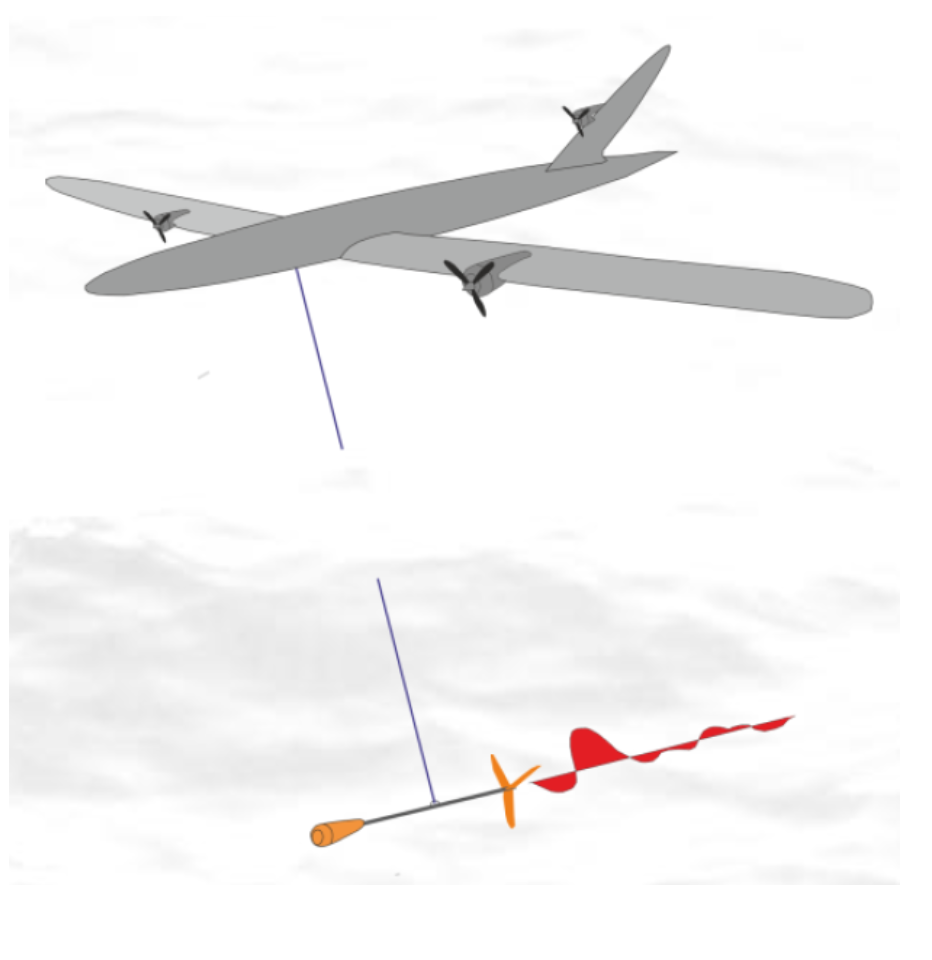
\includegraphics[width=0.1\linewidth]{figures/poster/pjd.png}
%      \includegraphics[width=0.1\linewidth]{figures/poster/.png}
%      \includegraphics[width=0.1\linewidth]{figures/poster/.png}
		%\raisebox{-12ex}{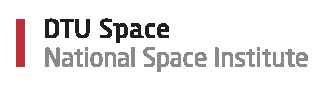
\includegraphics[width=0.15\linewidth]{../logos/tex_dtu_space_b_uk}}
 }
 % Title
 {\sc\Huge Poster session for 02901 Advanced Topics in Machine Learning}
 % Authors
 {Xiao Hu\\[0.5em]
 {\texttt{xiahaa@space.dtu.dk}}}
 % University logo
 {
  \begin{tabular}{r}
    
\includegraphics[height=0.08\textheight]{tex_dtu_logo}
  \end{tabular}
 }

%%%%%%%%%%%%%%%%%%%%%%%%%%%%%%%%%%%%%%%%%%%%%%%%%%%%%%%%%%%%%%%%%%%%%%%%%%%%%%
%%% Now define the boxes that make up the poster
%%%---------------------------------------------------------------------------
%%% Each box has a name and can be placed absolutely or relatively.
%%% The only inconvenience is that you can only specify a relative position 
%%% towards an already declared box. So if you have a box attached to the 
%%% bottom, one to the top and a third one which should be inbetween, you 
%%% have to specify the top and bottom boxes before you specify the middle 
%%% box.
%%%%%%%%%%%%%%%%%%%%%%%%%%%%%%%%%%%%%%%%%%%%%%%%%%%%%%%%%%%%%%%%%%%%%%%%%%%%%%

%%%%%%%%%%%%%%%%%%%%%%%%%%%%%%%%%%%%%%%%%%%%%%%%%%%%%%%%%%%%%%%%%%%%%%%%%%%%%%
  \headerbox{Project: UAV-QMS}{name=contribution,column=0,row=0,span=2}{
%%%%%%%%%%%%%%%%%%%%%%%%%%%%%%%%%%%%%%%%%%%%%%%%%%%%%%%%%%%%%%%%%%%%%%%%%%%%%%
	\setlength{\fboxrule}{0.0pt}
%	\begin{figure}
\framebox{\parbox{3.1in}{
		The UAV-QMS project aims to develop a cost-efficient and long range Unmanned Aerial Vehicle for high-Quality Magnetic Surveying. Due to the sensitivity of the surveying sensors, direct positioning the magnetic bird via traditional sensors like GPS is infeasible. Relative pose estimation using computer vision will be investigated in the project. The focus of the PhD thesis is to investigate:
		\begin{itemize}
			\item Pose estimation.
			\item Navigation.
		\end{itemize}
	}}
\framebox{\parbox{3.1in}{
	\centering
	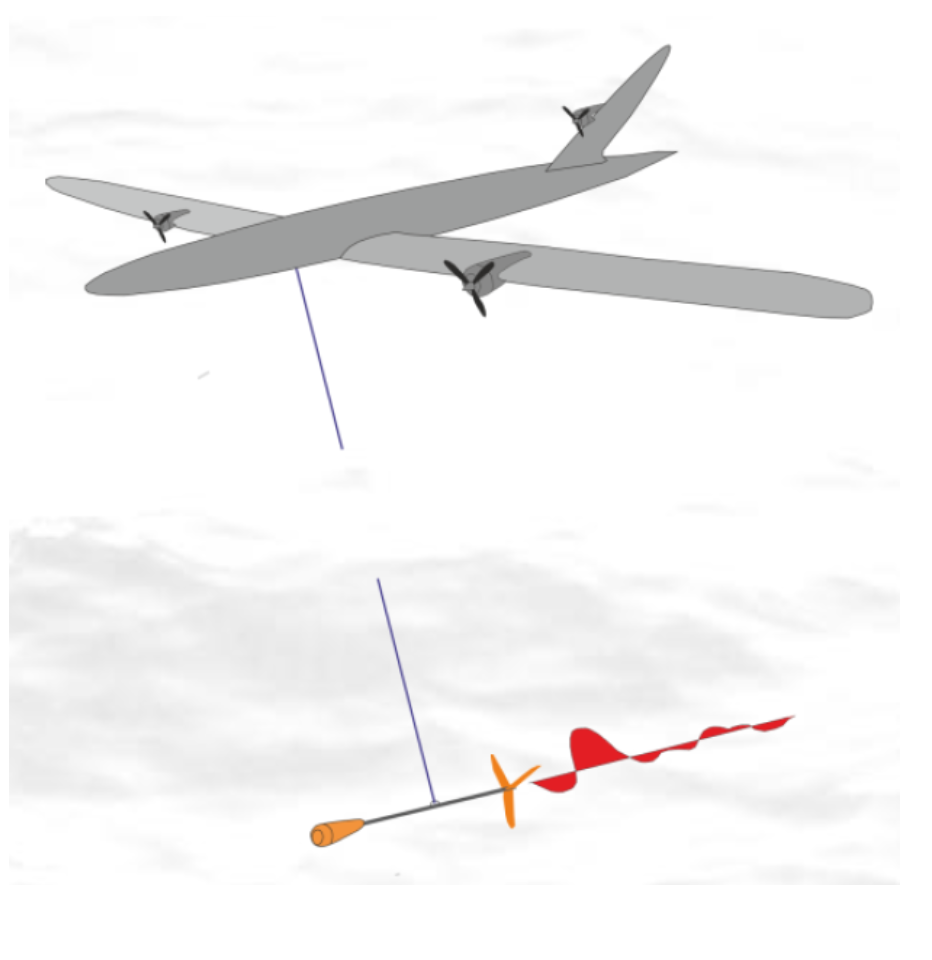
\includegraphics[width=0.3\textwidth]{figures/poster/pjd.png}
%	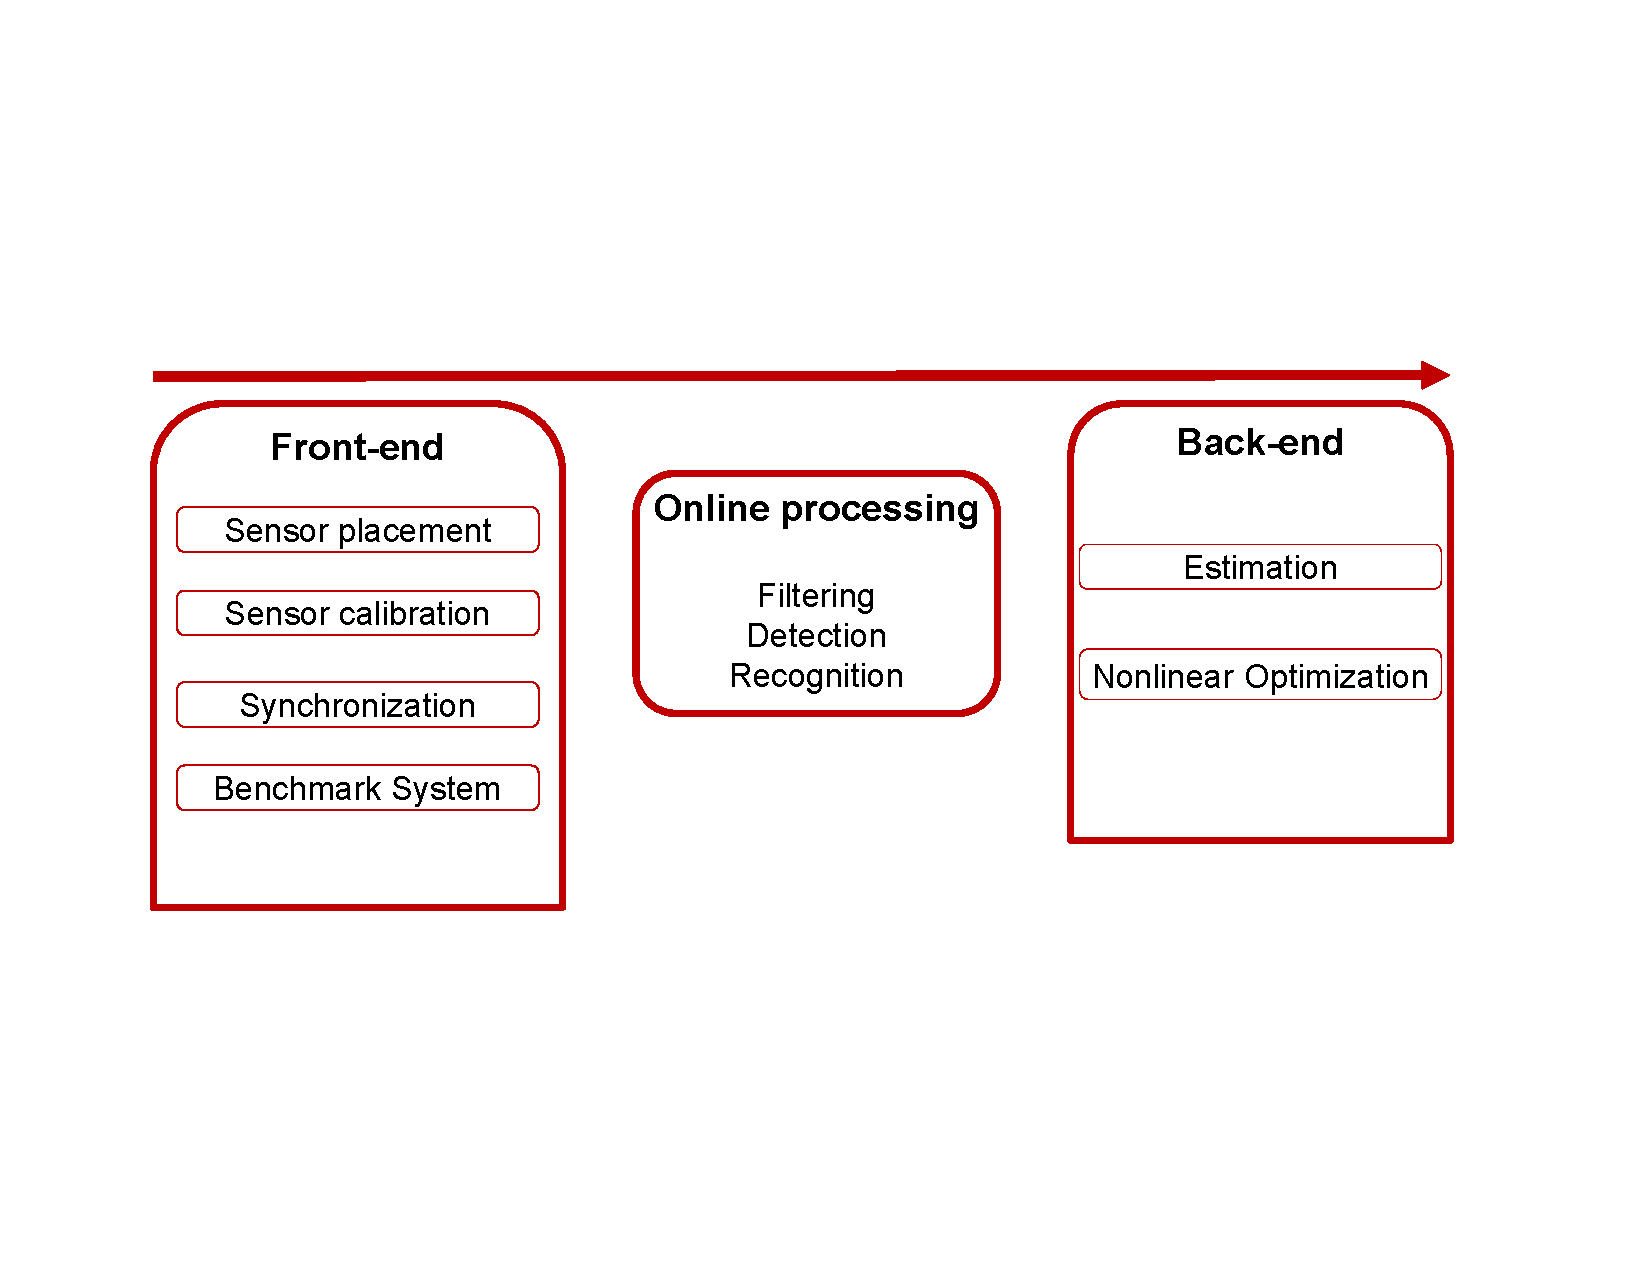
\includegraphics[width=0.3\textwidth]{figures/poster/system_bd}
}}
%	\end{figure}
}
%%%%%%%%%%%%%%%%%%%%%%%%%%%%%%%%%%%%%%%%%%%%%%%%%%%%%%%%%%%%%%%%%%%%%%%%%%%%%%
  \headerbox{Pose Estimation}{name=brc,column=0,row=0,span=2,below=contribution}{
  	  	\centering
\begin{tabular}{c@{\hspace{0.05em}}c@{\hspace{0.2em}}c@{\hspace{0.1em}}c@{\hspace{0.2em}}c@{\hspace{0.1em}}c@{\hspace{0.1em}}c}
	\multicolumn{2}{c}{\smaller Accurate Benchmark \& Pose Evaluation System} &\\[-0.2em]
	%   \multicolumn{2}{c}{\smaller Lucas-Kanade} &
	%   \multicolumn{2}{c}{\smaller Horn-Shunck} 
	  	\centering
	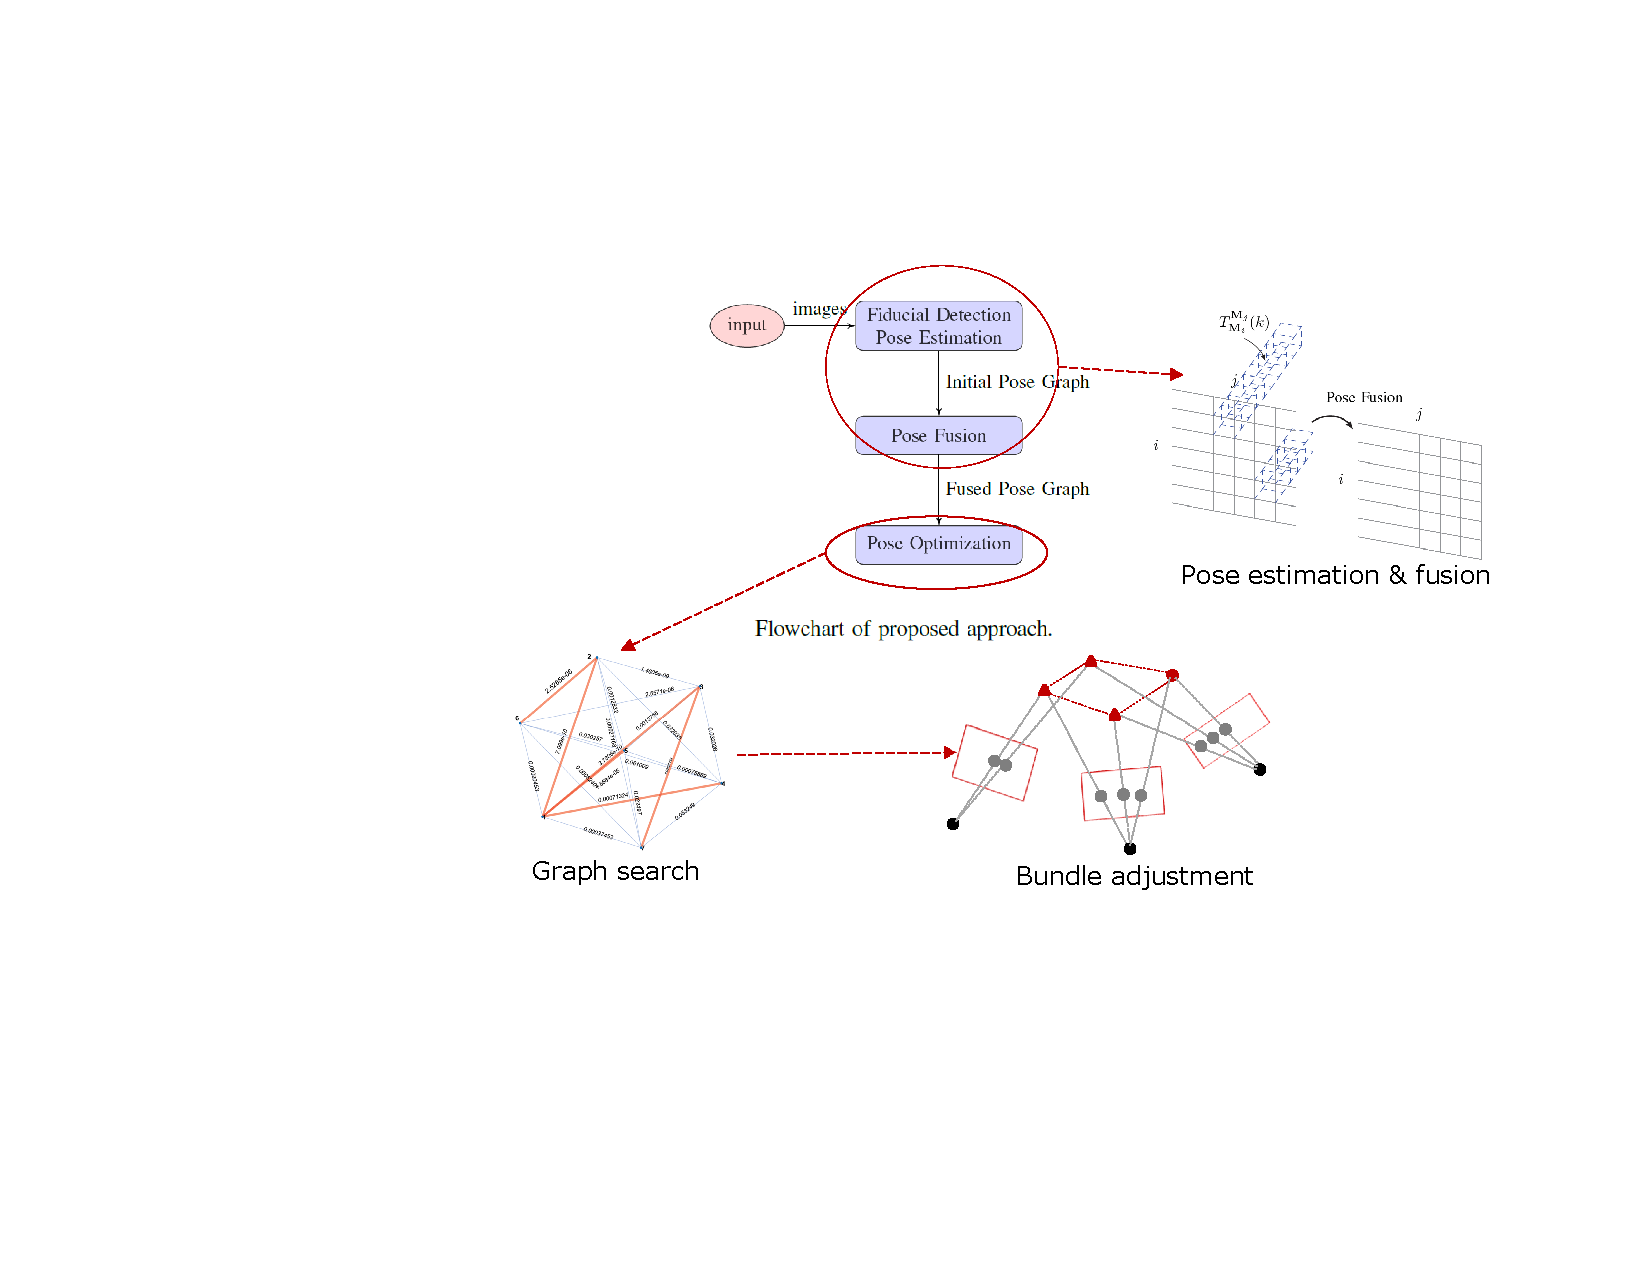
\includegraphics[width=0.4\linewidth]{figures/poster/ipinmm}&
	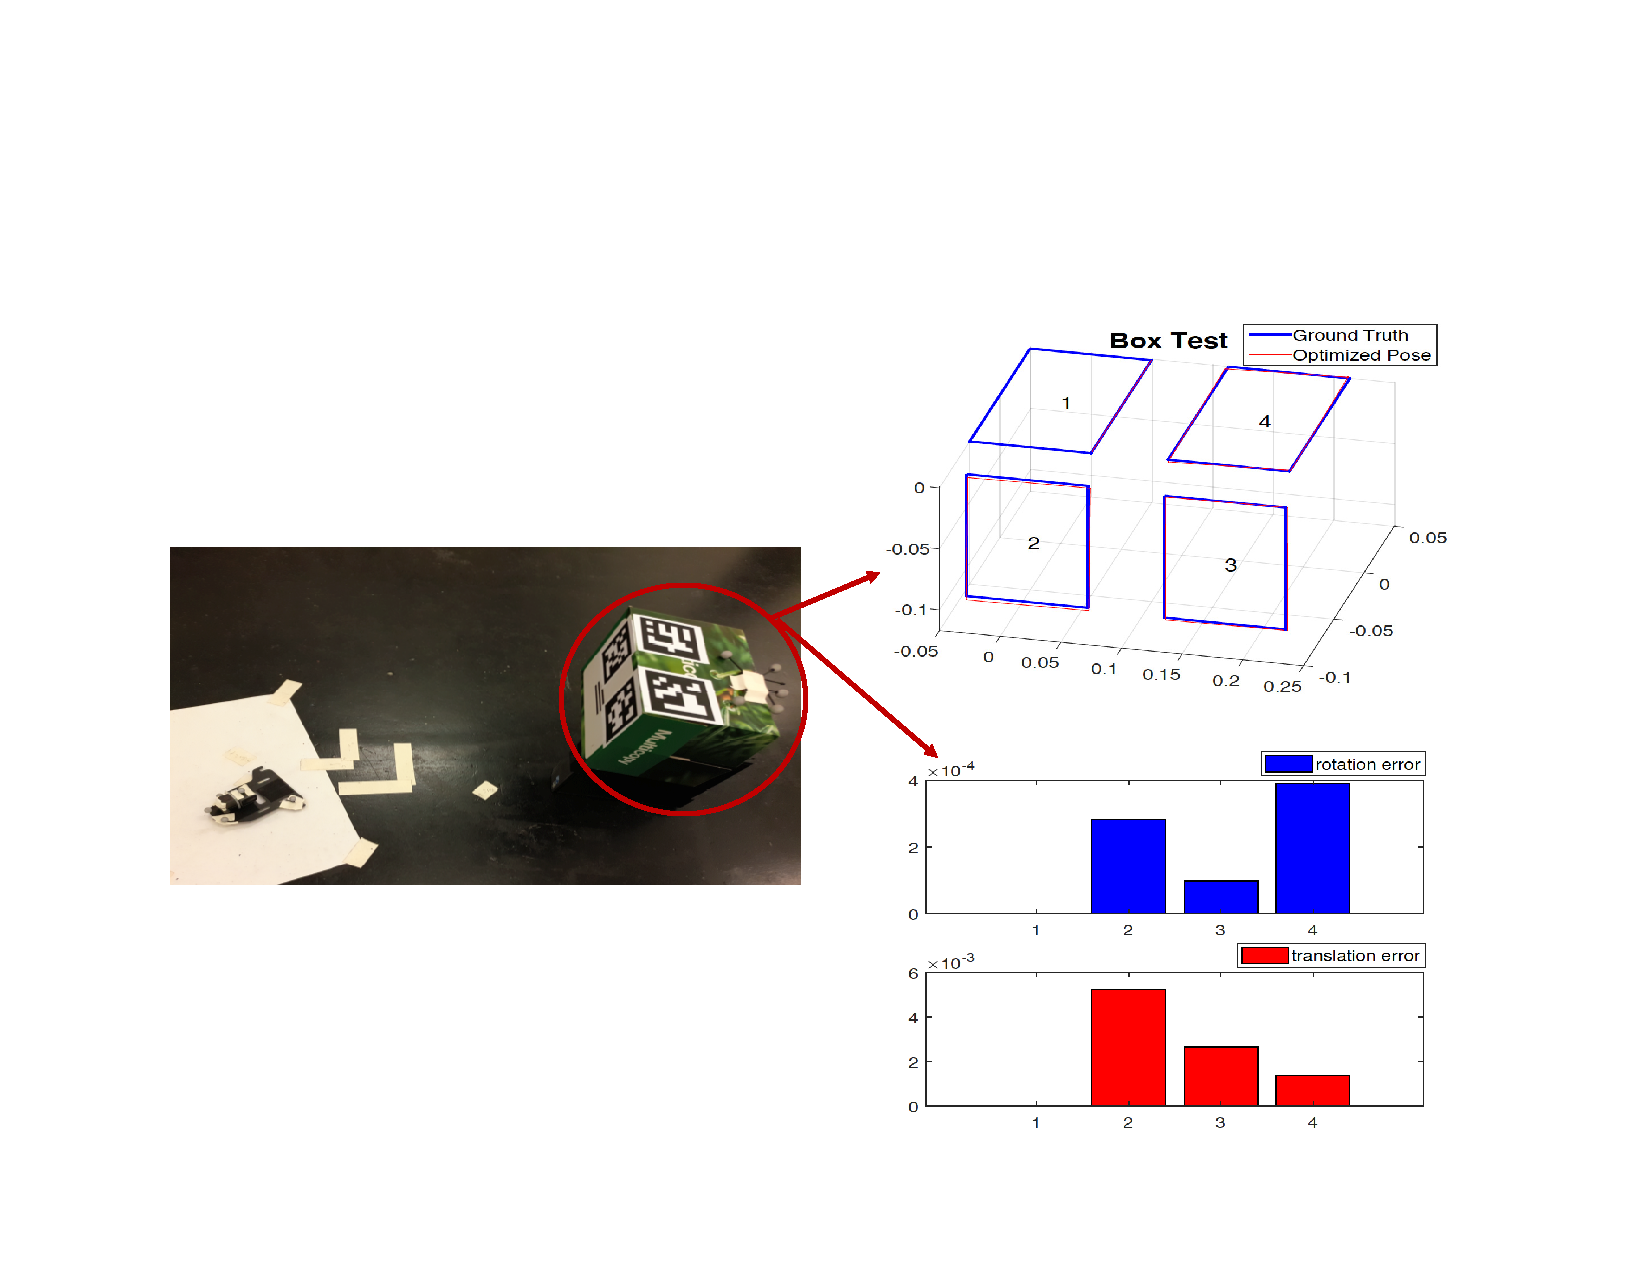
\includegraphics[width=0.4\linewidth]{figures/poster/res1}\\
	\smaller \textbf{Schematic Diagram} & \smaller \textbf{Mapping} \\[-0.1em]
	  	\centering
	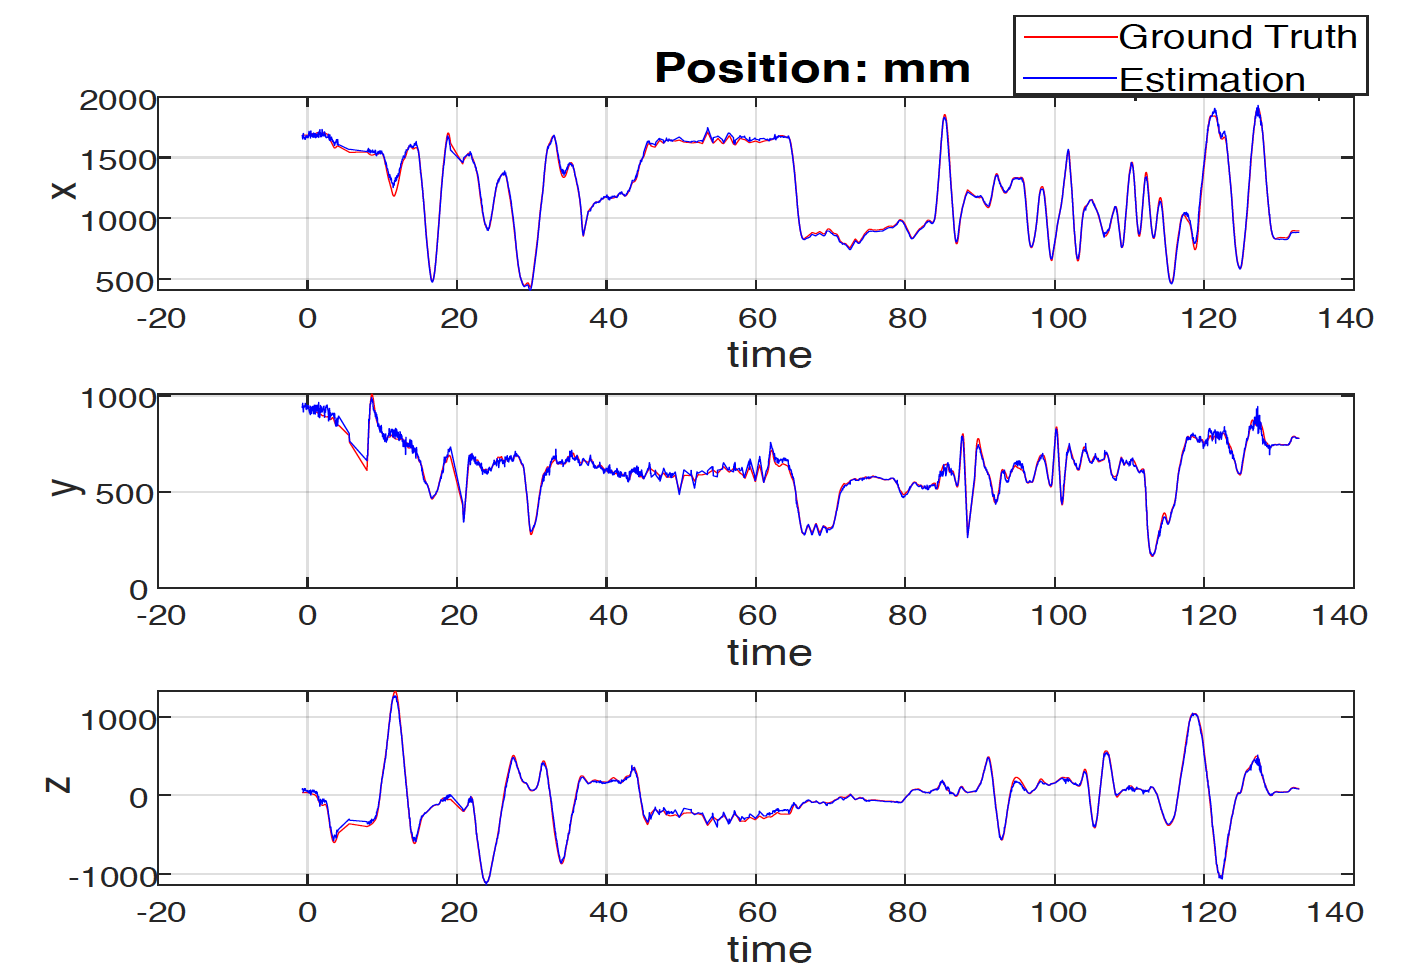
\includegraphics[width=0.4\linewidth]{figures/poster/poseest_t}&
	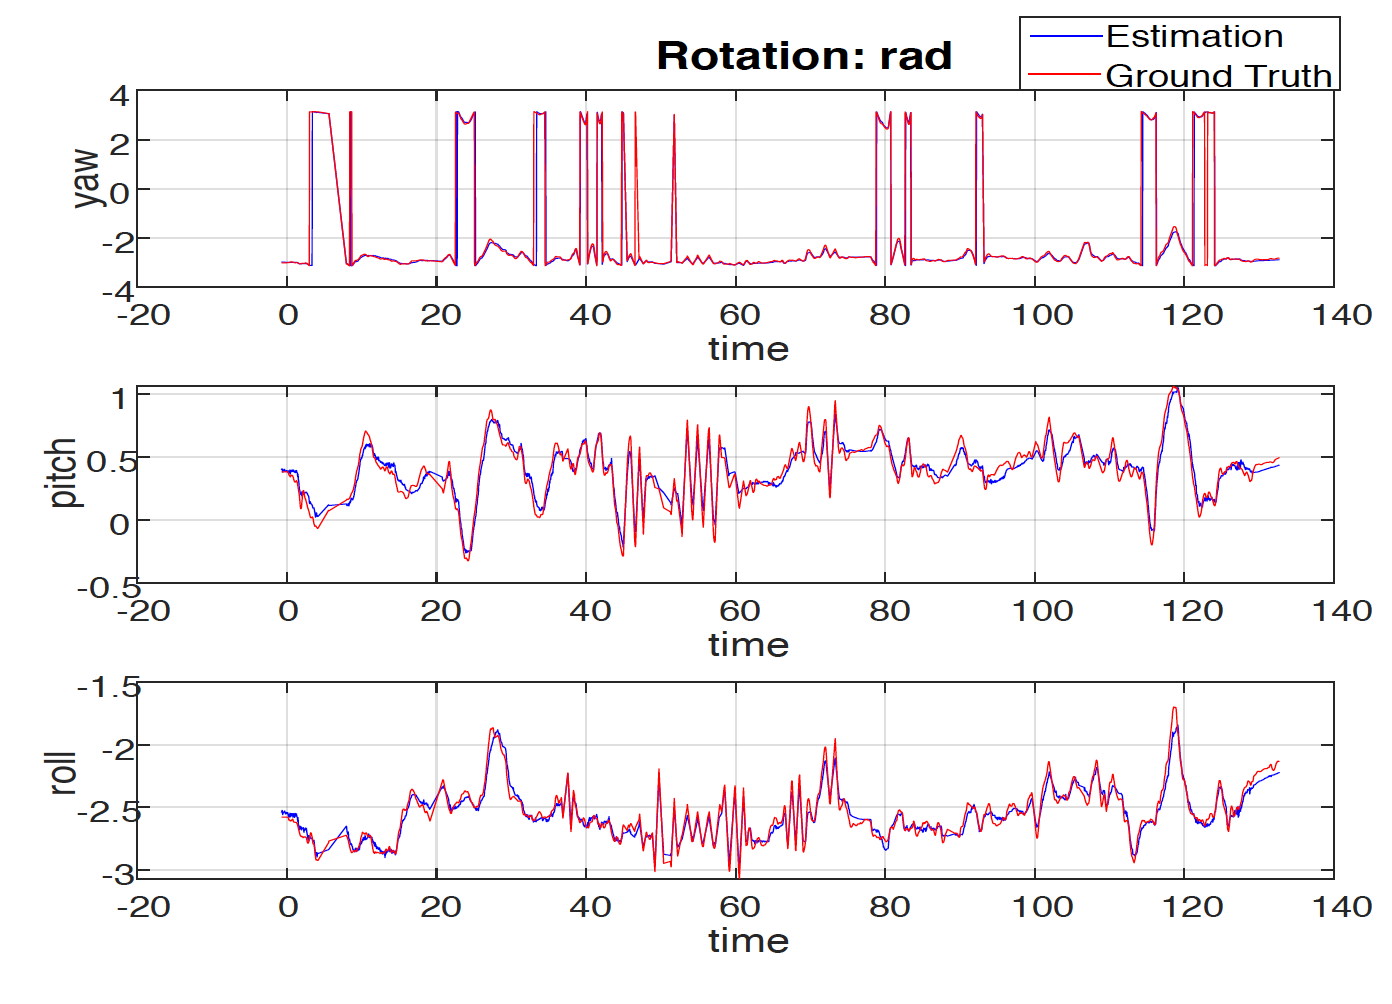
\includegraphics[width=0.4\linewidth]{figures/poster/poseest_r} \\
  \smaller \textbf{Translation Error} & \smaller \textbf{Rotation Error} 
	%
\end{tabular}  	
  	
  	
%  	
%  	
%	Schematic Diagram: \\
%  	\framebox{\parbox{3.1in}{
%  			\centering
%  			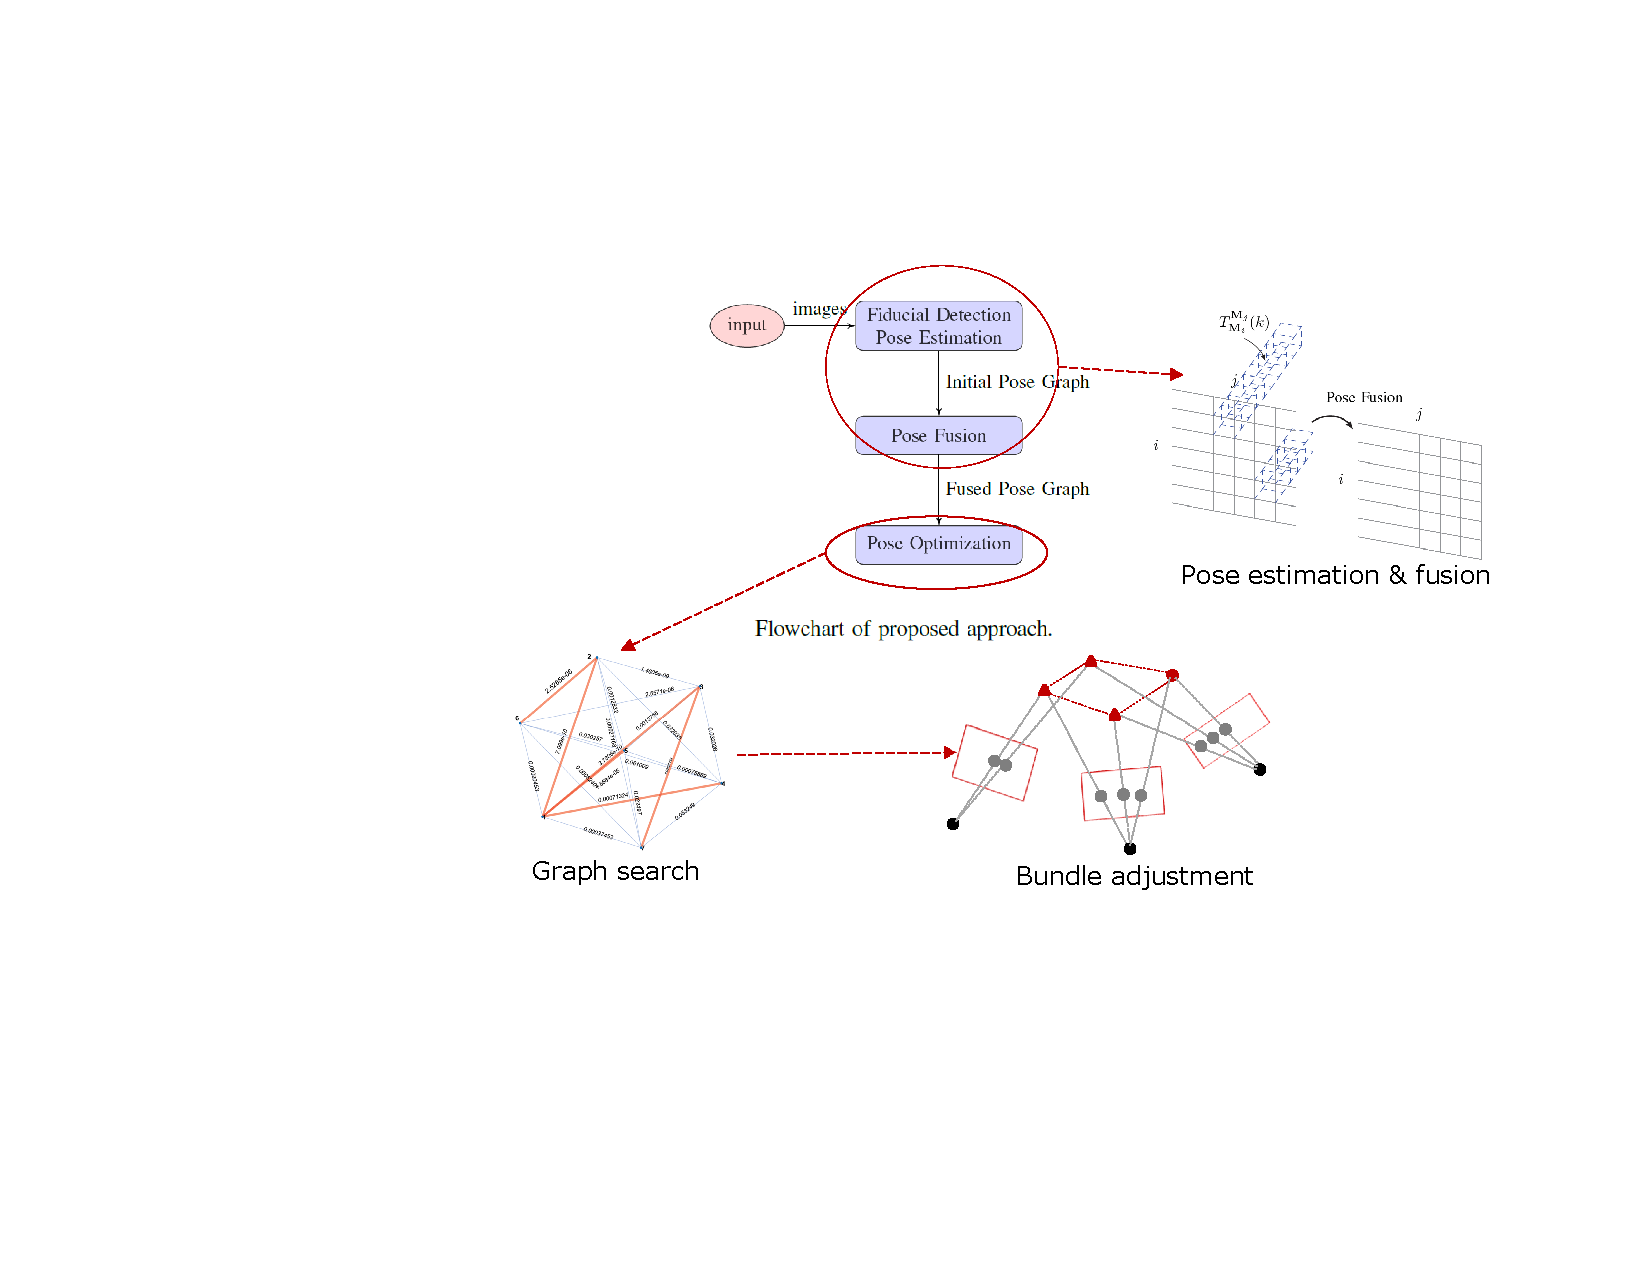
\includegraphics[width=0.5\textwidth]{figures/poster/ipinmm}
%  			%	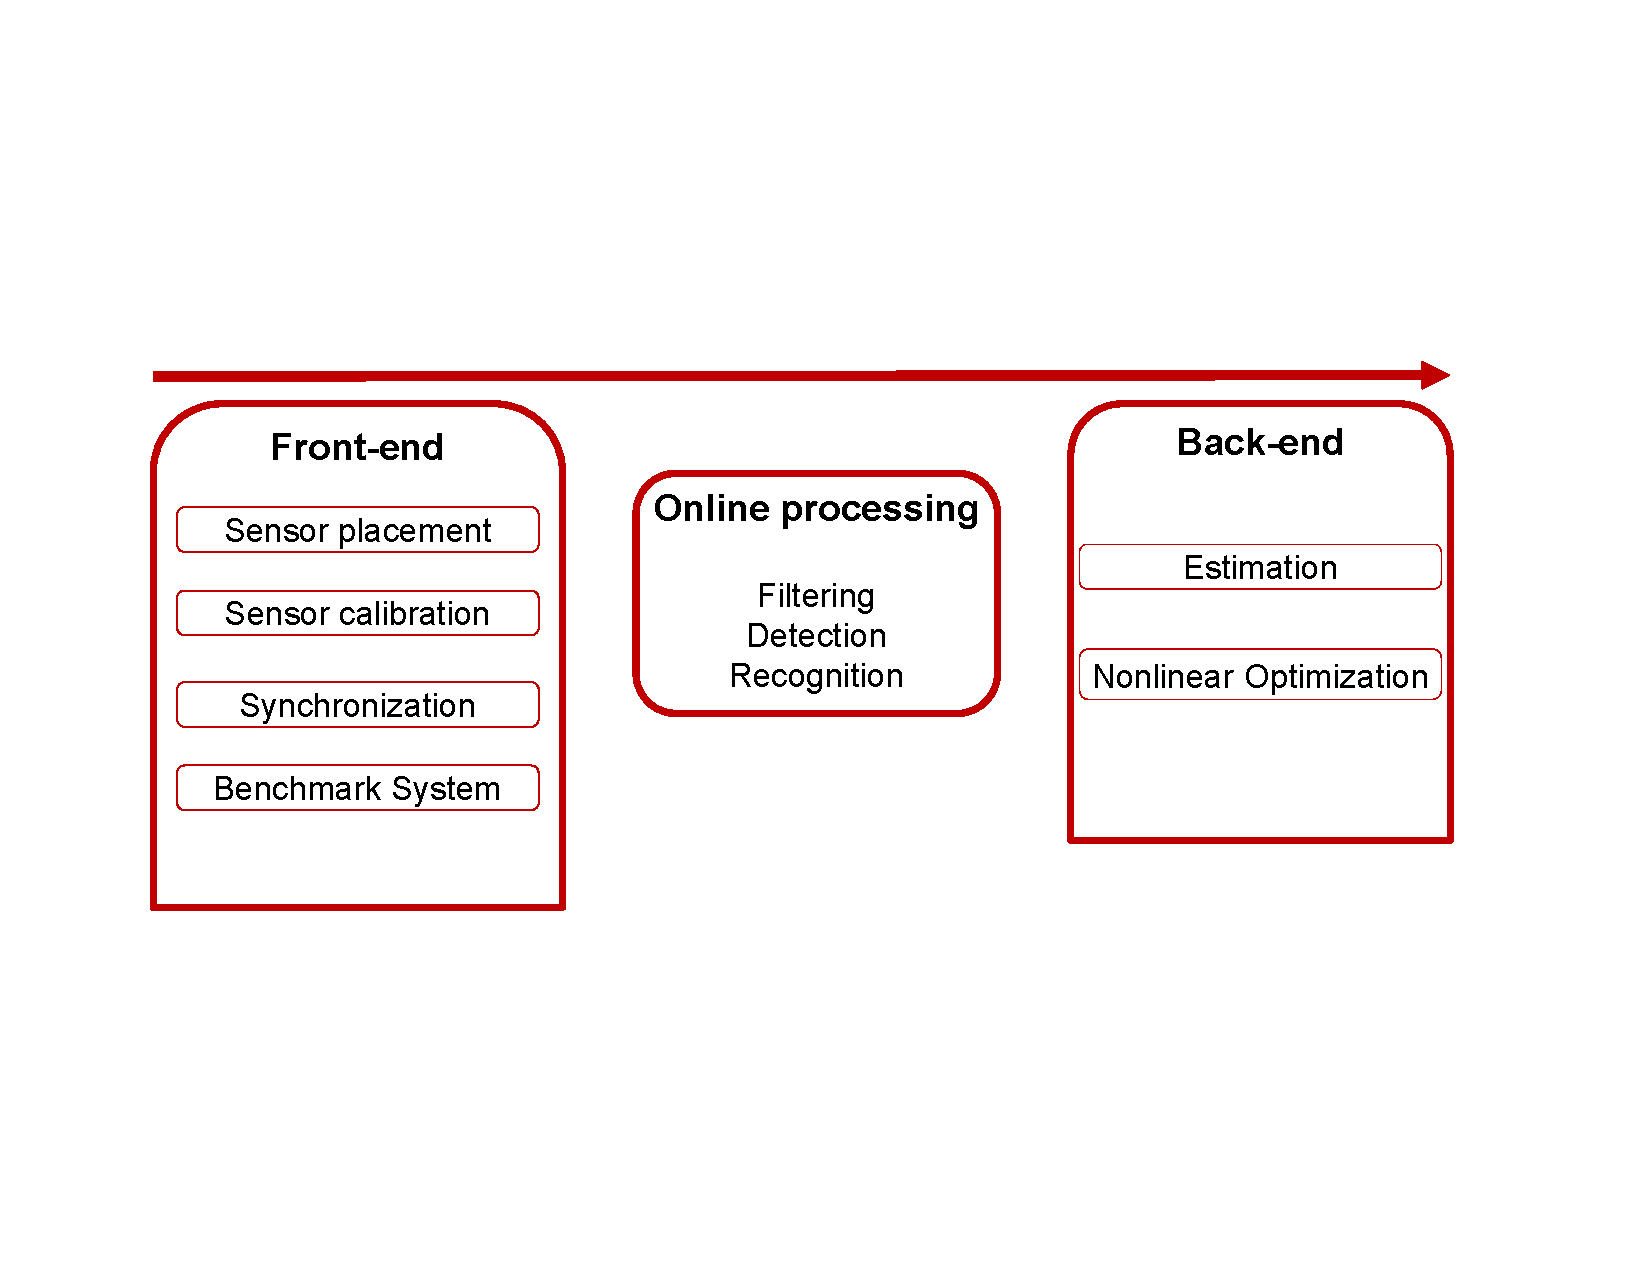
\includegraphics[width=0.3\textwidth]{figures/poster/system_bd}
%  	}}
%	\framebox{\parbox{3.1in}{
%	  		\centering
%	  		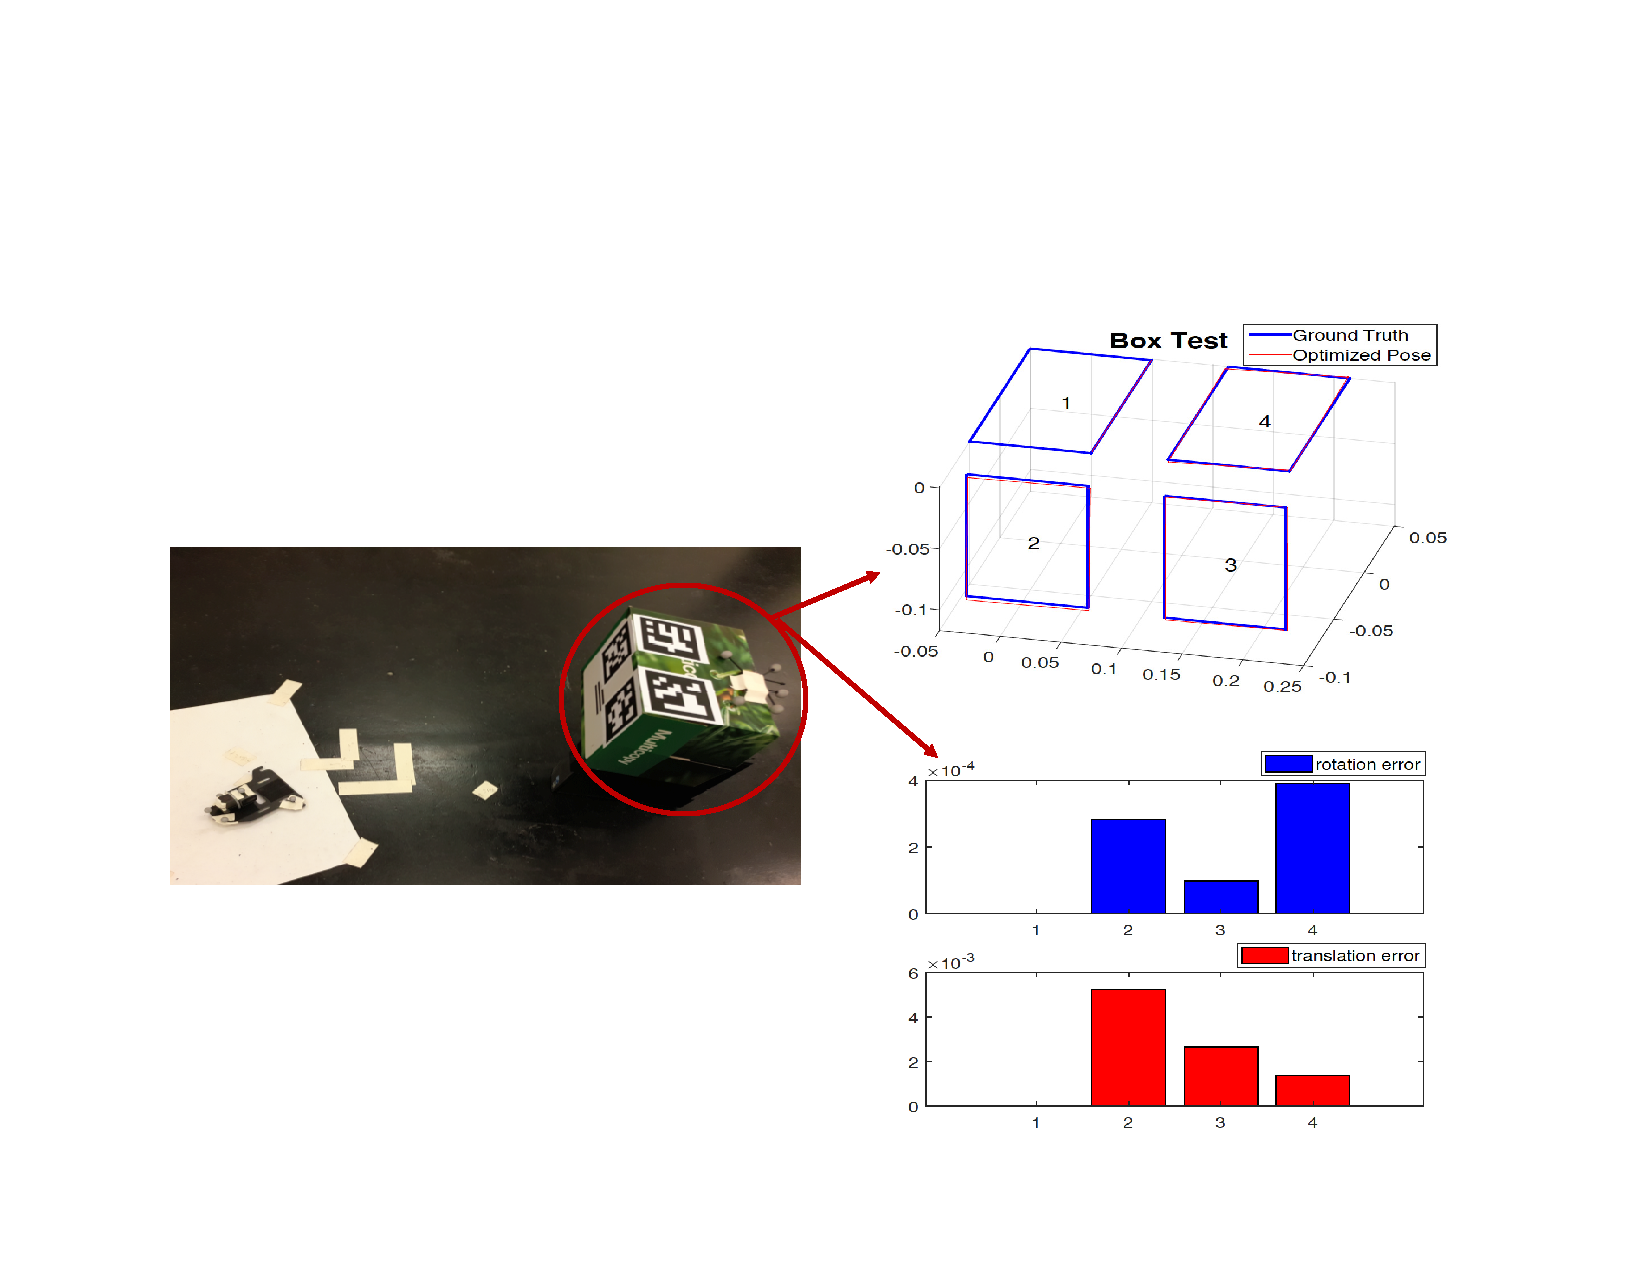
\includegraphics[width=0.5\textwidth]{figures/poster/res1}
%	  		%	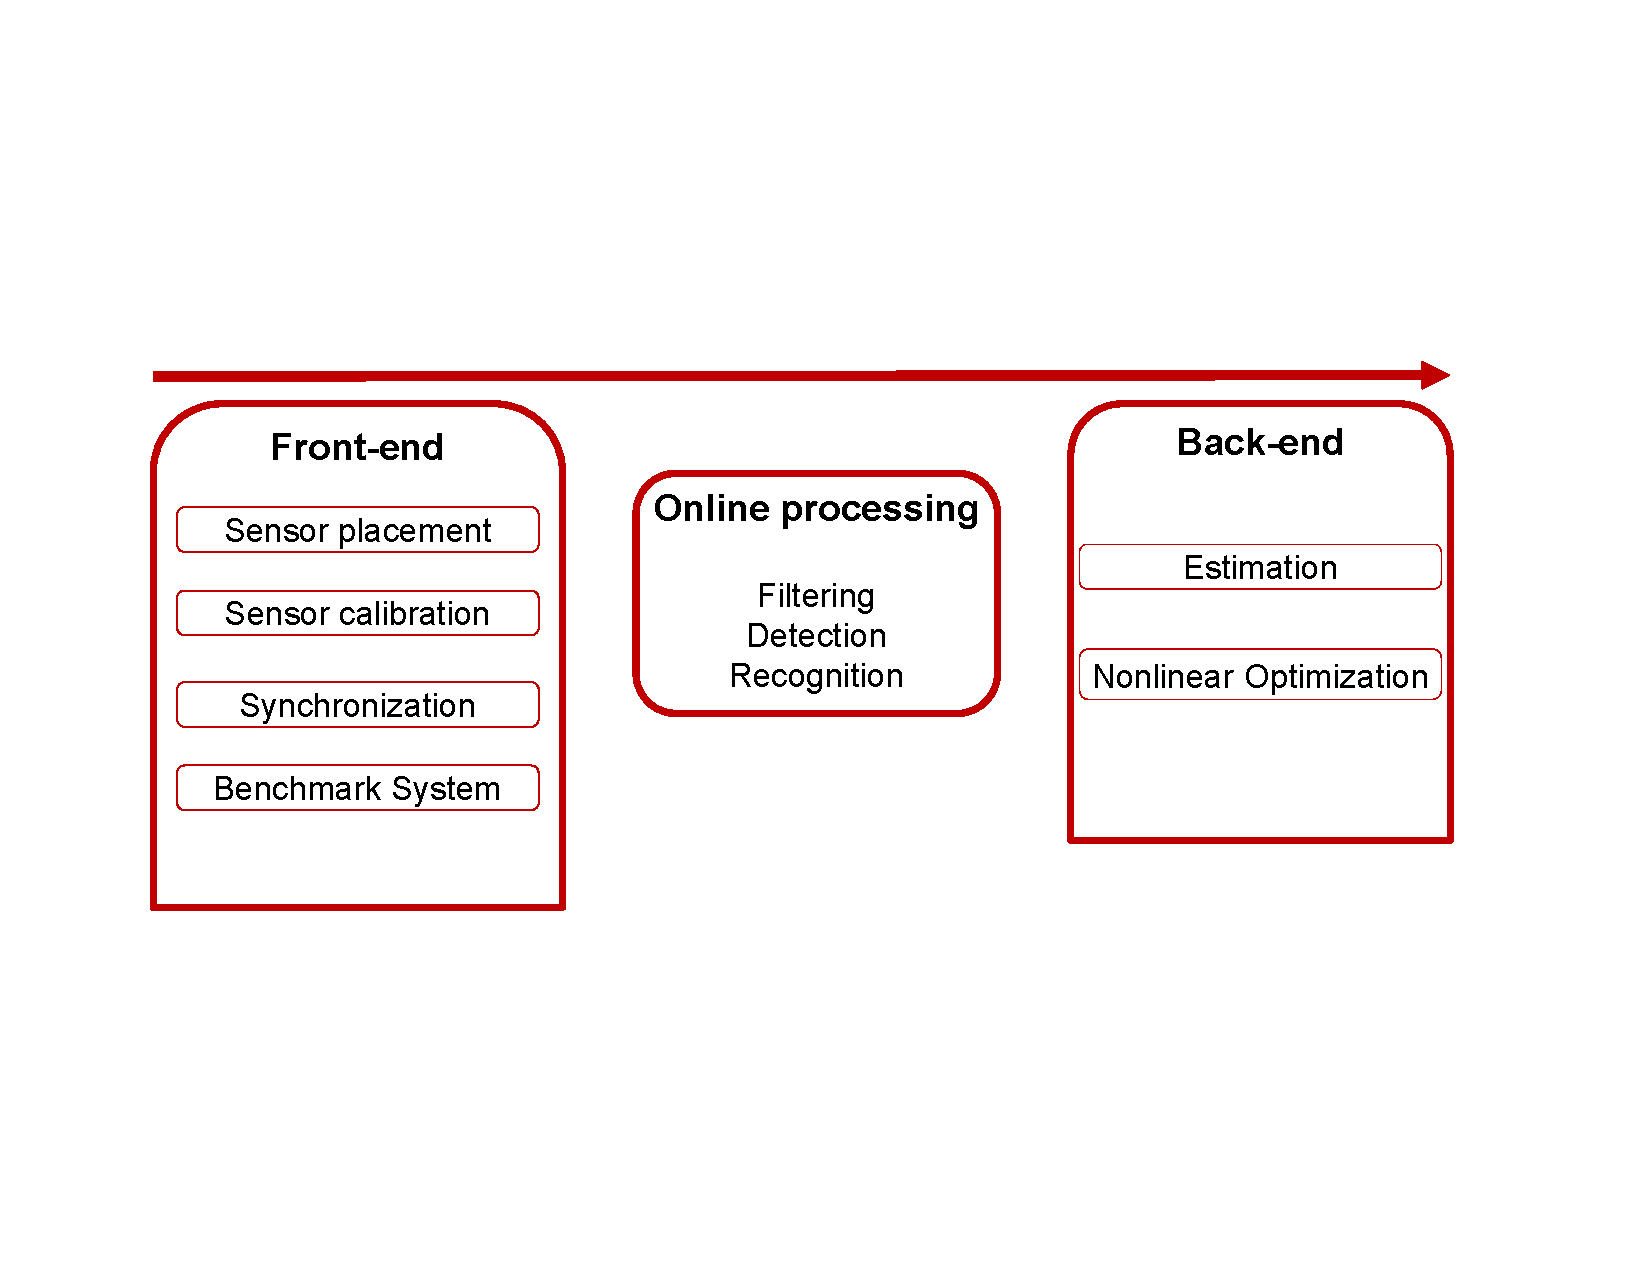
\includegraphics[width=0.3\textwidth]{figures/poster/system_bd}
%	}}
%  	\framebox{\parbox{3.1in}{
%		\centering
%		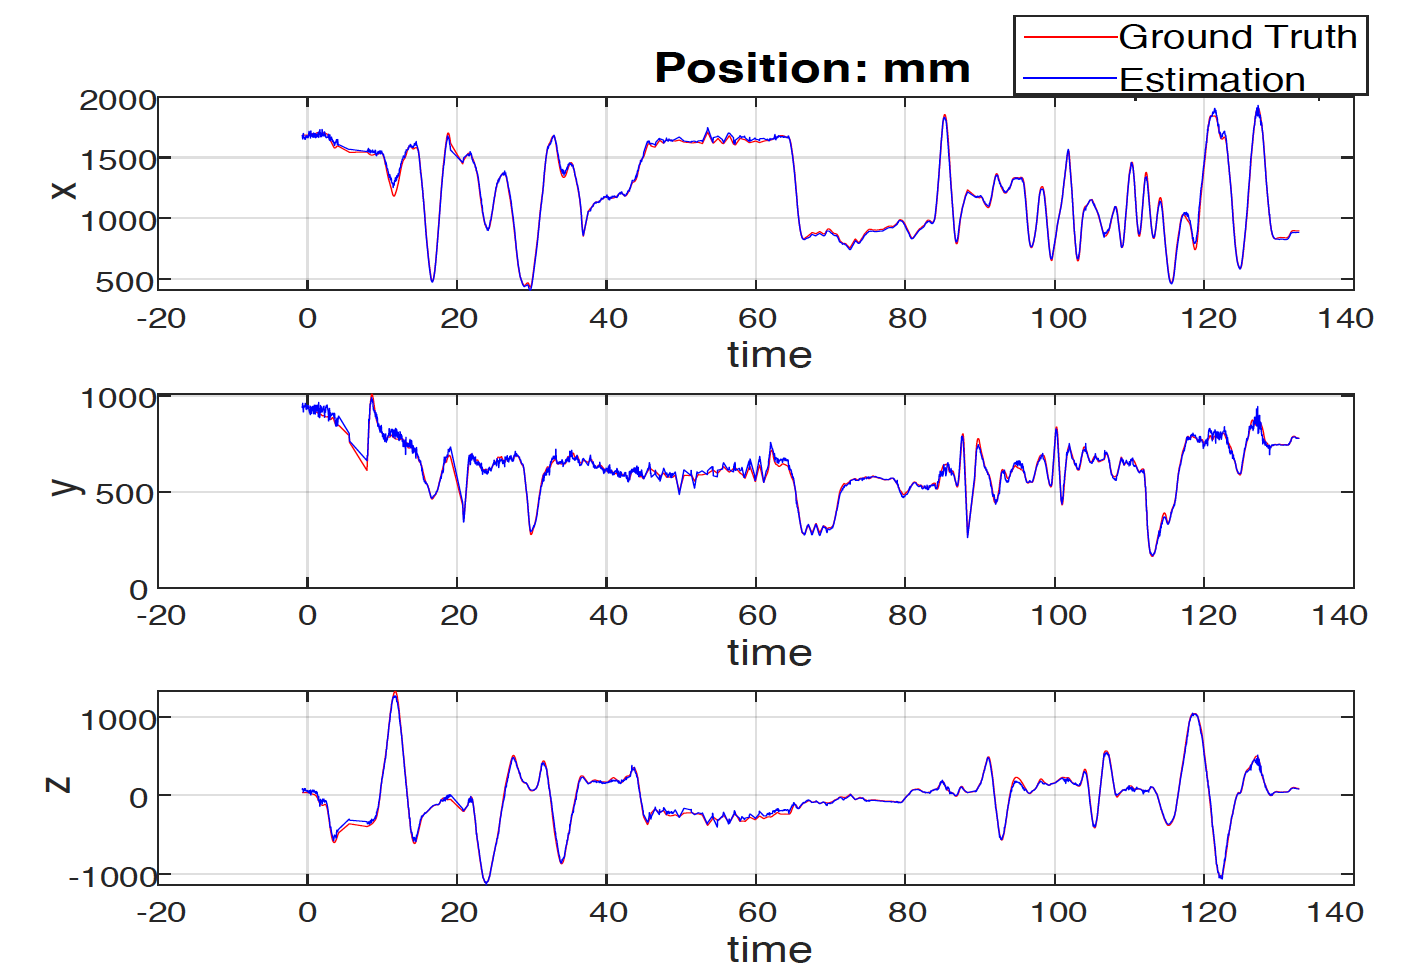
\includegraphics[width=0.5\textwidth]{figures/poster/poseest_t}
%		%	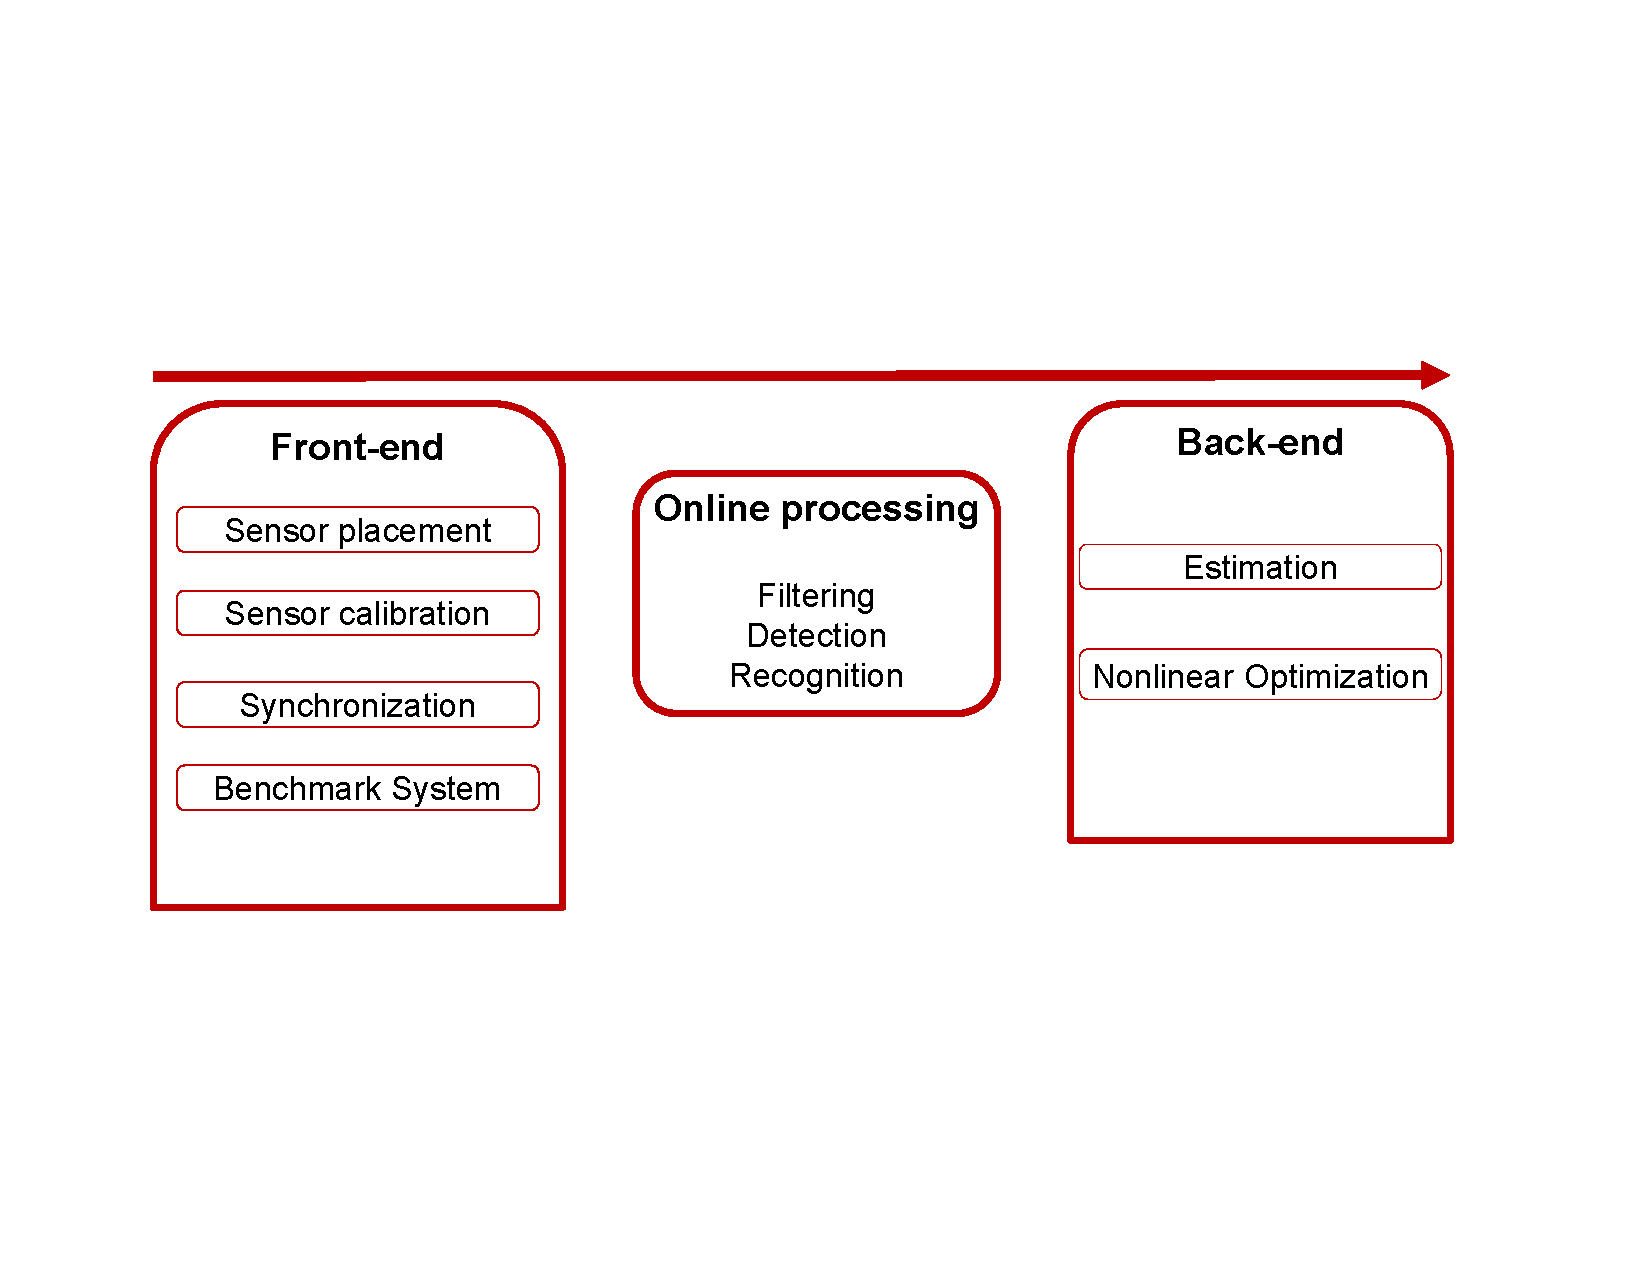
\includegraphics[width=0.3\textwidth]{figures/poster/system_bd}
%	}}
%	\framebox{\parbox{3.1in}{
%			\centering
%			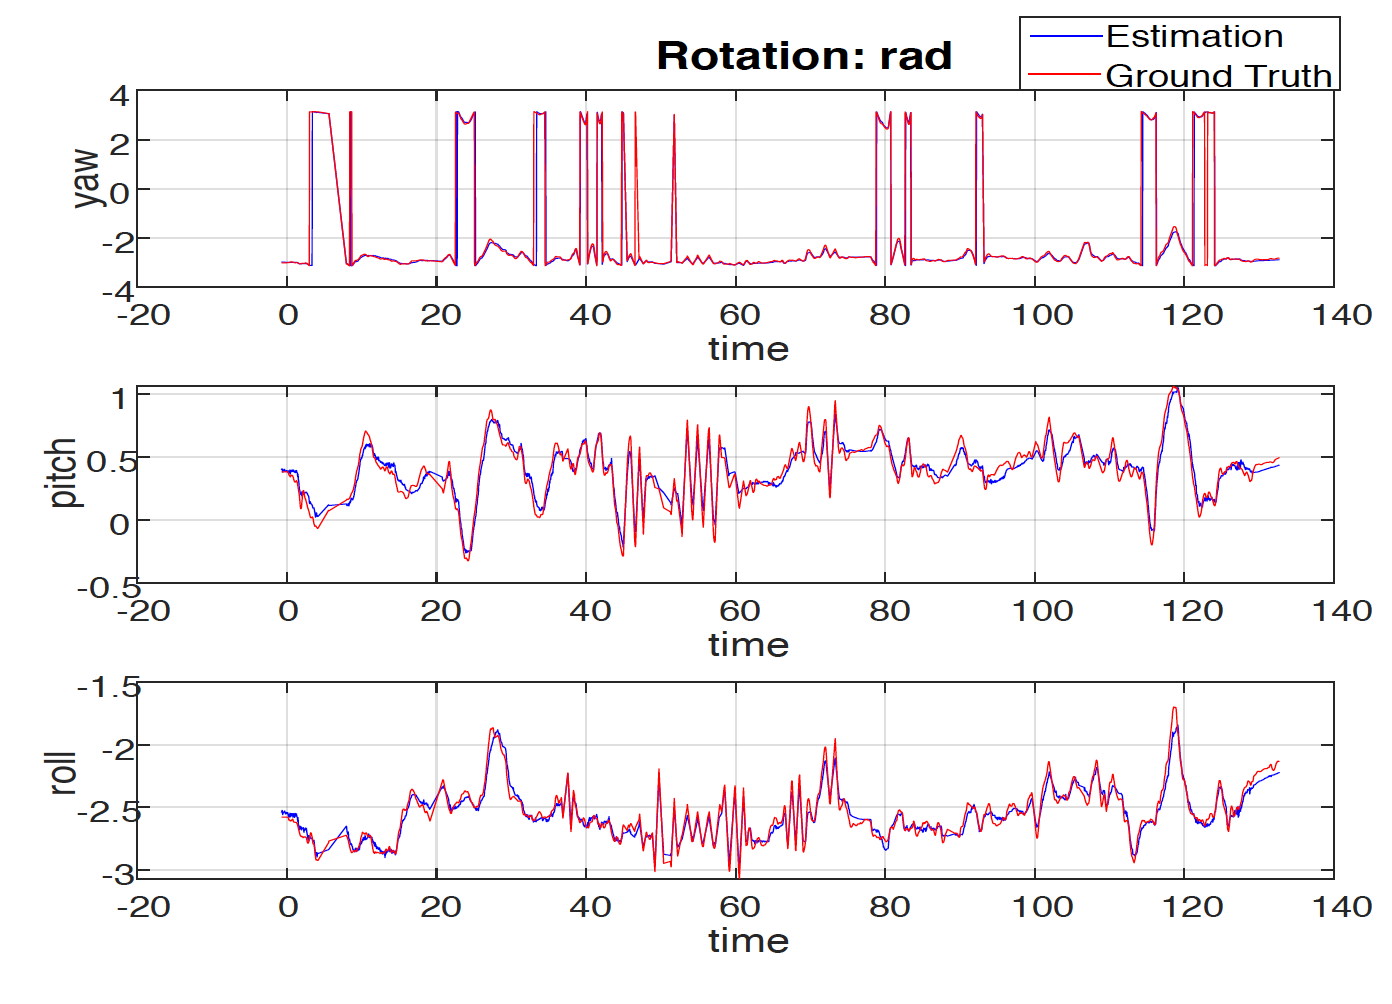
\includegraphics[width=0.5\textwidth]{figures/poster/poseest_r}
%			%	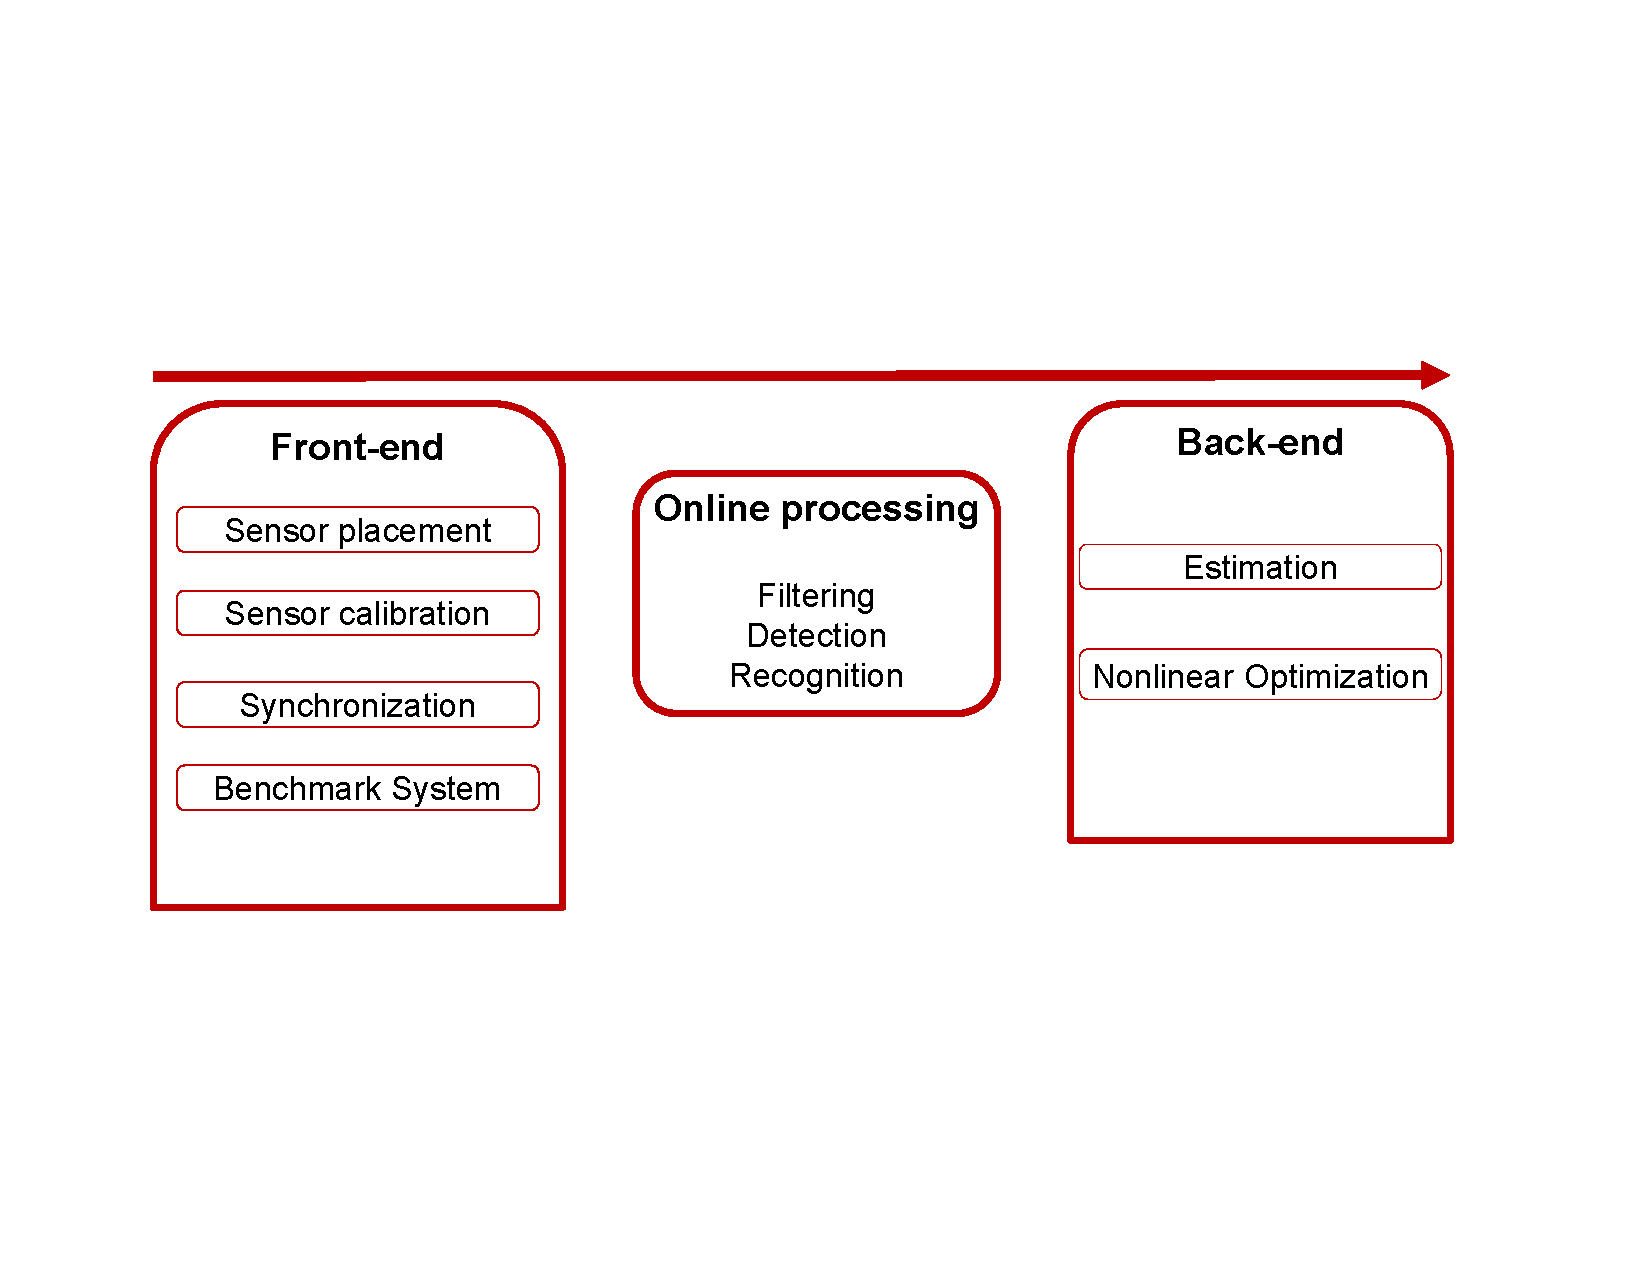
\includegraphics[width=0.3\textwidth]{figures/poster/system_bd}
%	}}
  }
  \vspace{-1cm}  
%%%%%%%%%%%%%%%%%%%%%%%%%%%%%%%%%%%%%%%%%%%%%%%%%%%%%%%%%%%%%%%%%%%%%%%%%%%%%%
% \headerbox{Lucas-Kanade Method}{name=lk,column=0,row=0,below=brc}{
%  Solve with least-square solution
%  \begin{align*}
%  \mathbf{u} = (\mathbf{A}^T\mathbf{A})^{-1}\mathbf{A}^T\mathbf{b},\ \mathbf{A}=[\mathbf{a}_1, \cdots, \mathbf{a}_k]^T
%  \end{align*}
%  }
%   \headerbox{Horn-Shunck Method}{name=hs,column=0,row=0,above=bottom}{
%	Add regularization on the smoothness of the flow and solve a joint minimization problem
%  \begin{align*}
%  E_{joint} = E+\int{\int}\alpha^2(||\bigtriangledown u||^2+||\bigtriangledown v||^2) dxdy
%  \end{align*}
%  The optimization problem is solved iteratively
%  \begin{align*}
%  u^{k+1}=\bar{u}^k-\frac{I_x(I_x\bar{u}^k+I_y\bar{v}^k+I_t)}{\alpha^2+I_x^2+I_y^2}\\
%  v^{k+1}=\bar{v}^k-\frac{I_y(I_x\bar{u}^k+I_y\bar{v}^k+I_t)}{\alpha^2+I_x^2+I_y^2}
%  \end{align*}
%  }
%%%%%%%%%%%%%%%%%%%%%%%%%%%%%%%%%%%%%%%%%%%%%%%%%%%%%%%%%%%%%%%%%%%%%%%%%%%%%%%
%\headerbox{Implementation}{name=lowrestracking,column=1,span=1,below=speed,below=contribution}{
%\paragraph{Conditioning} $\mathbf{Au=b}$ may be ill-posed. To deal with:
%\begin{itemize}
%\setlength\itemsep{0.1em}
%\item check the harmonic mean: $\frac{\text{det}(\mathbf{A})}{\text{tr}(\mathbf{A})} > \tau$.
%\item check the minimum eigenvalue: $\lambda_{min}> \tau$.
%\end{itemize}
%\paragraph{Gradient Kernel} To compute $I_x, I_y$, different kernels are applied:
%\begin{itemize}
%\setlength\itemsep{0.1em}
%\item $[-1,0,1]$.
%\item Derivative of Gaussian.
%\end{itemize}
%\paragraph{Weighting Kernel} To sum up the contributions from neighbouring pixels, the following kernels are applied:
%\begin{itemize}
%\setlength\itemsep{0.1em}
%\item Box filter.
%\item Gaussian Kernel.
%\end{itemize}
%\paragraph{Coarse-to-Fine} To deal with large movement, image pyramid is used to establish a coarse-to-fine flow estimation.
%\newline
%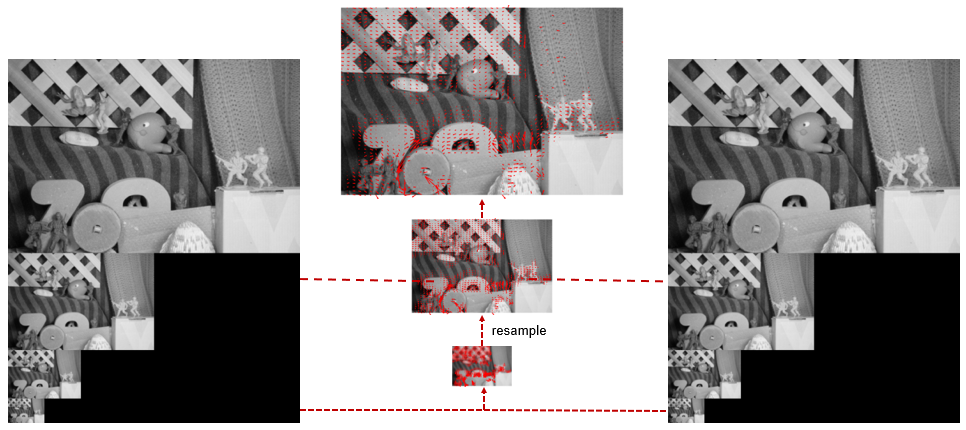
\includegraphics[width=1\linewidth]{figures/final.png}%
%\vspace{0.25em}
%\textbf{Coarse-to-Fine Optical Flow Estimation}.
%}
 %%%%%%%%%%%%%%%%%%%%%%%%%%%%%%%%%%%%%%%%%%%%%%%%%%%%%%%%%%%%%%%%%%%%%%%%%%%%%%
   \headerbox{Navigation}{name=speed,column=2,row=0,span=2}{
 %%%%%%%%%%%%%%%%%%%%%%%%%%%%%%%%%%%%%%%%%%%%%%%%%%%%%%%%%%%%%%%%%%%%%%%%%%%%%%
% \framebox{\parbox{3.1in}{
% Solve QP and SDP alternatively: 
% \begin{itemize}
% 	\item No requirement for a pre-determined time allocation or initial guess of total time spending.
% 	\item Propose to model collision avoidance in an affine function by leveraging two supporting planes.
% \end{itemize}
%	}}
	\setlength{\fboxrule}{0.0pt}
  \framebox{\parbox{6.3in}{
\begin{tabular}{c@{\hspace{0.05em}}c@{\hspace{0.2em}}c@{\hspace{0.1em}}c@{\hspace{0.2em}}c@{\hspace{0.1em}}c@{\hspace{0.1em}}c}
	\centering
	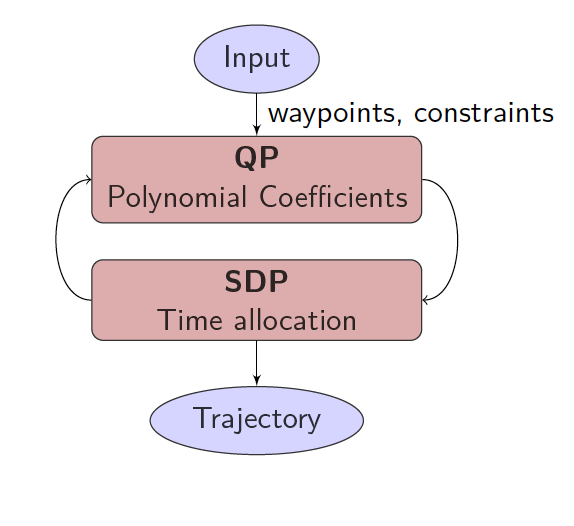
\includegraphics[width=0.23\linewidth]{figures/poster/nav}&
	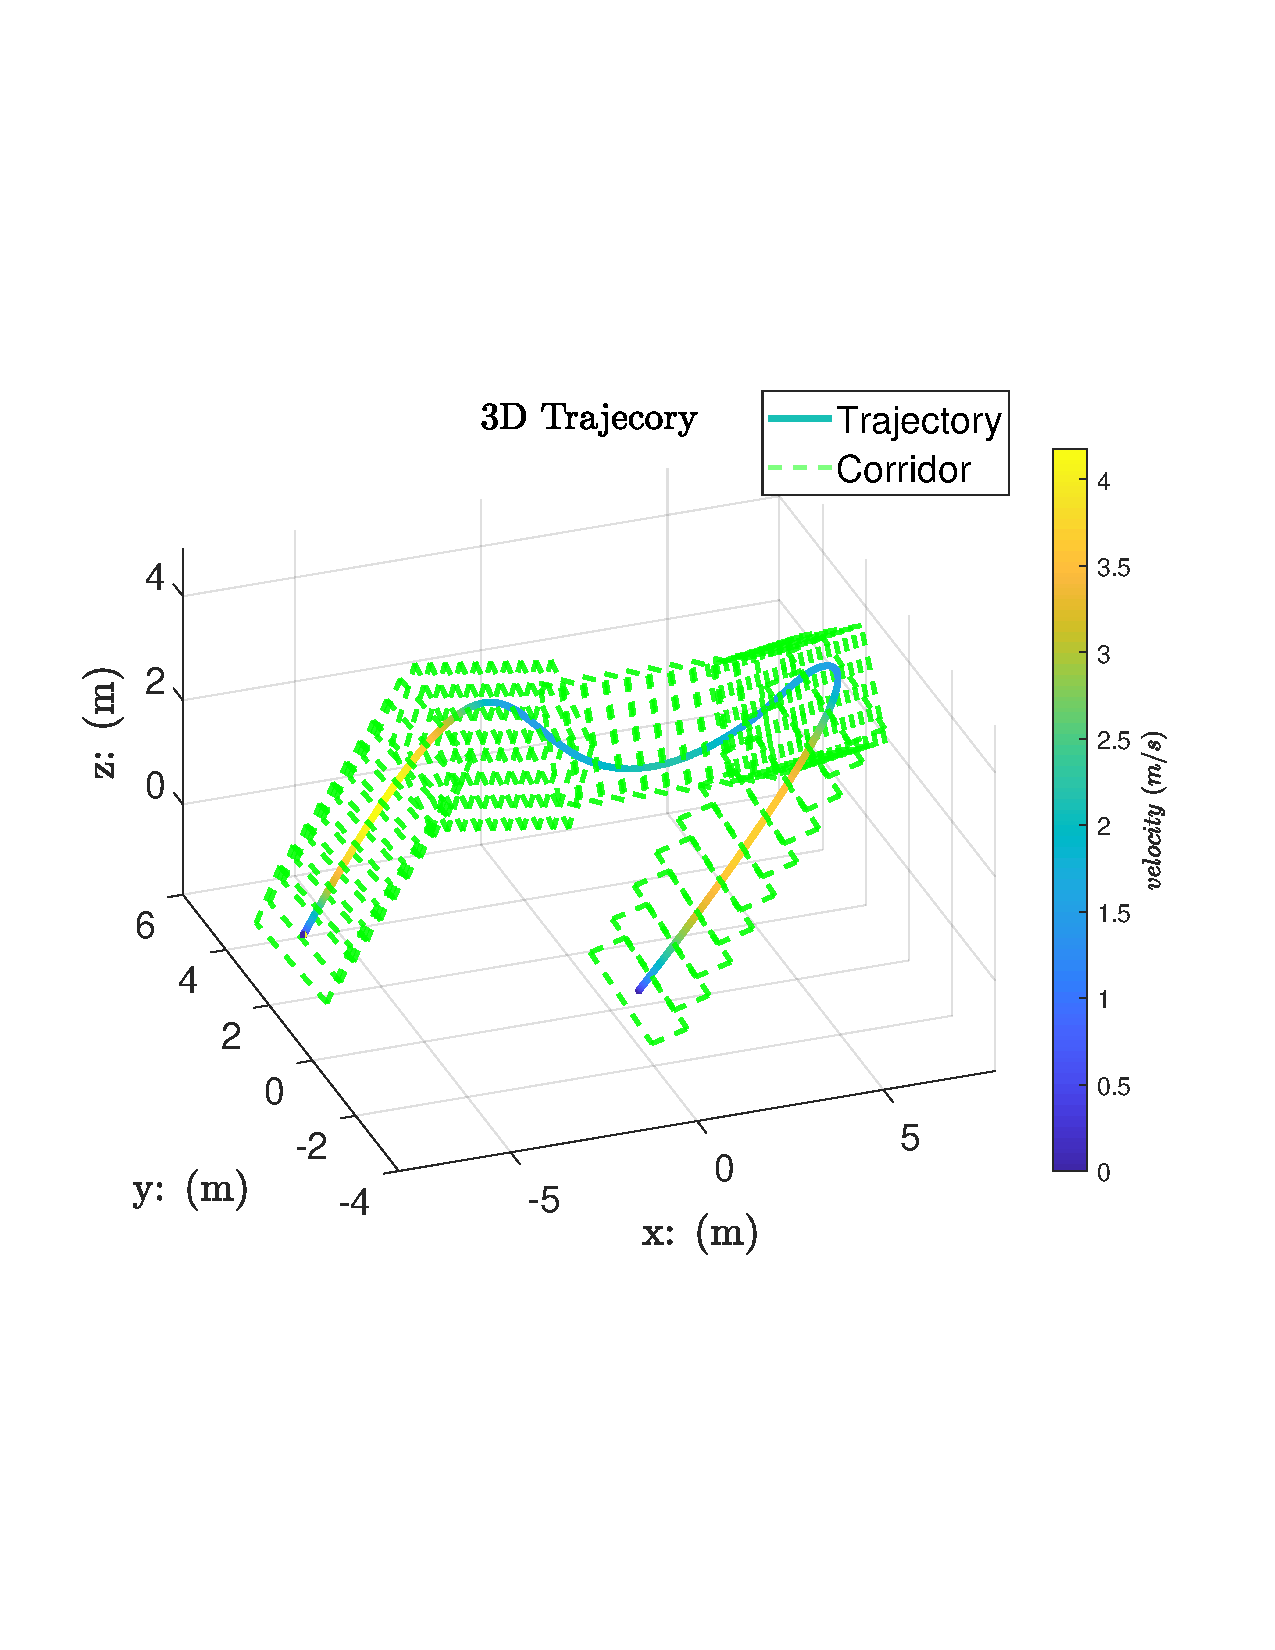
\includegraphics[width=0.23\linewidth]{figures/poster/corridor_trajss}&
	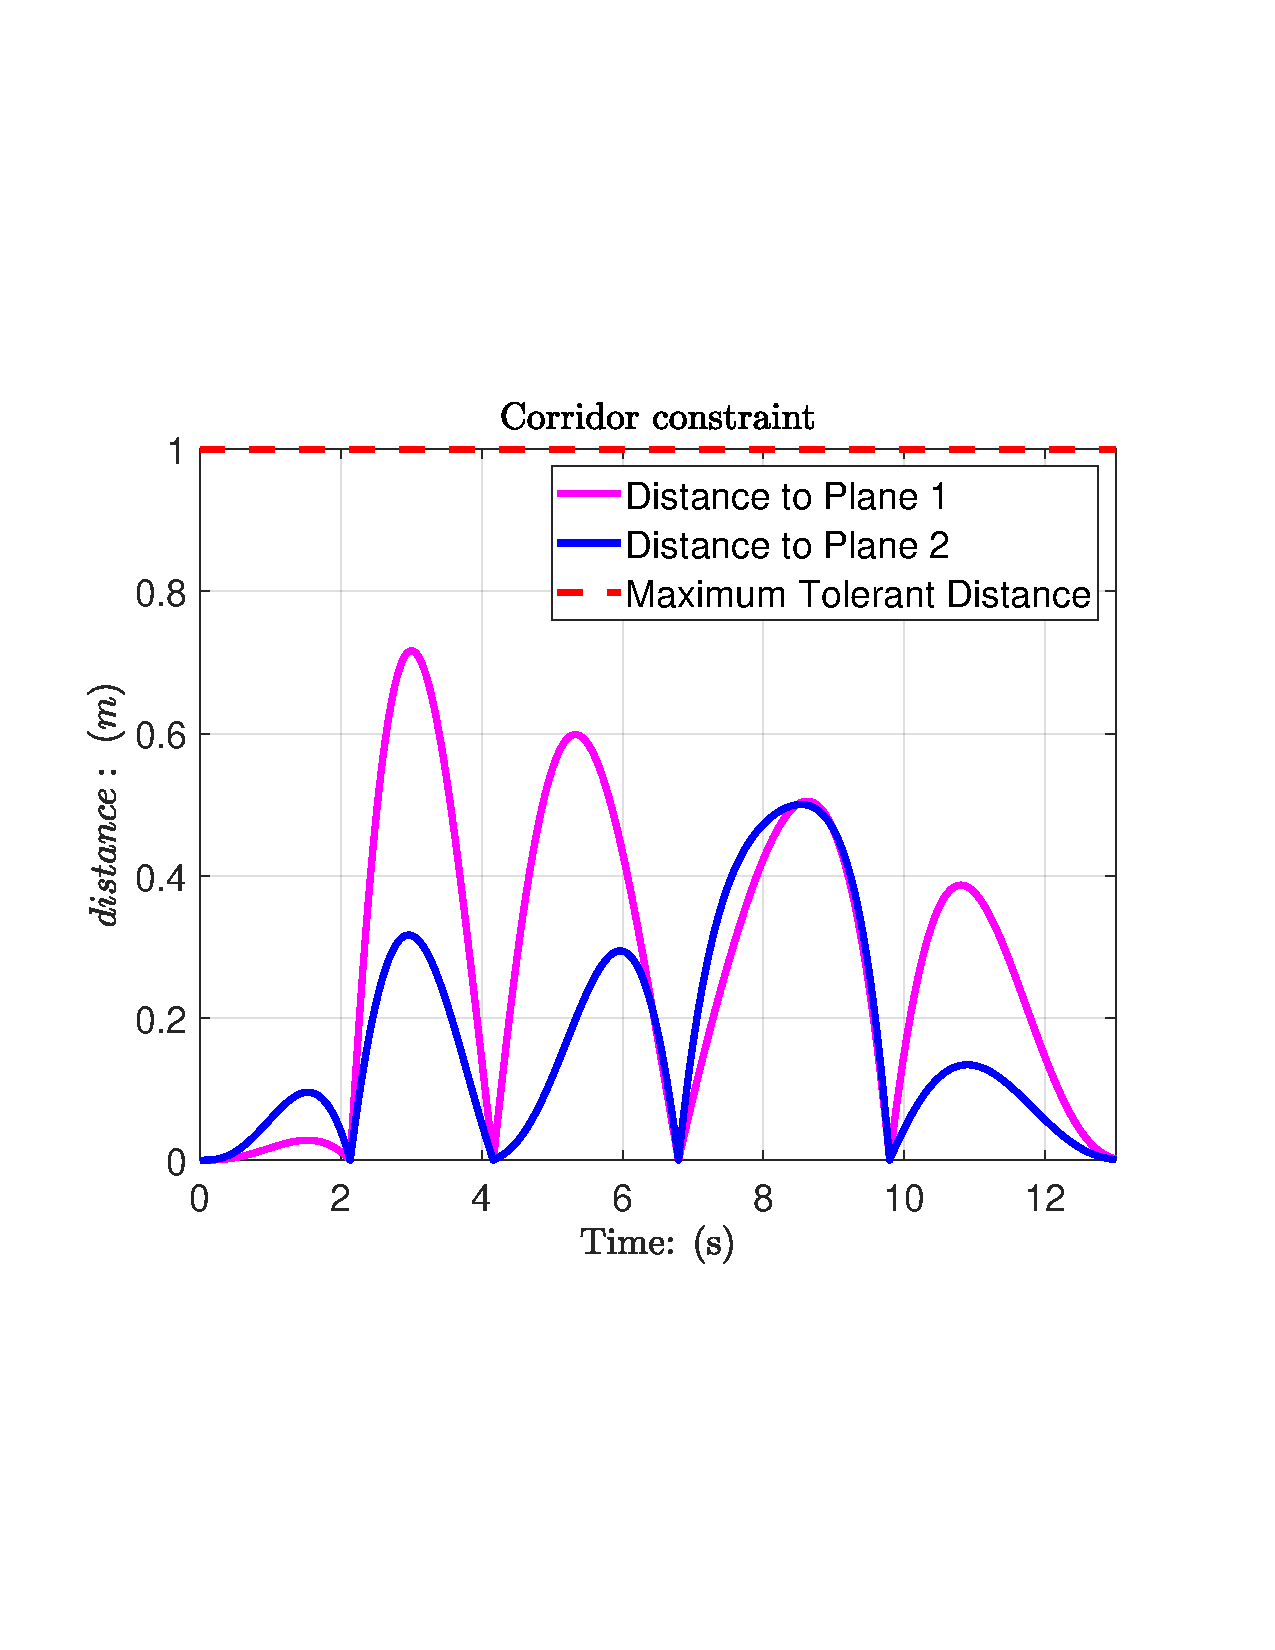
\includegraphics[width=0.23\linewidth]{figures/poster/corridor_distance}&
	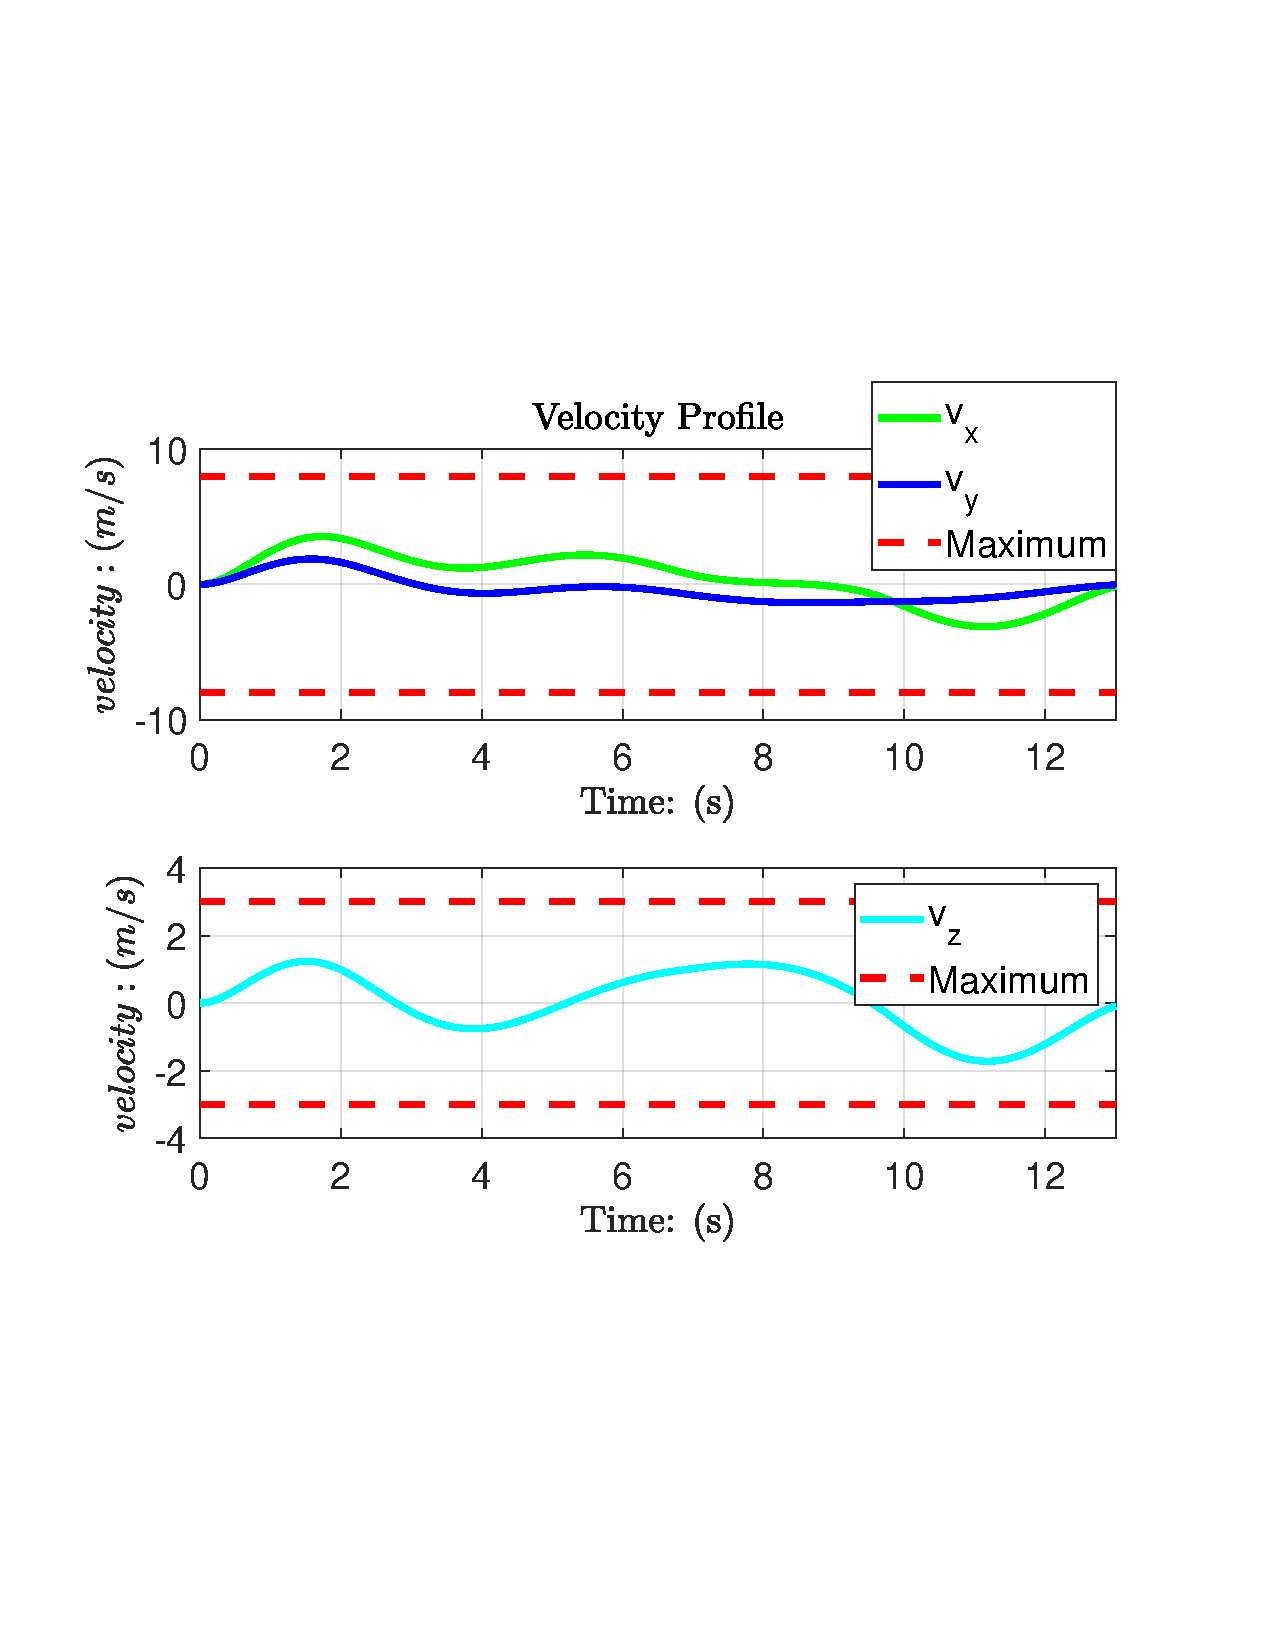
\includegraphics[width=0.23\linewidth]{figures/poster/corridor_velpro} \\[-0.1em]
	\smaller \textbf{Schematic Diagram} & \smaller \textbf{Trajectory} &  \smaller \textbf{Distance to Cooridor} & \smaller \textbf{Vel Profile}\\[-0.1em]
	\centering
	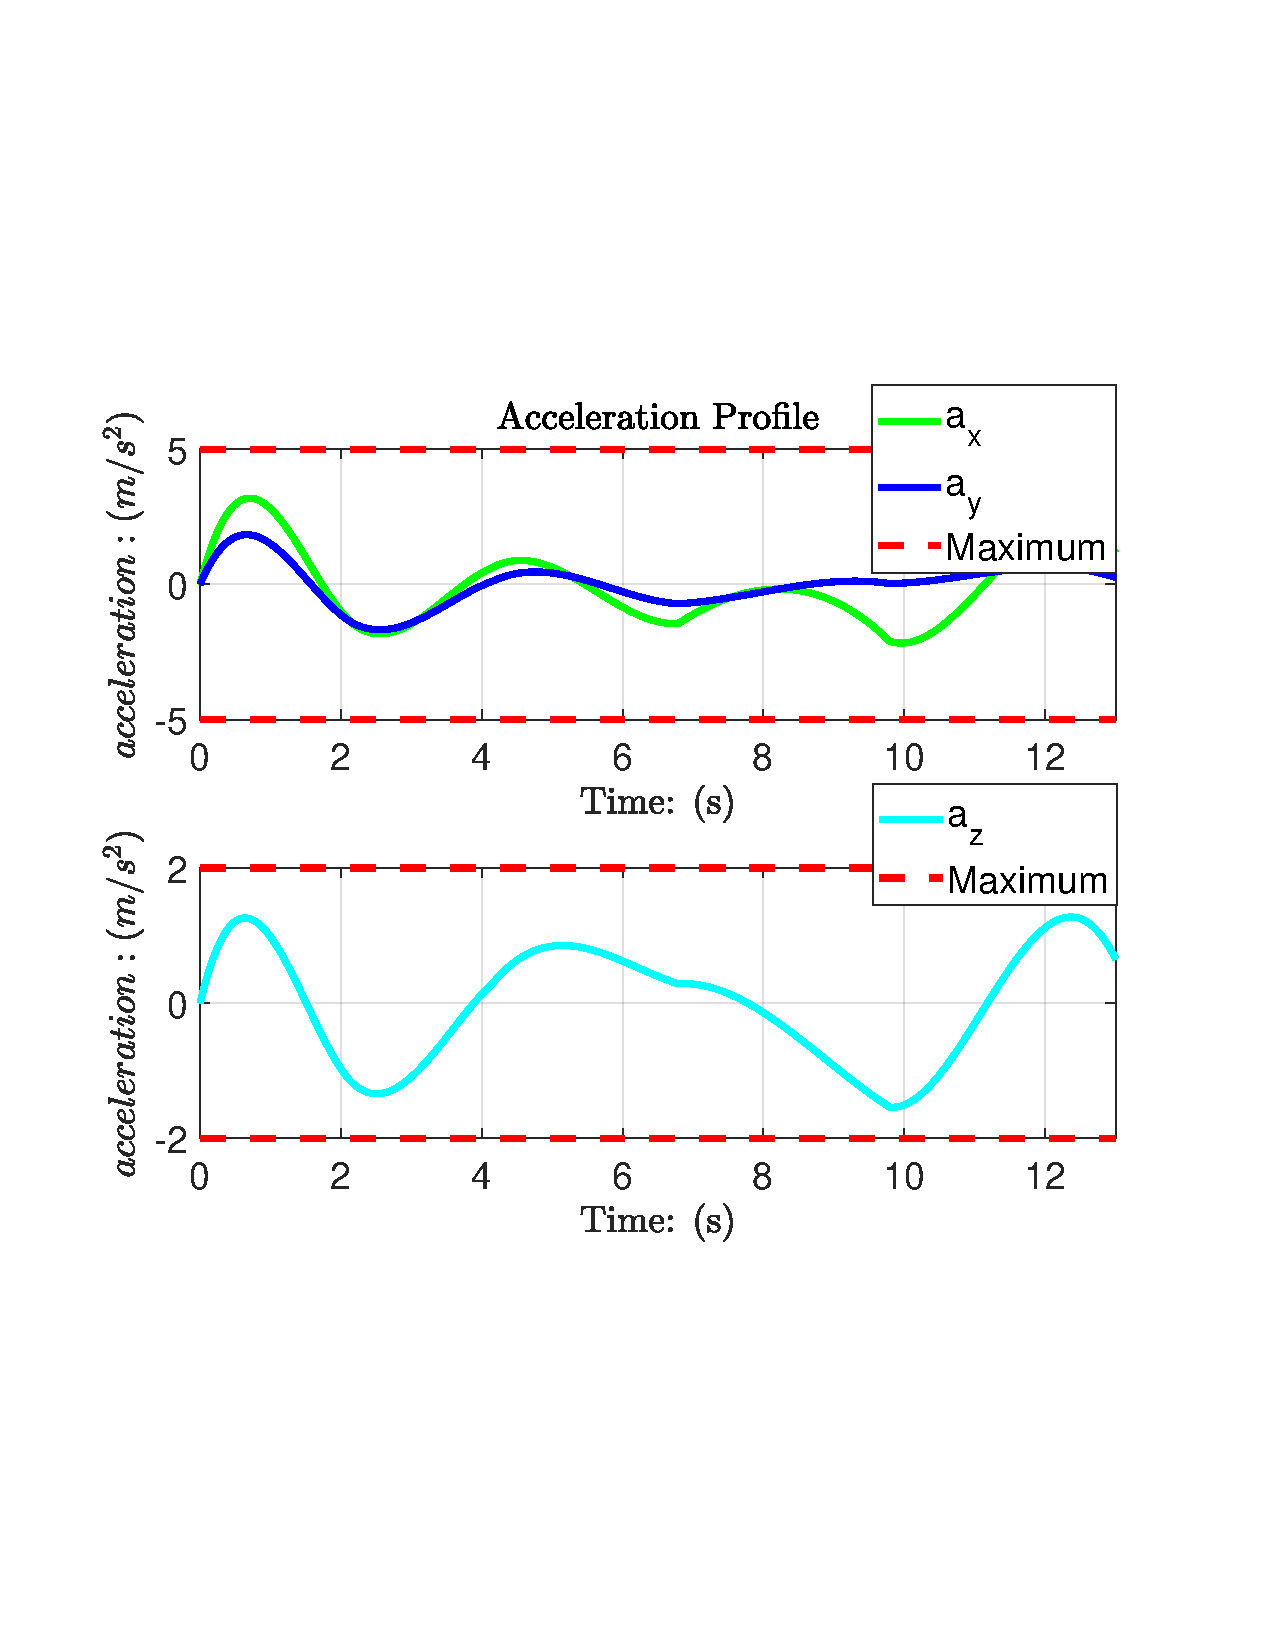
\includegraphics[width=0.23\linewidth]{figures/poster/corridor_accpro}&
	\includegraphics[width=0.23\linewidth]{figures/poster/Perlins.png}&
	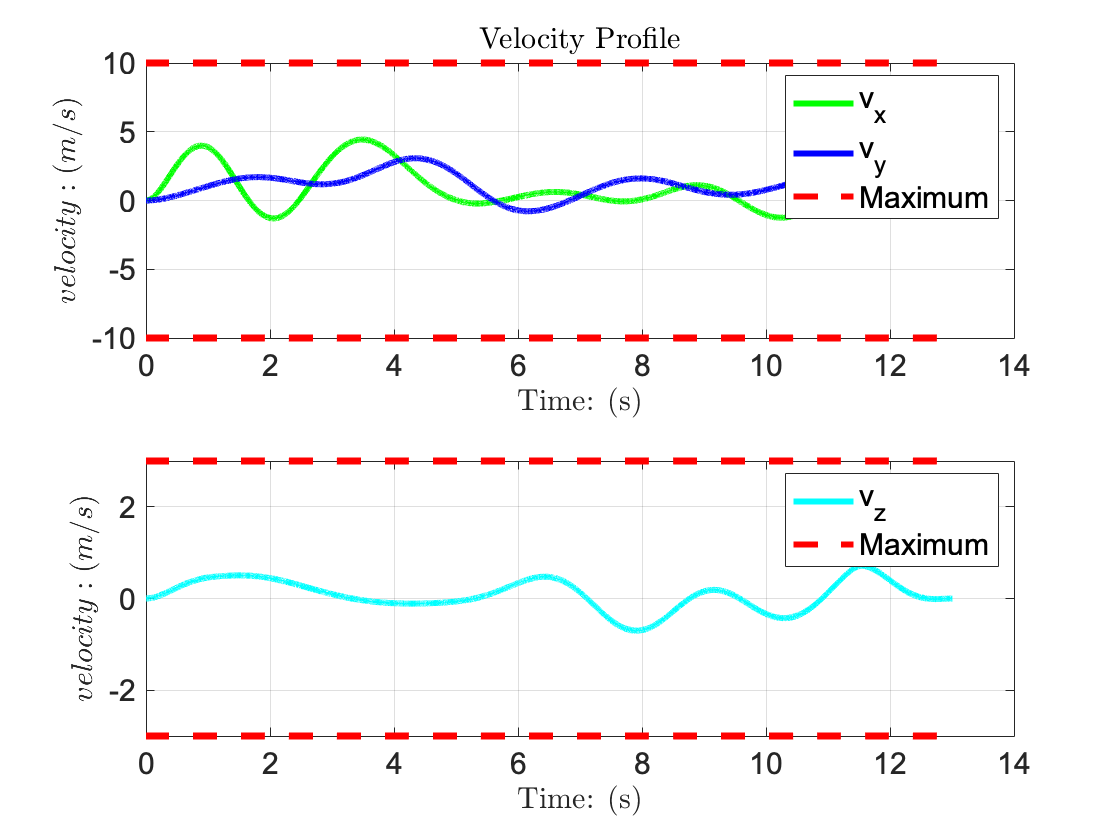
\includegraphics[width=0.23\linewidth]{figures/poster/perlin_vel_pro} &
	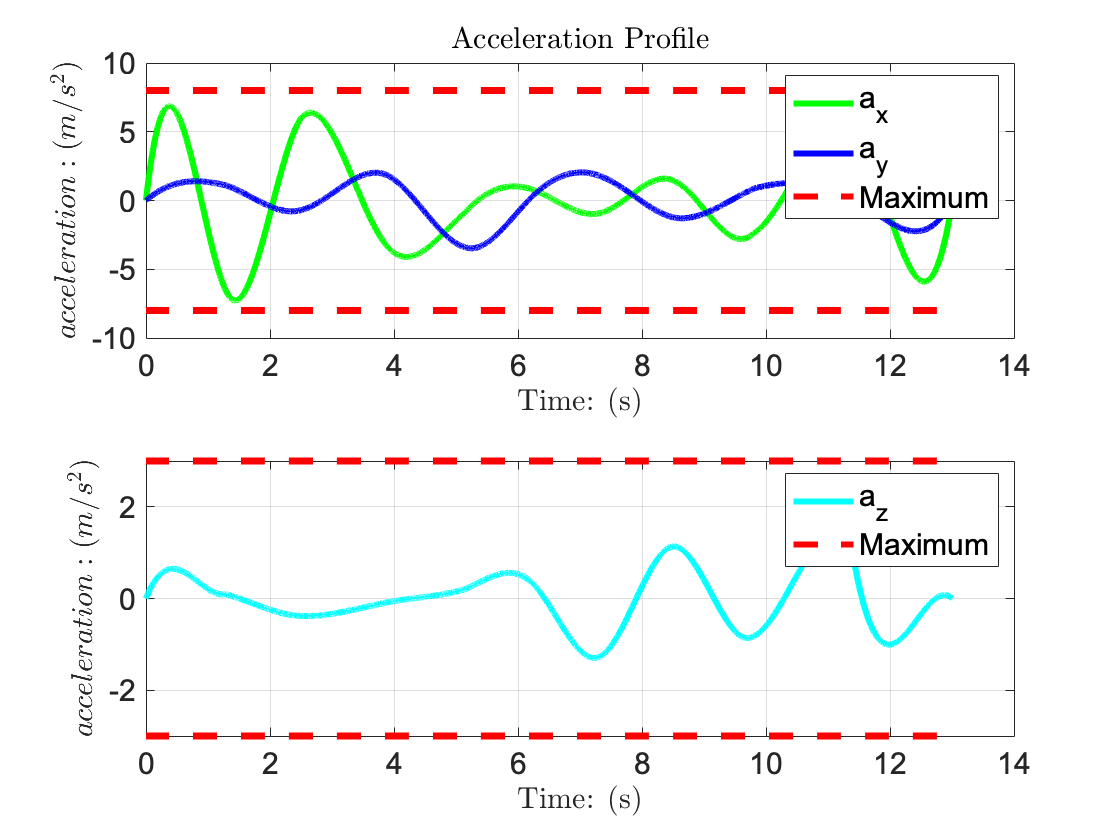
\includegraphics[width=0.23\linewidth]{figures/poster/perlin_acc_pro}
	\\[-0.1em]
	\smaller \textbf{Acc Profile} & \smaller \textbf{Perlin Noise Map} & \smaller \textbf{Vel Profile} & \smaller \textbf{Acc Profile}
\end{tabular}  	  	
  }}
   }
%
 %%%%%%%%%%%%%%%%%%%%%%%%%%%%%%%%%%%%%%%%%%%%%%%%%%%%%%%%%%%%%%%%%%%%%%%%%%%%%%
   \headerbox{References}{name=references,column=0,span=2,above=bottom}{
 %%%%%%%%%%%%%%%%%%%%%%%%%%%%%%%%%%%%%%%%%%%%%%%%%%%%%%%%%%%%%%%%%%%%%%%%%%%%%%
%     
     \bibliographystyle{ieee}
     \renewcommand{\section}[2]{\vskip 0.05em}
       \begin{thebibliography}{99}\itemsep=-0.01em
		\setlength{\baselineskip}{0.4em}
		\smaller
\bibitem{flow:lucas} \smaller Hu, X., et al. A Novel Robust Approach for
Correspondence-Free Extrinsic Calibration. 2019 IEEE/RSJ International Conference
on Intelligent Robots and Systems (IROS 2019).
\bibitem{flow:horns}  Hu, X., Olesen, D., \& Knudsen, P. (2019). Trajectory Generation Using Semidefinite Programming For Multi-Rotors. In Proceedings of the European Control Conference (ECC 2019) (pp. 2577-2582 ). IEEE.
\bibitem{flow:ln}  Hu, X., Jakobsen, J., Knudsen, P., \& Wei , J. (2018). Accurate Fiducial Mapping For Pose Estimation Using Manifold Optimization. In 2018 International Conference on Indoor Positioning and Indoor Navigation (IPIN) (pp. 206-212). 
       \end{thebibliography}
   }
 %%%%%%%%%%%%%%%%%%%%%%%%%%%%%%%%%%%%%%%%%%%%%%%%%%%%%%
   \headerbox{Calibration\&Synchronization}{name=tracking,column=2,span=2,below=speed,above=bottom}{
   %%%%%%%%%%%%%%%%%%%%%%%%%%%%%%%%%%%%%%%%%%%%%%%%%%%%%
     	\setlength{\fboxrule}{0.0pt}
     \framebox{\parbox{6.3in}{
     		\centering
     		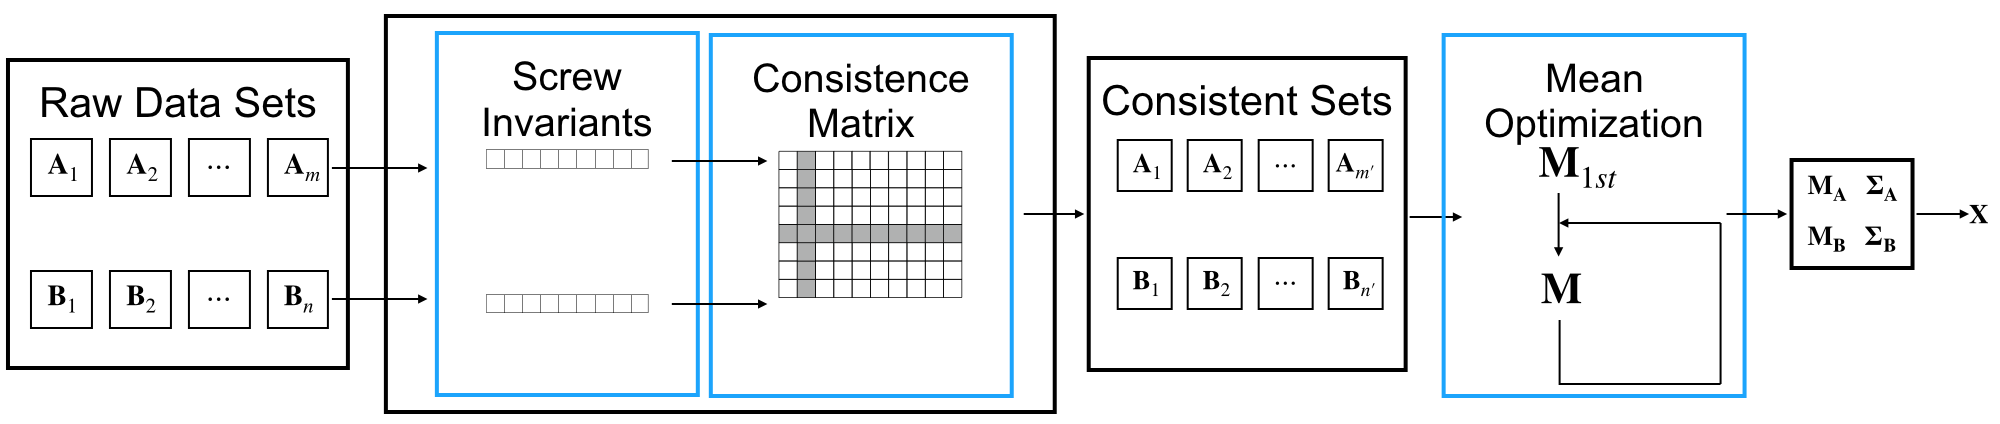
\includegraphics[width=0.8\textwidth]{figures/poster/13.png}
 	}}
 \begin{tabular}{c@{\hspace{0.05em}}c@{\hspace{0.2em}}c@{\hspace{0.1em}}c@{\hspace{0.2em}}c@{\hspace{0.1em}}c@{\hspace{0.1em}}c}
 	\centering
 	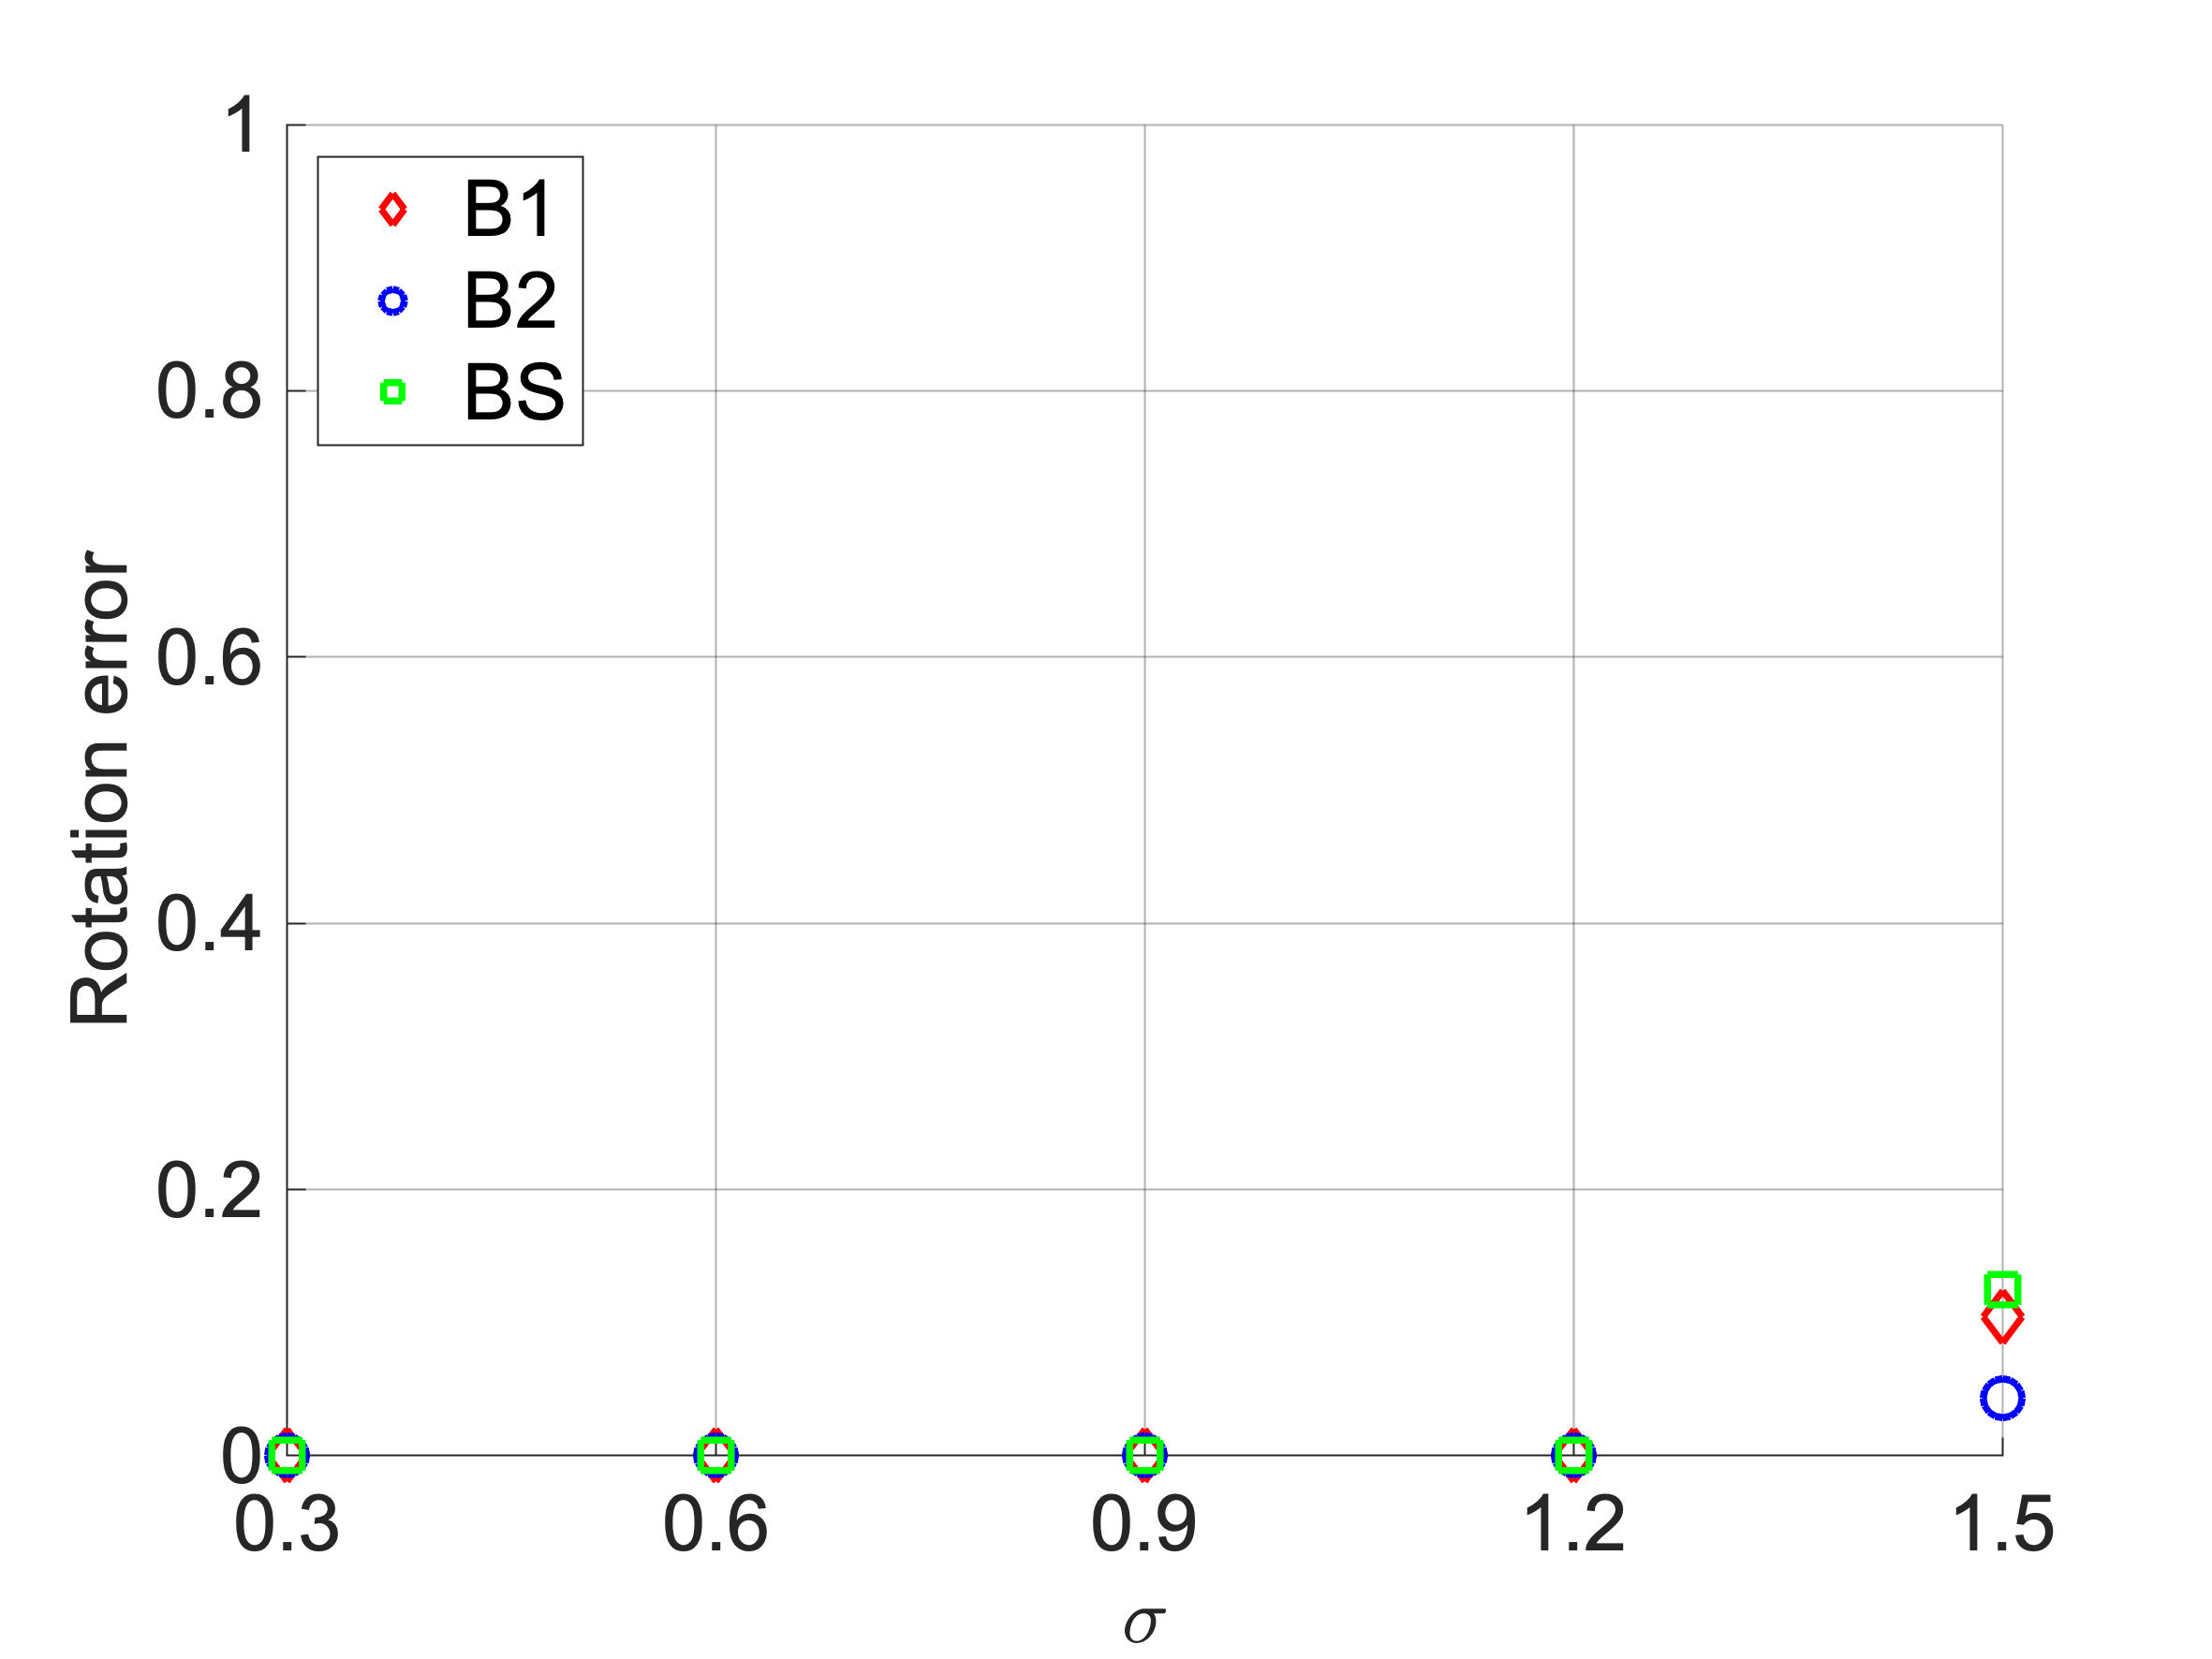
\includegraphics[width=0.22\linewidth]{figures/poster/res_1_r.png}&
 	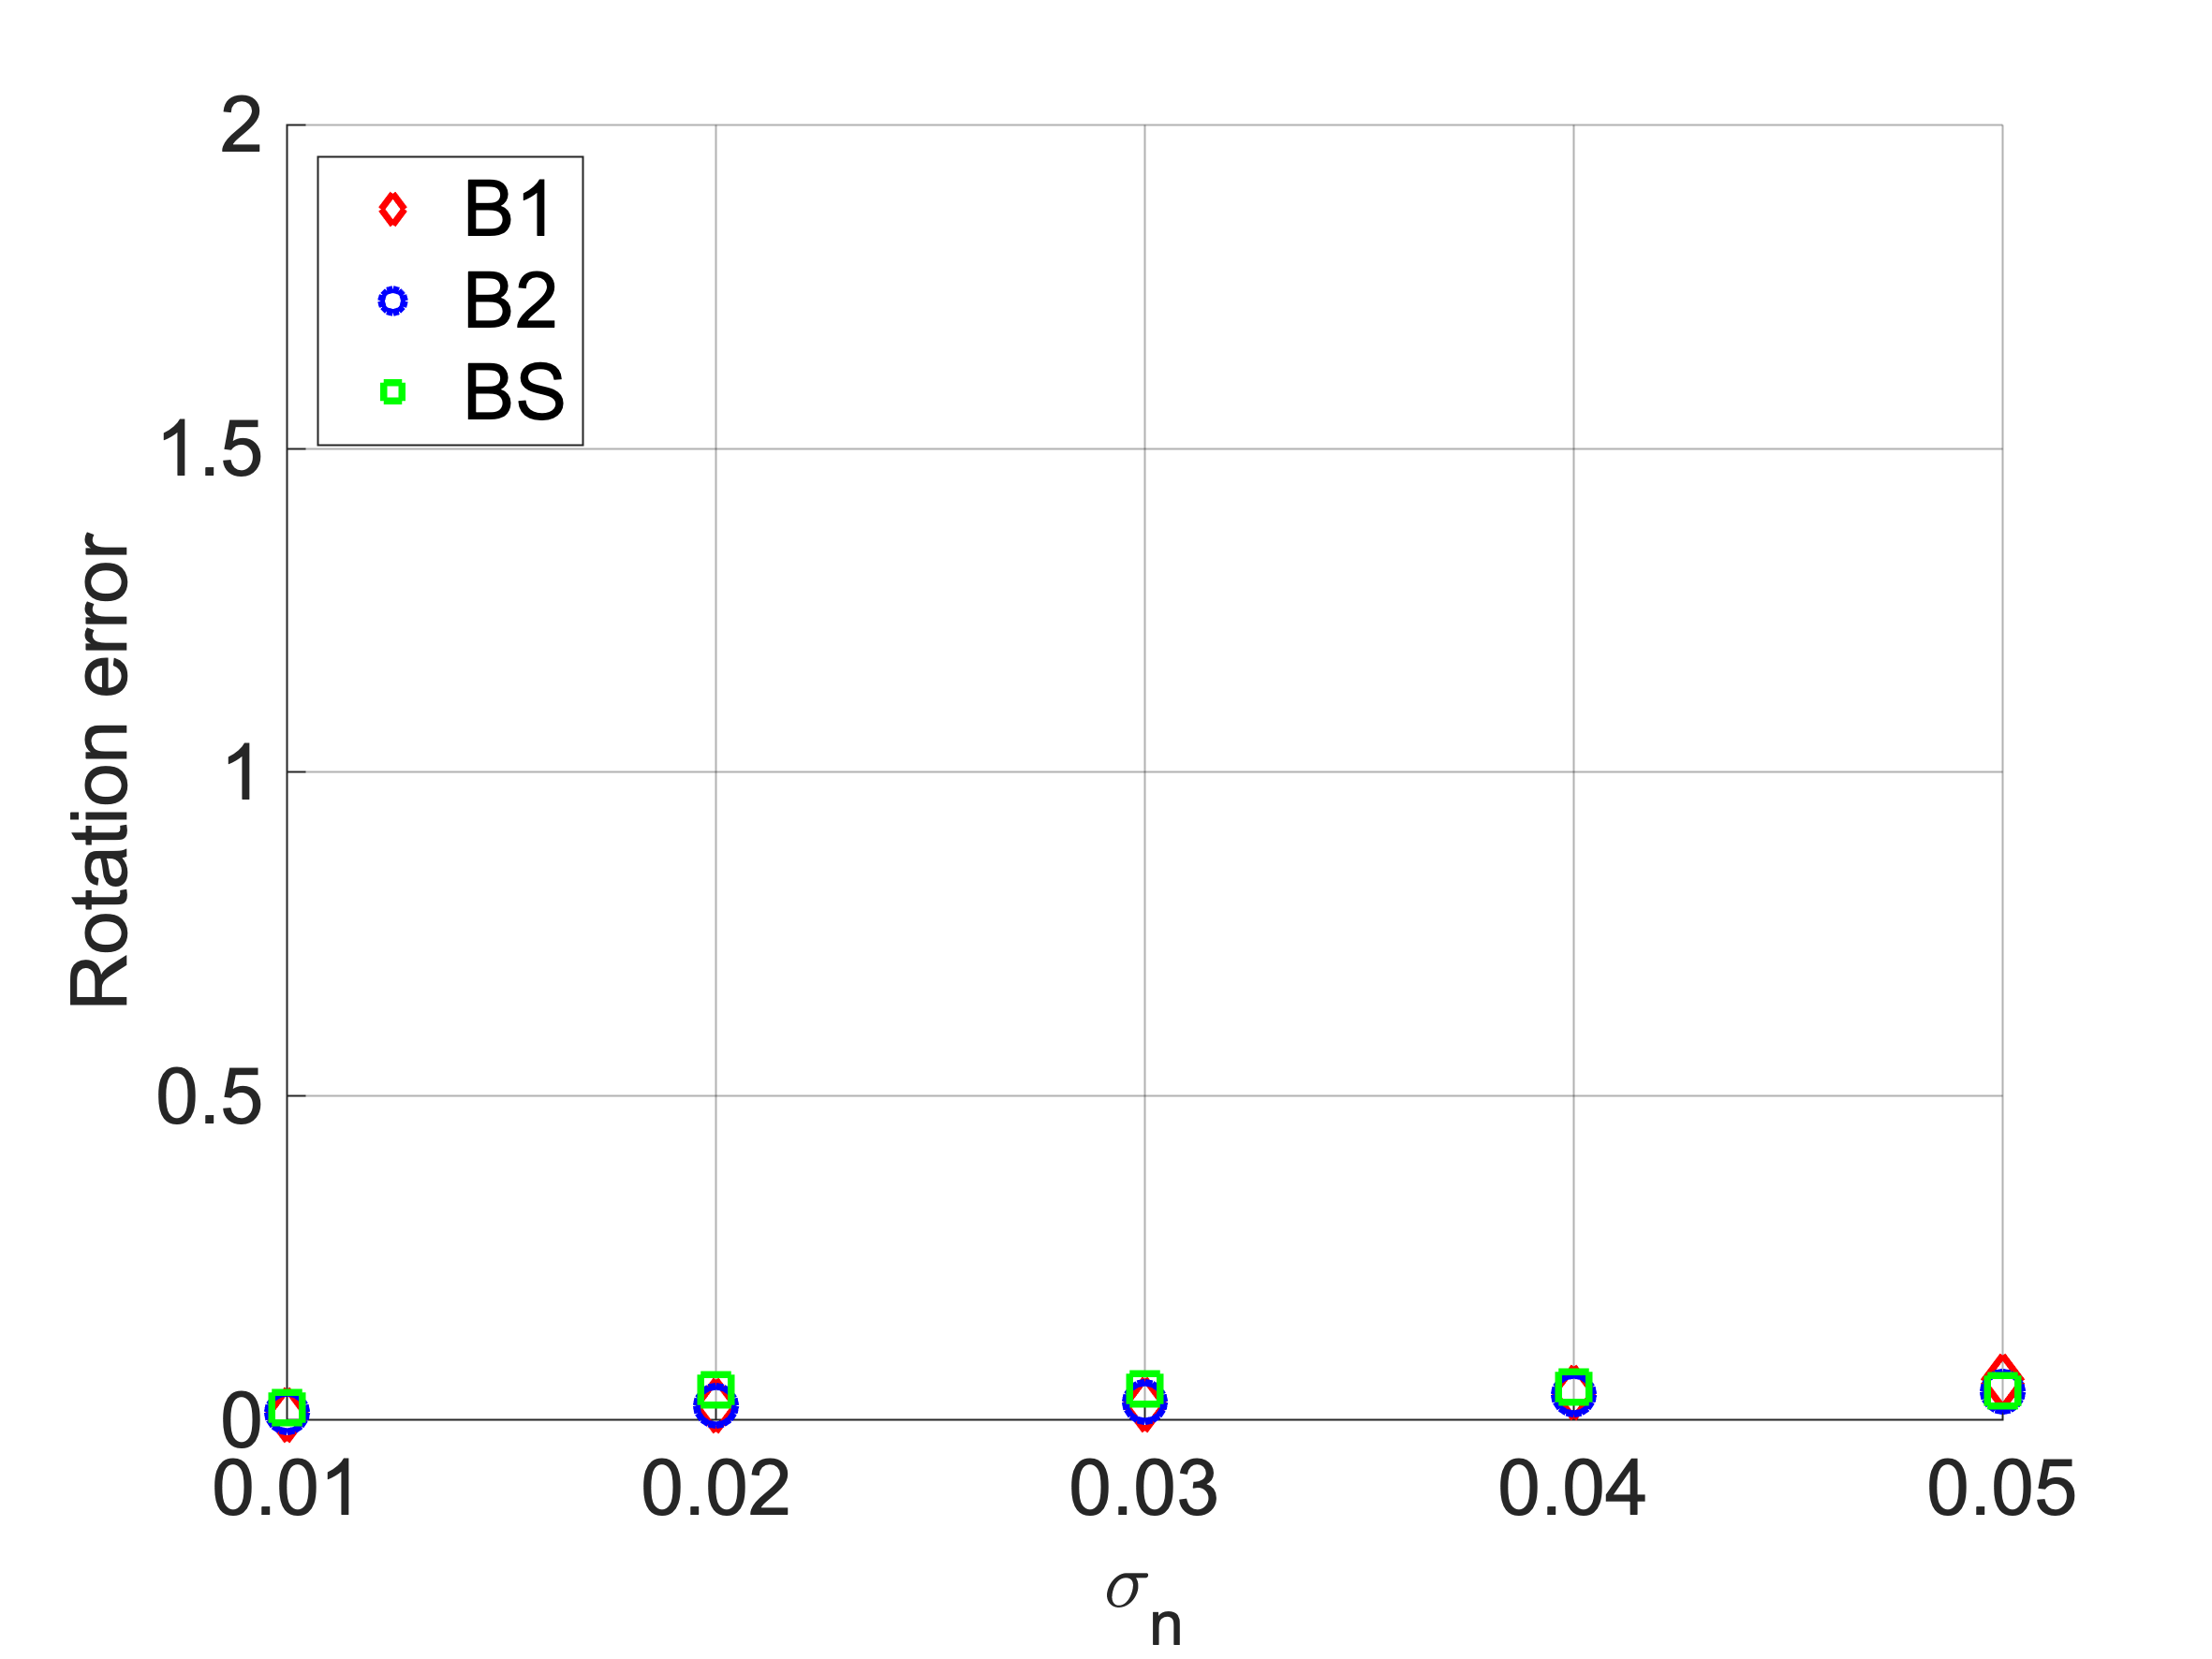
\includegraphics[width=0.22\linewidth]{figures/poster/res_3_r.png}&
 	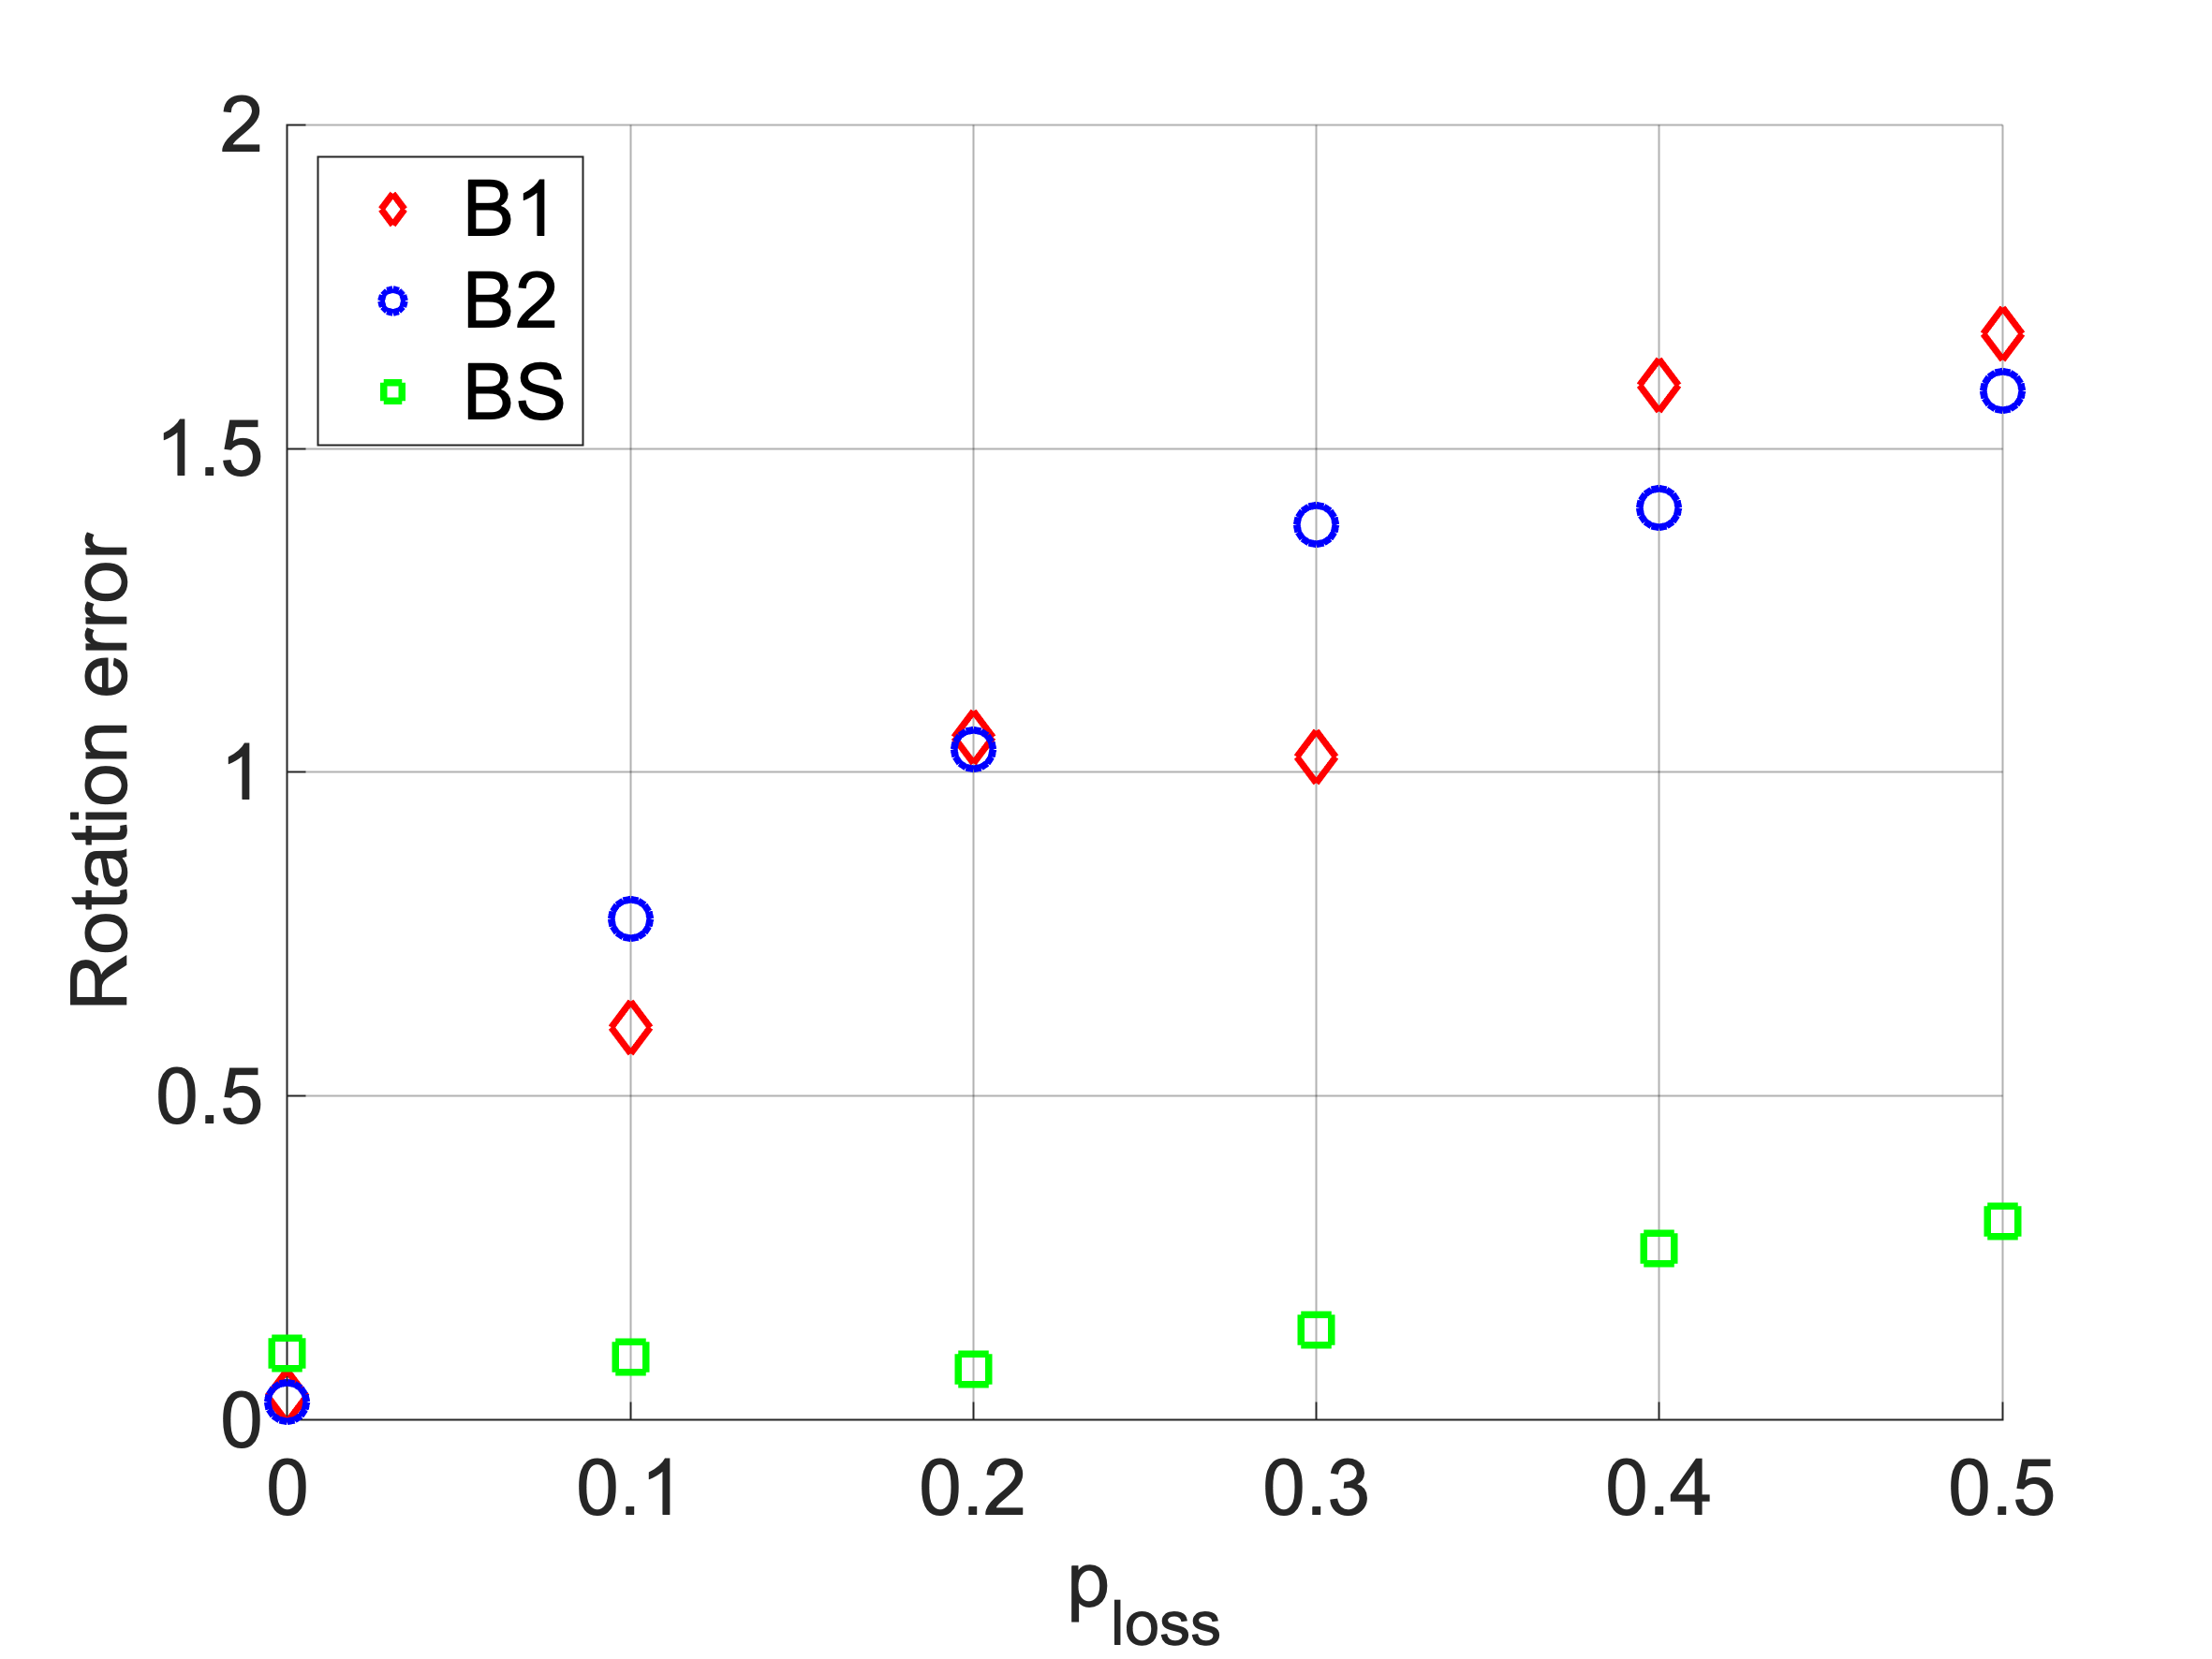
\includegraphics[width=0.22\linewidth]{figures/poster/res_4_r.png}&
 	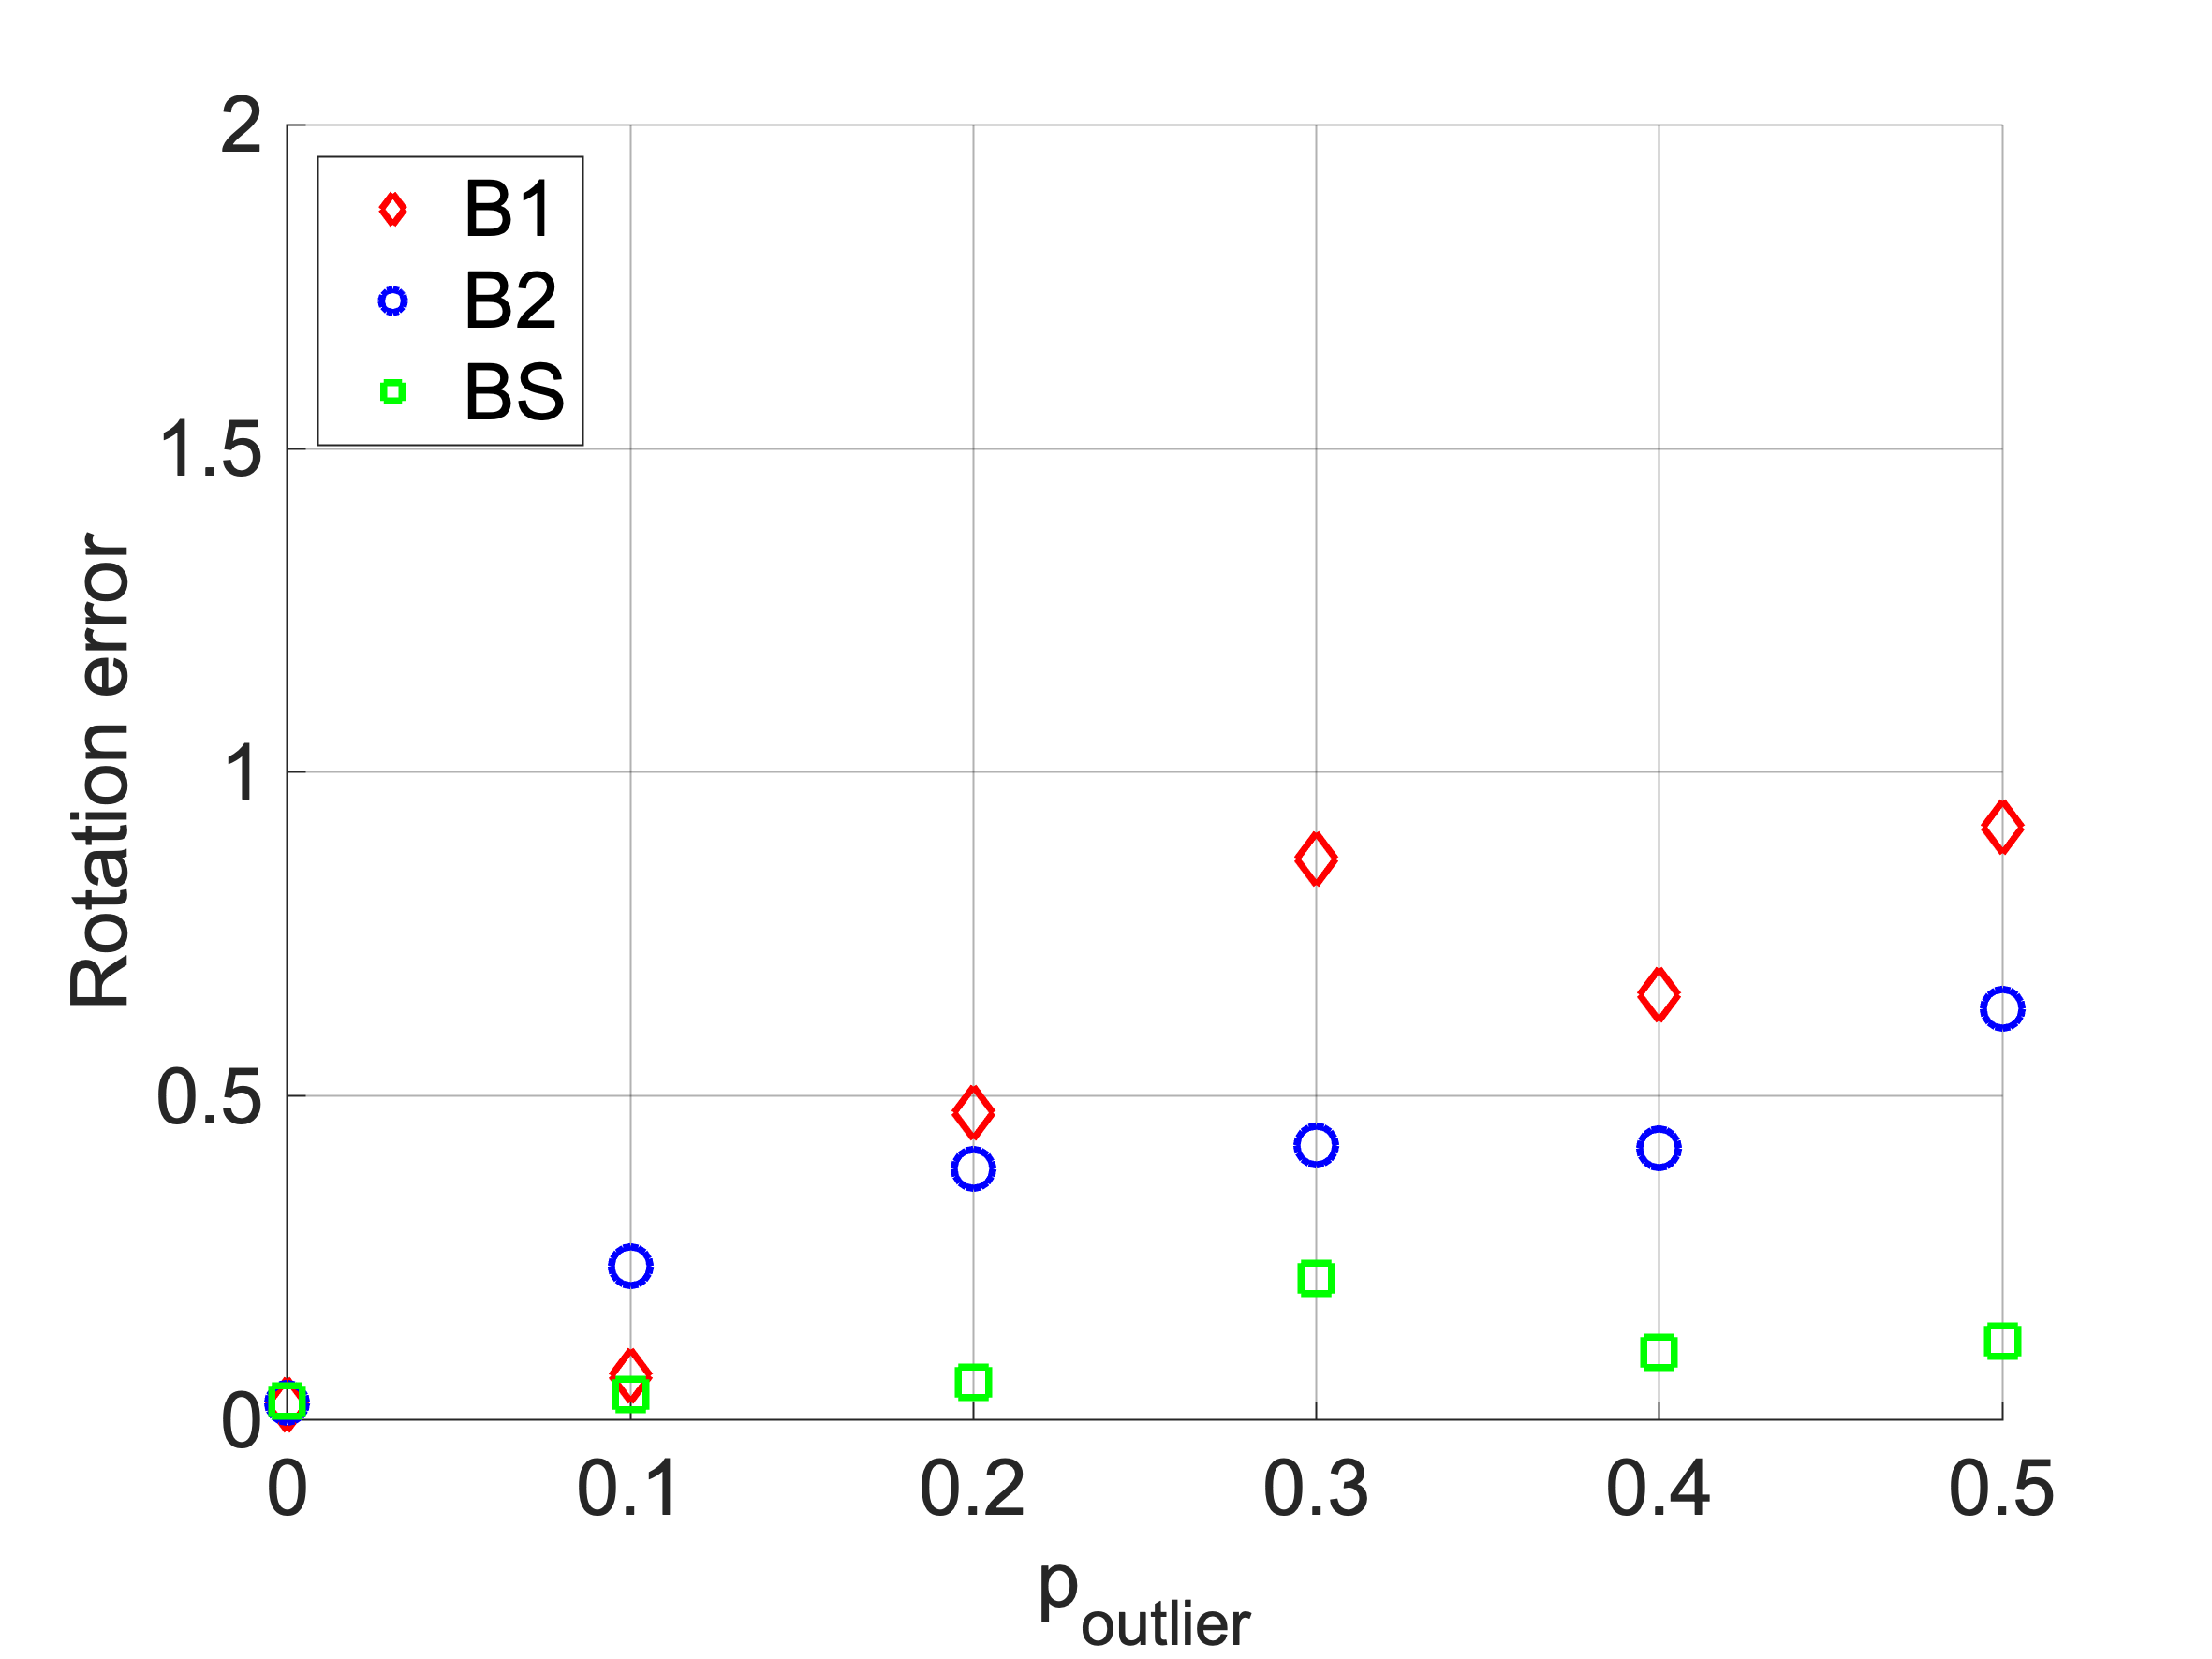
\includegraphics[width=0.22\linewidth]{figures/poster/res_5_r.png}\\[-0.1em]
 	\centering
 	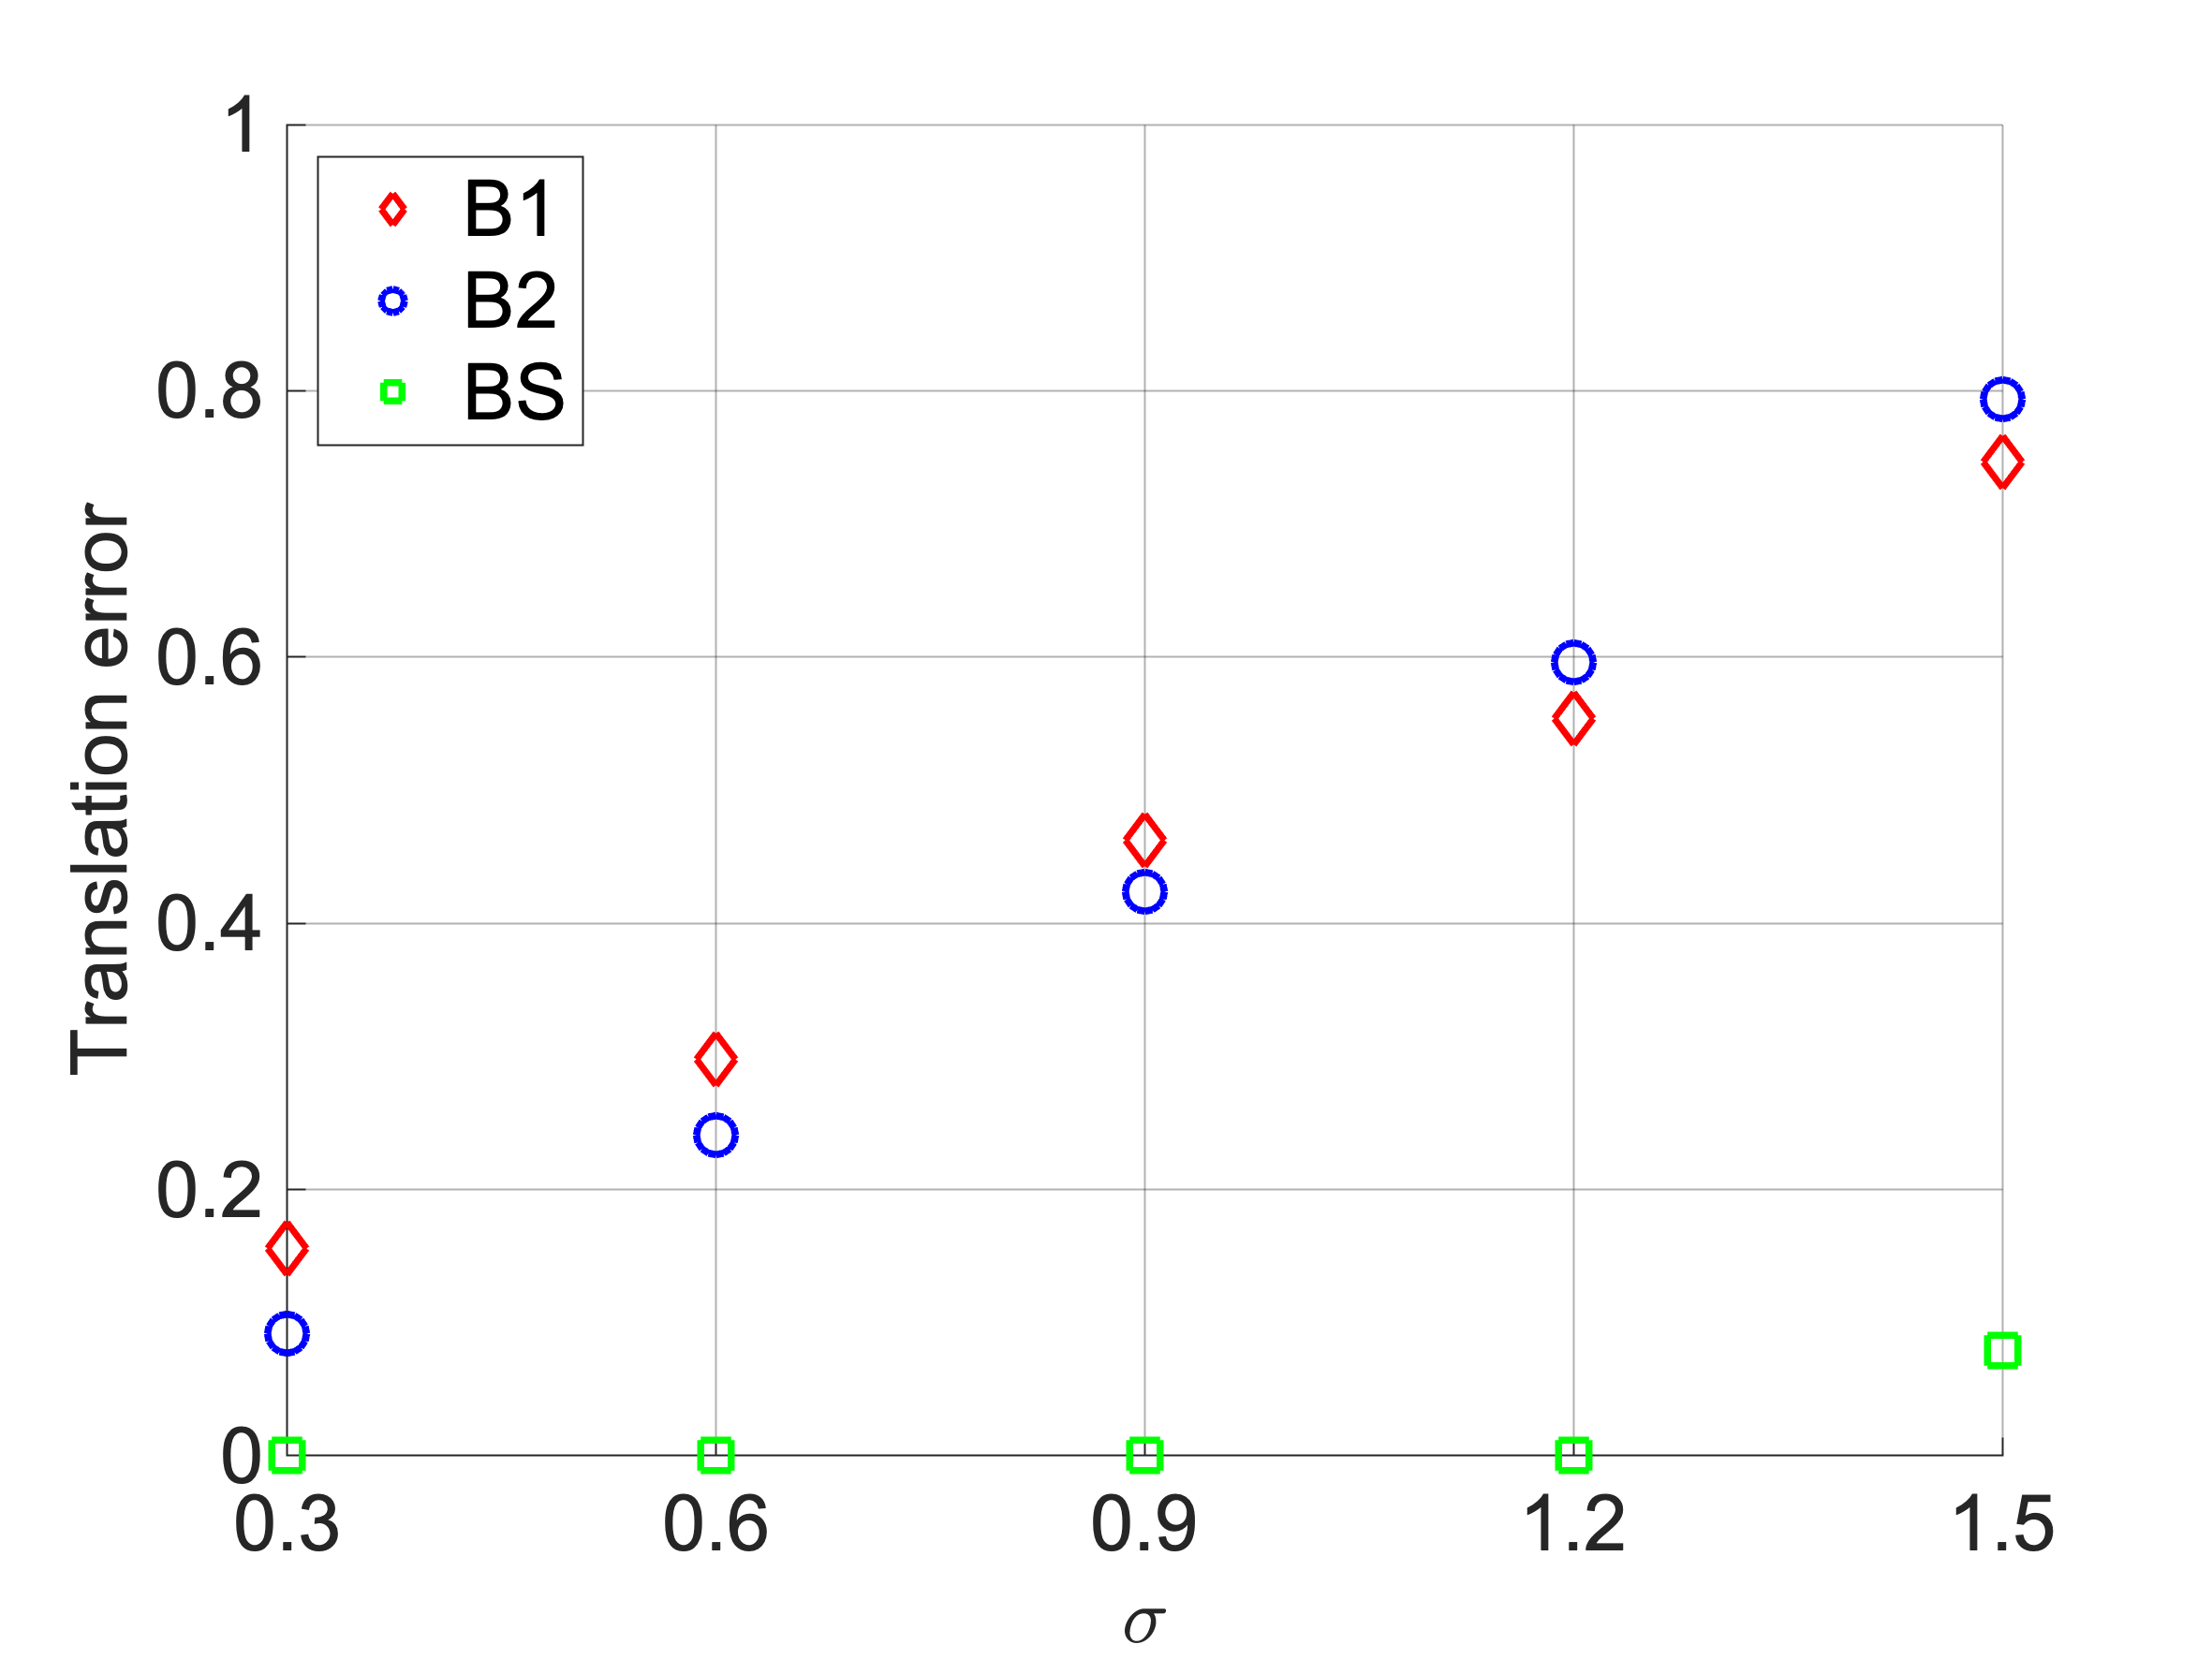
\includegraphics[width=0.22\linewidth]{figures/poster/res_1_t.png}&
 	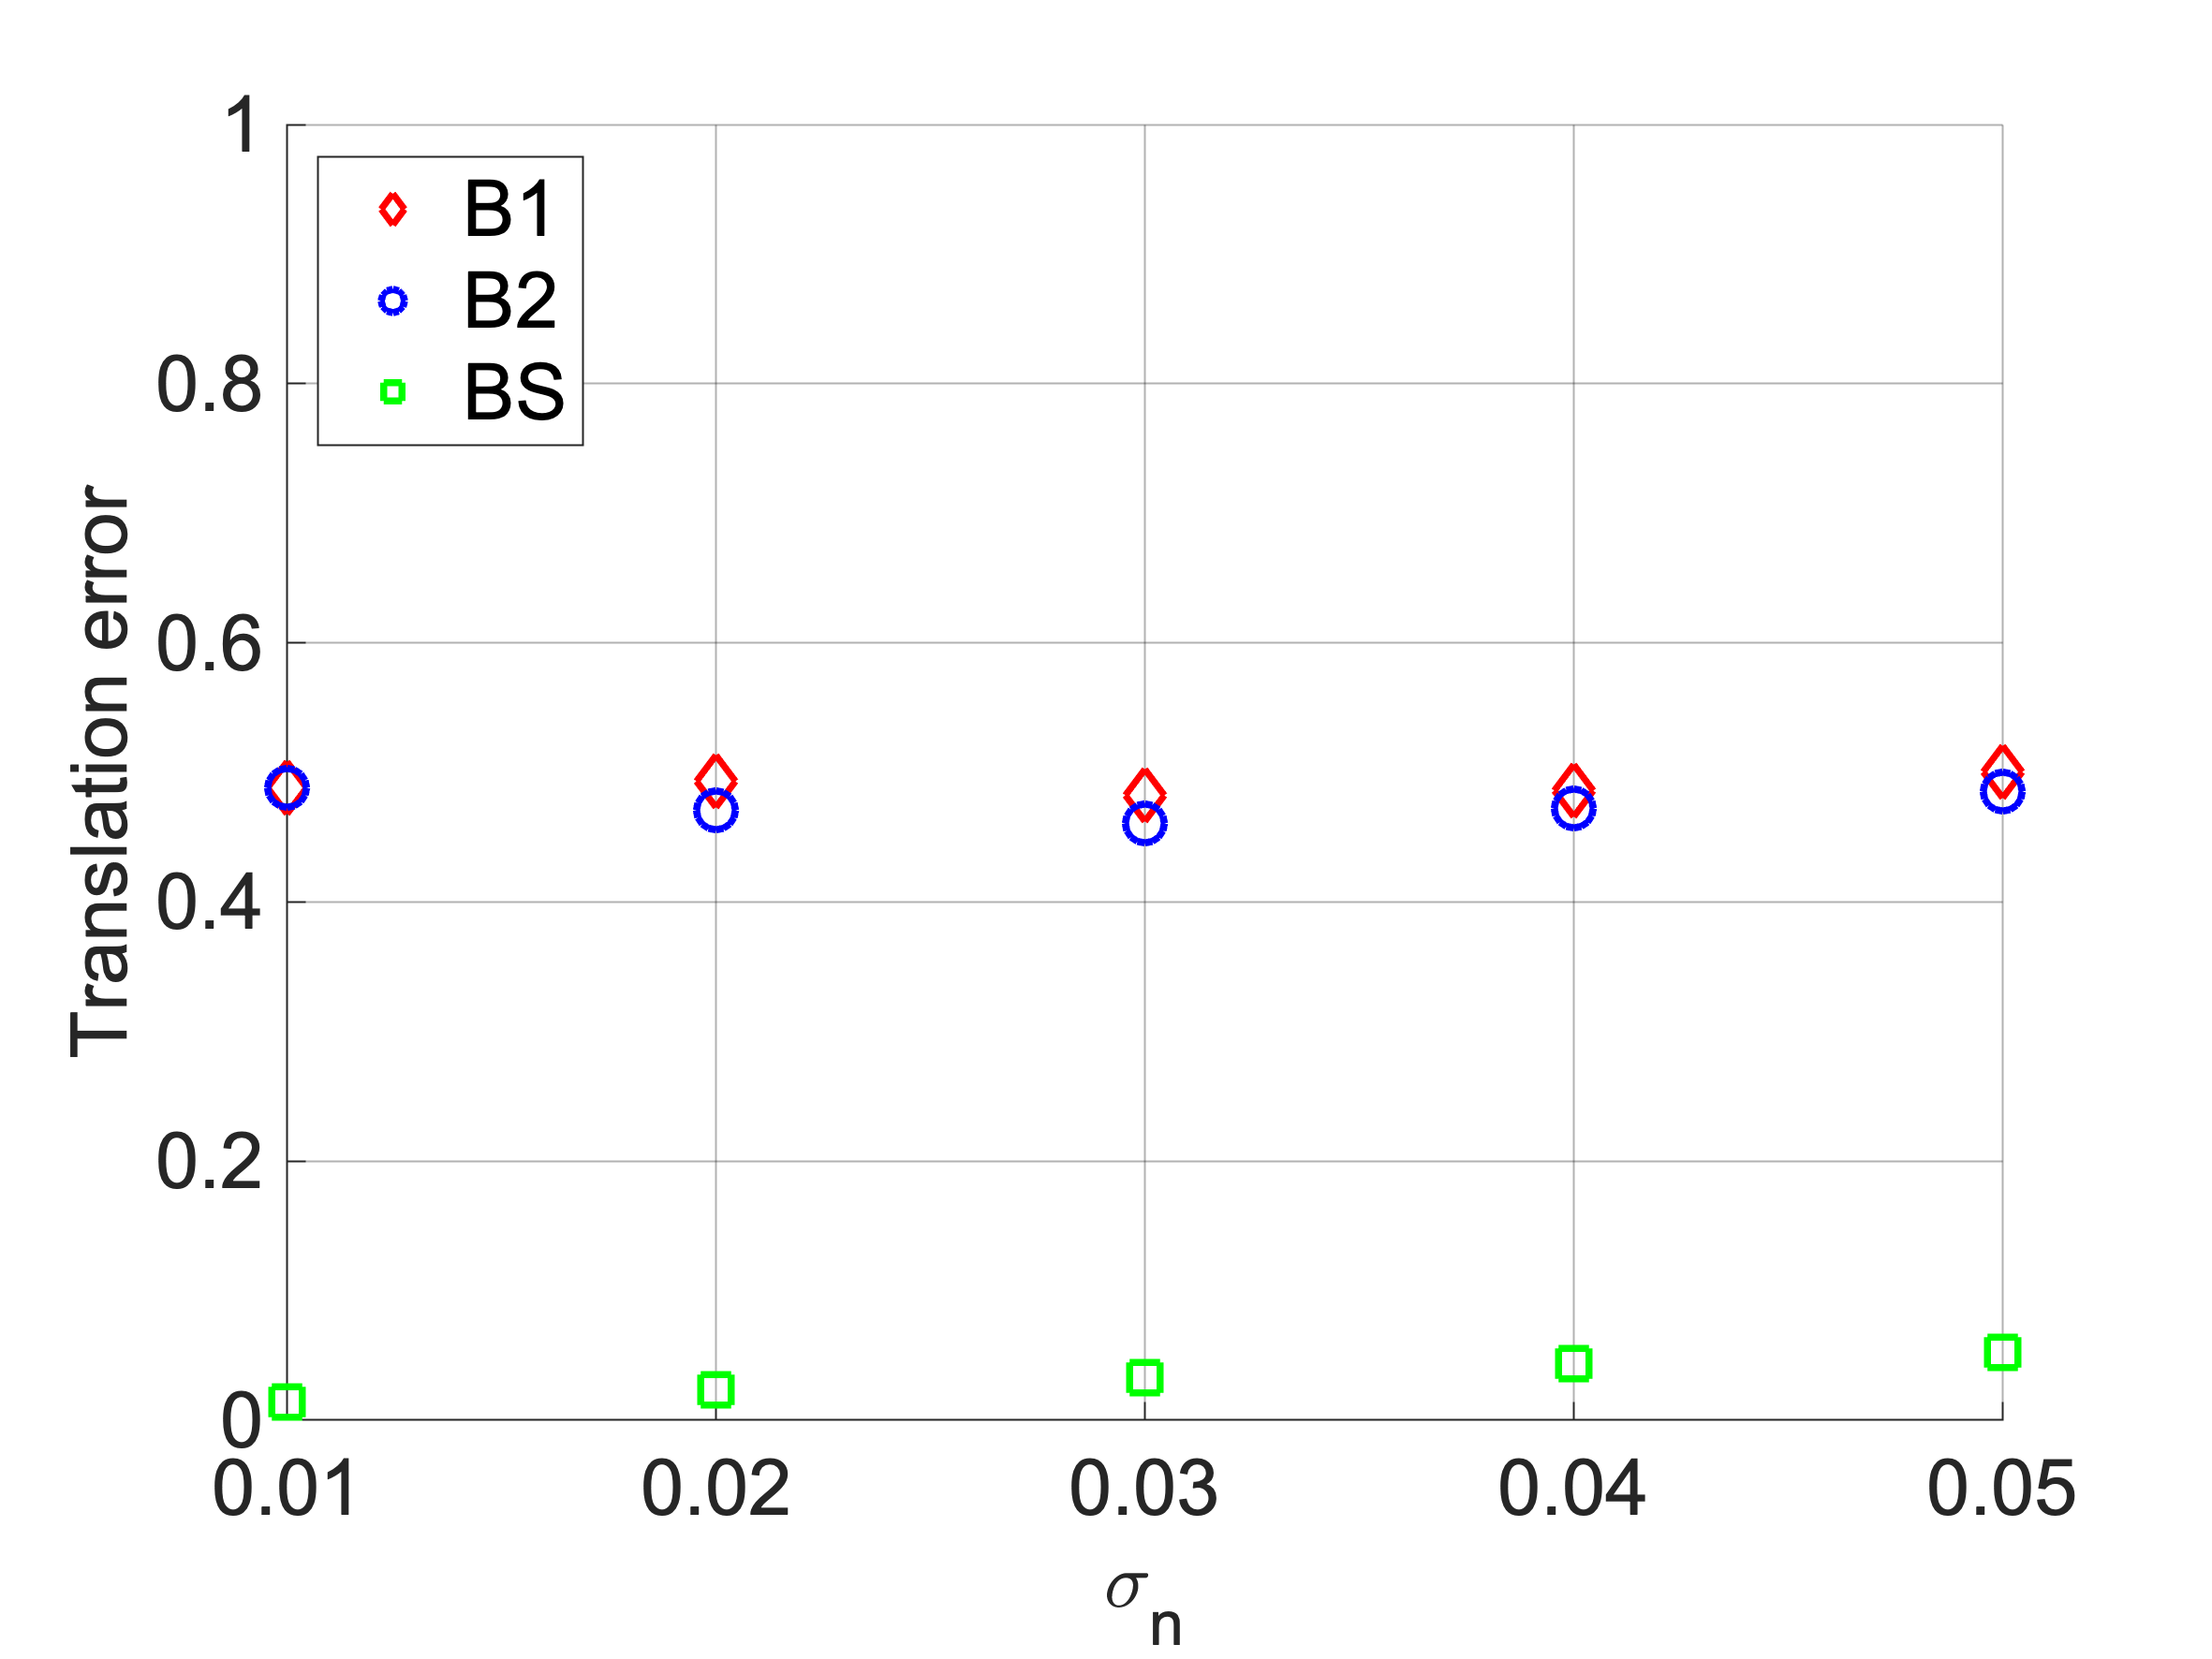
\includegraphics[width=0.22\linewidth]{figures/poster/res_3_t.png}&
 	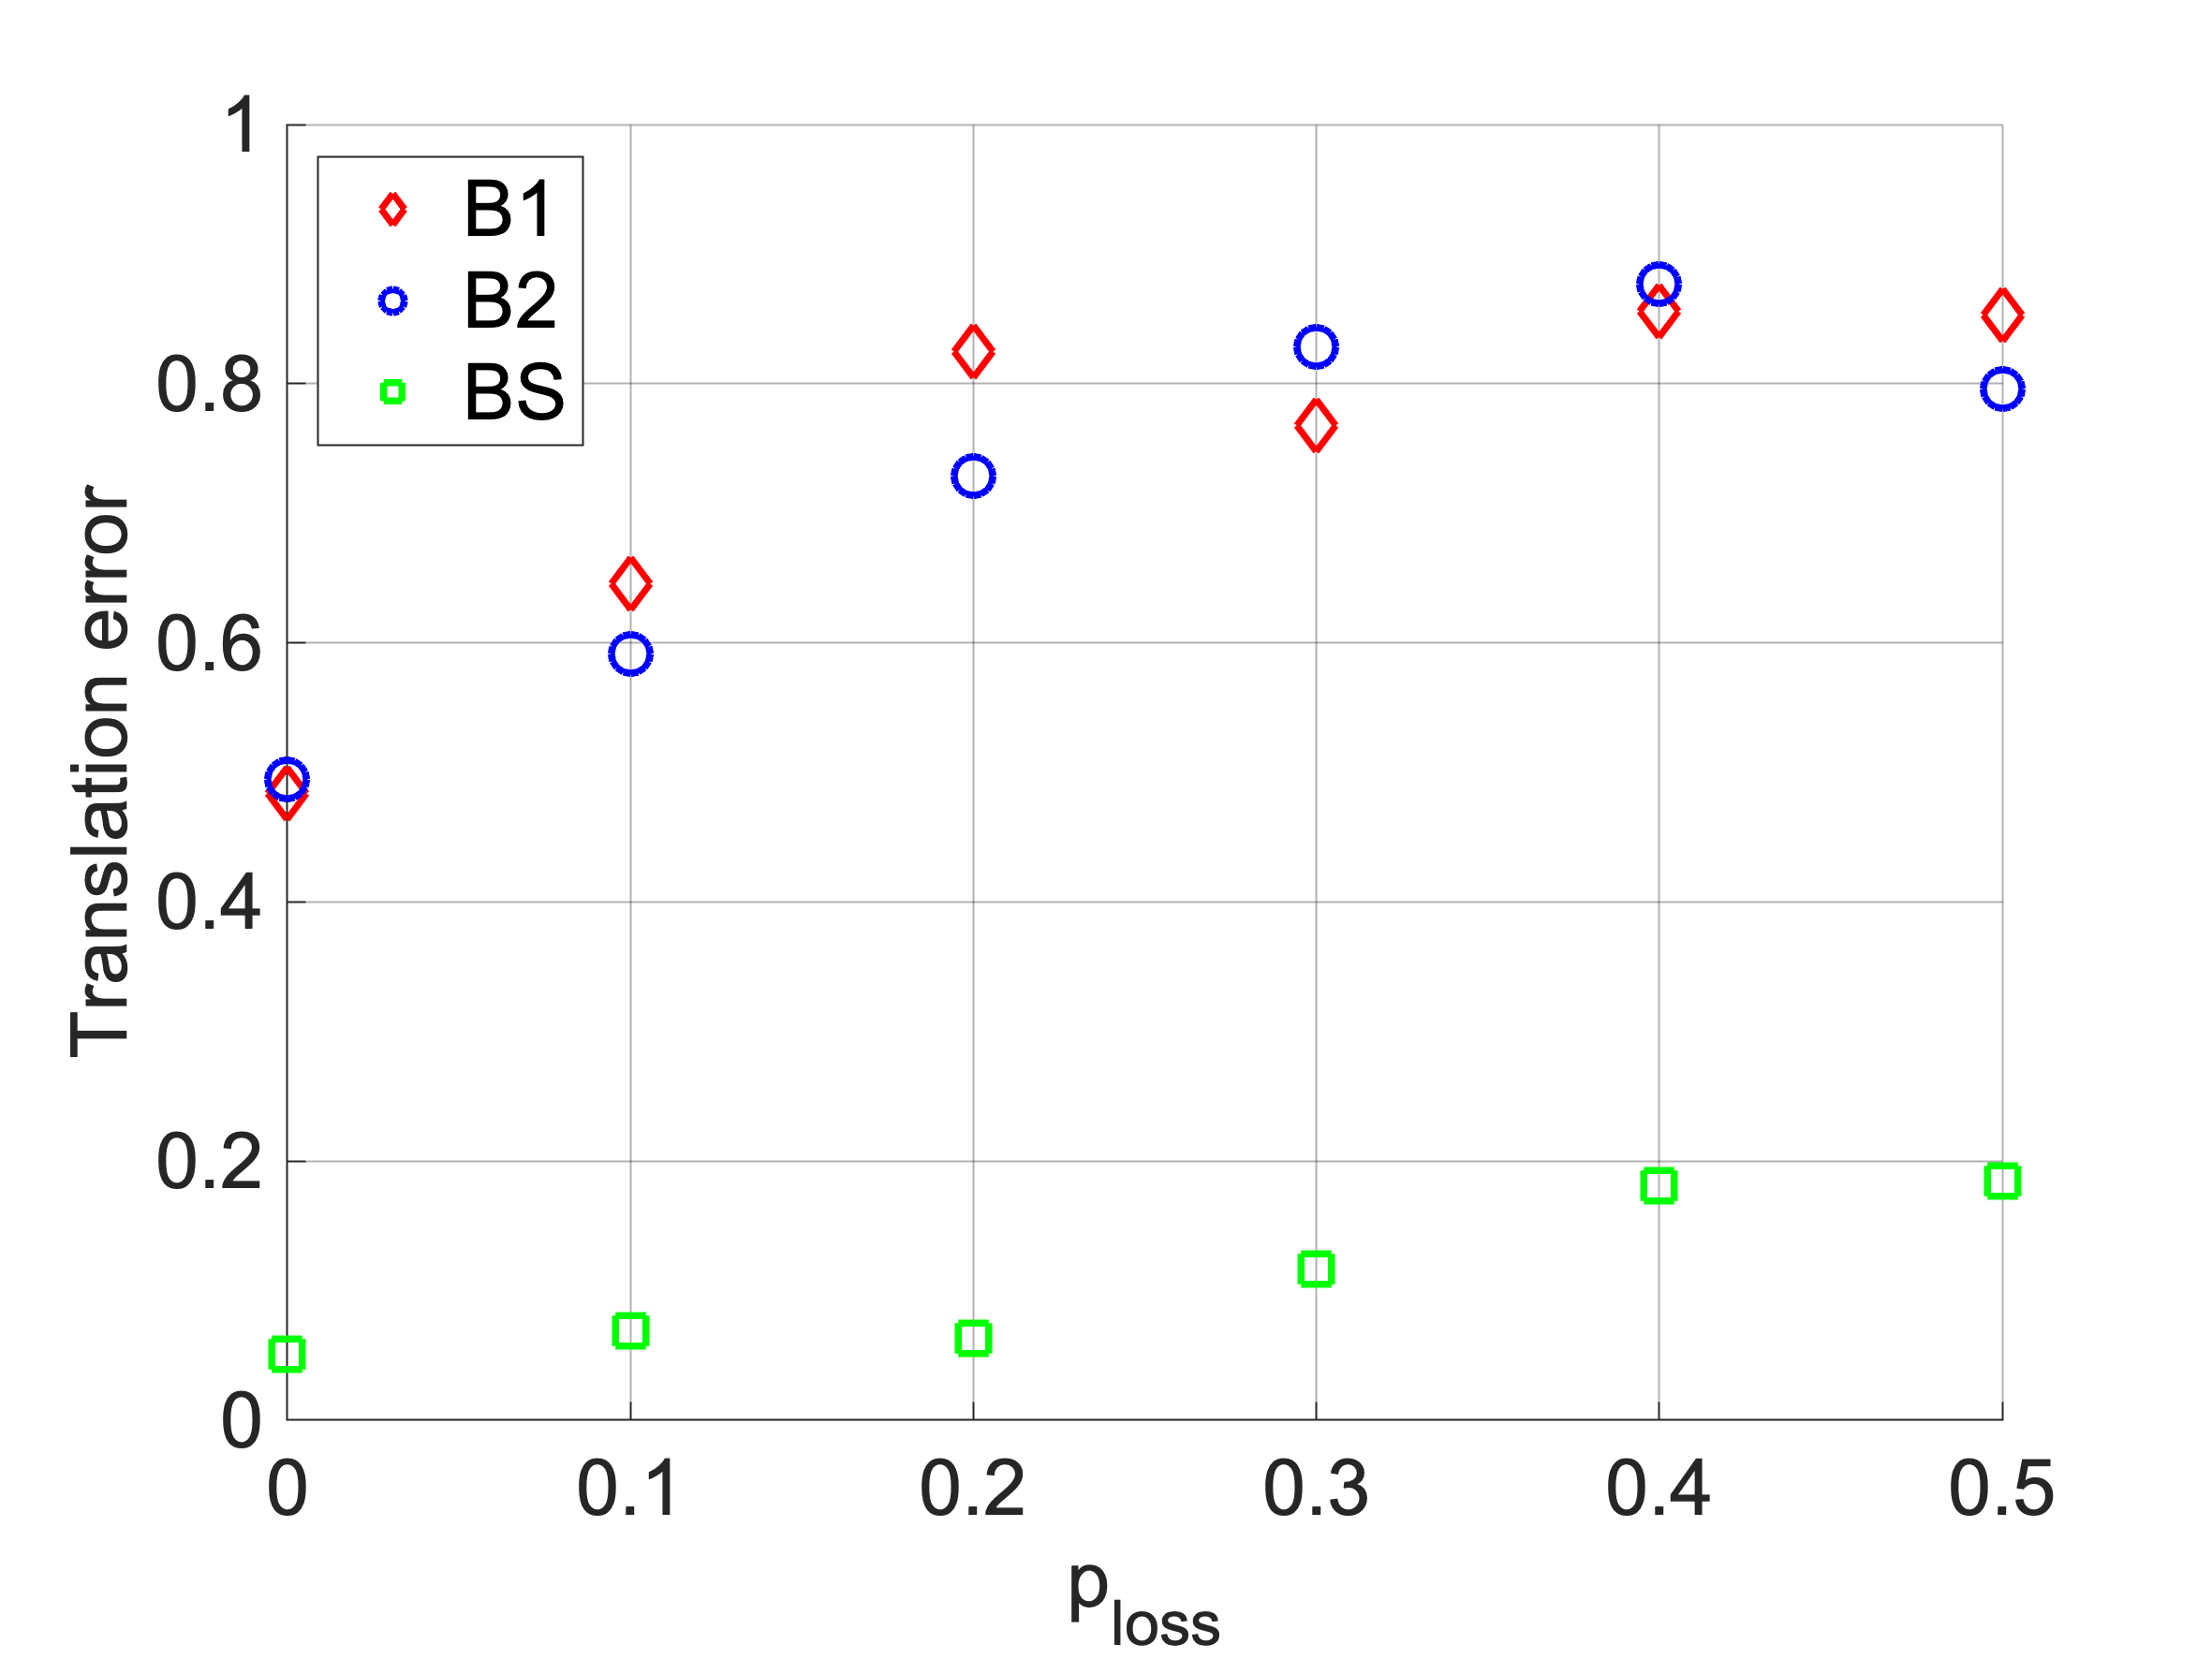
\includegraphics[width=0.22\linewidth]{figures/poster/res_4_t.png} &
 	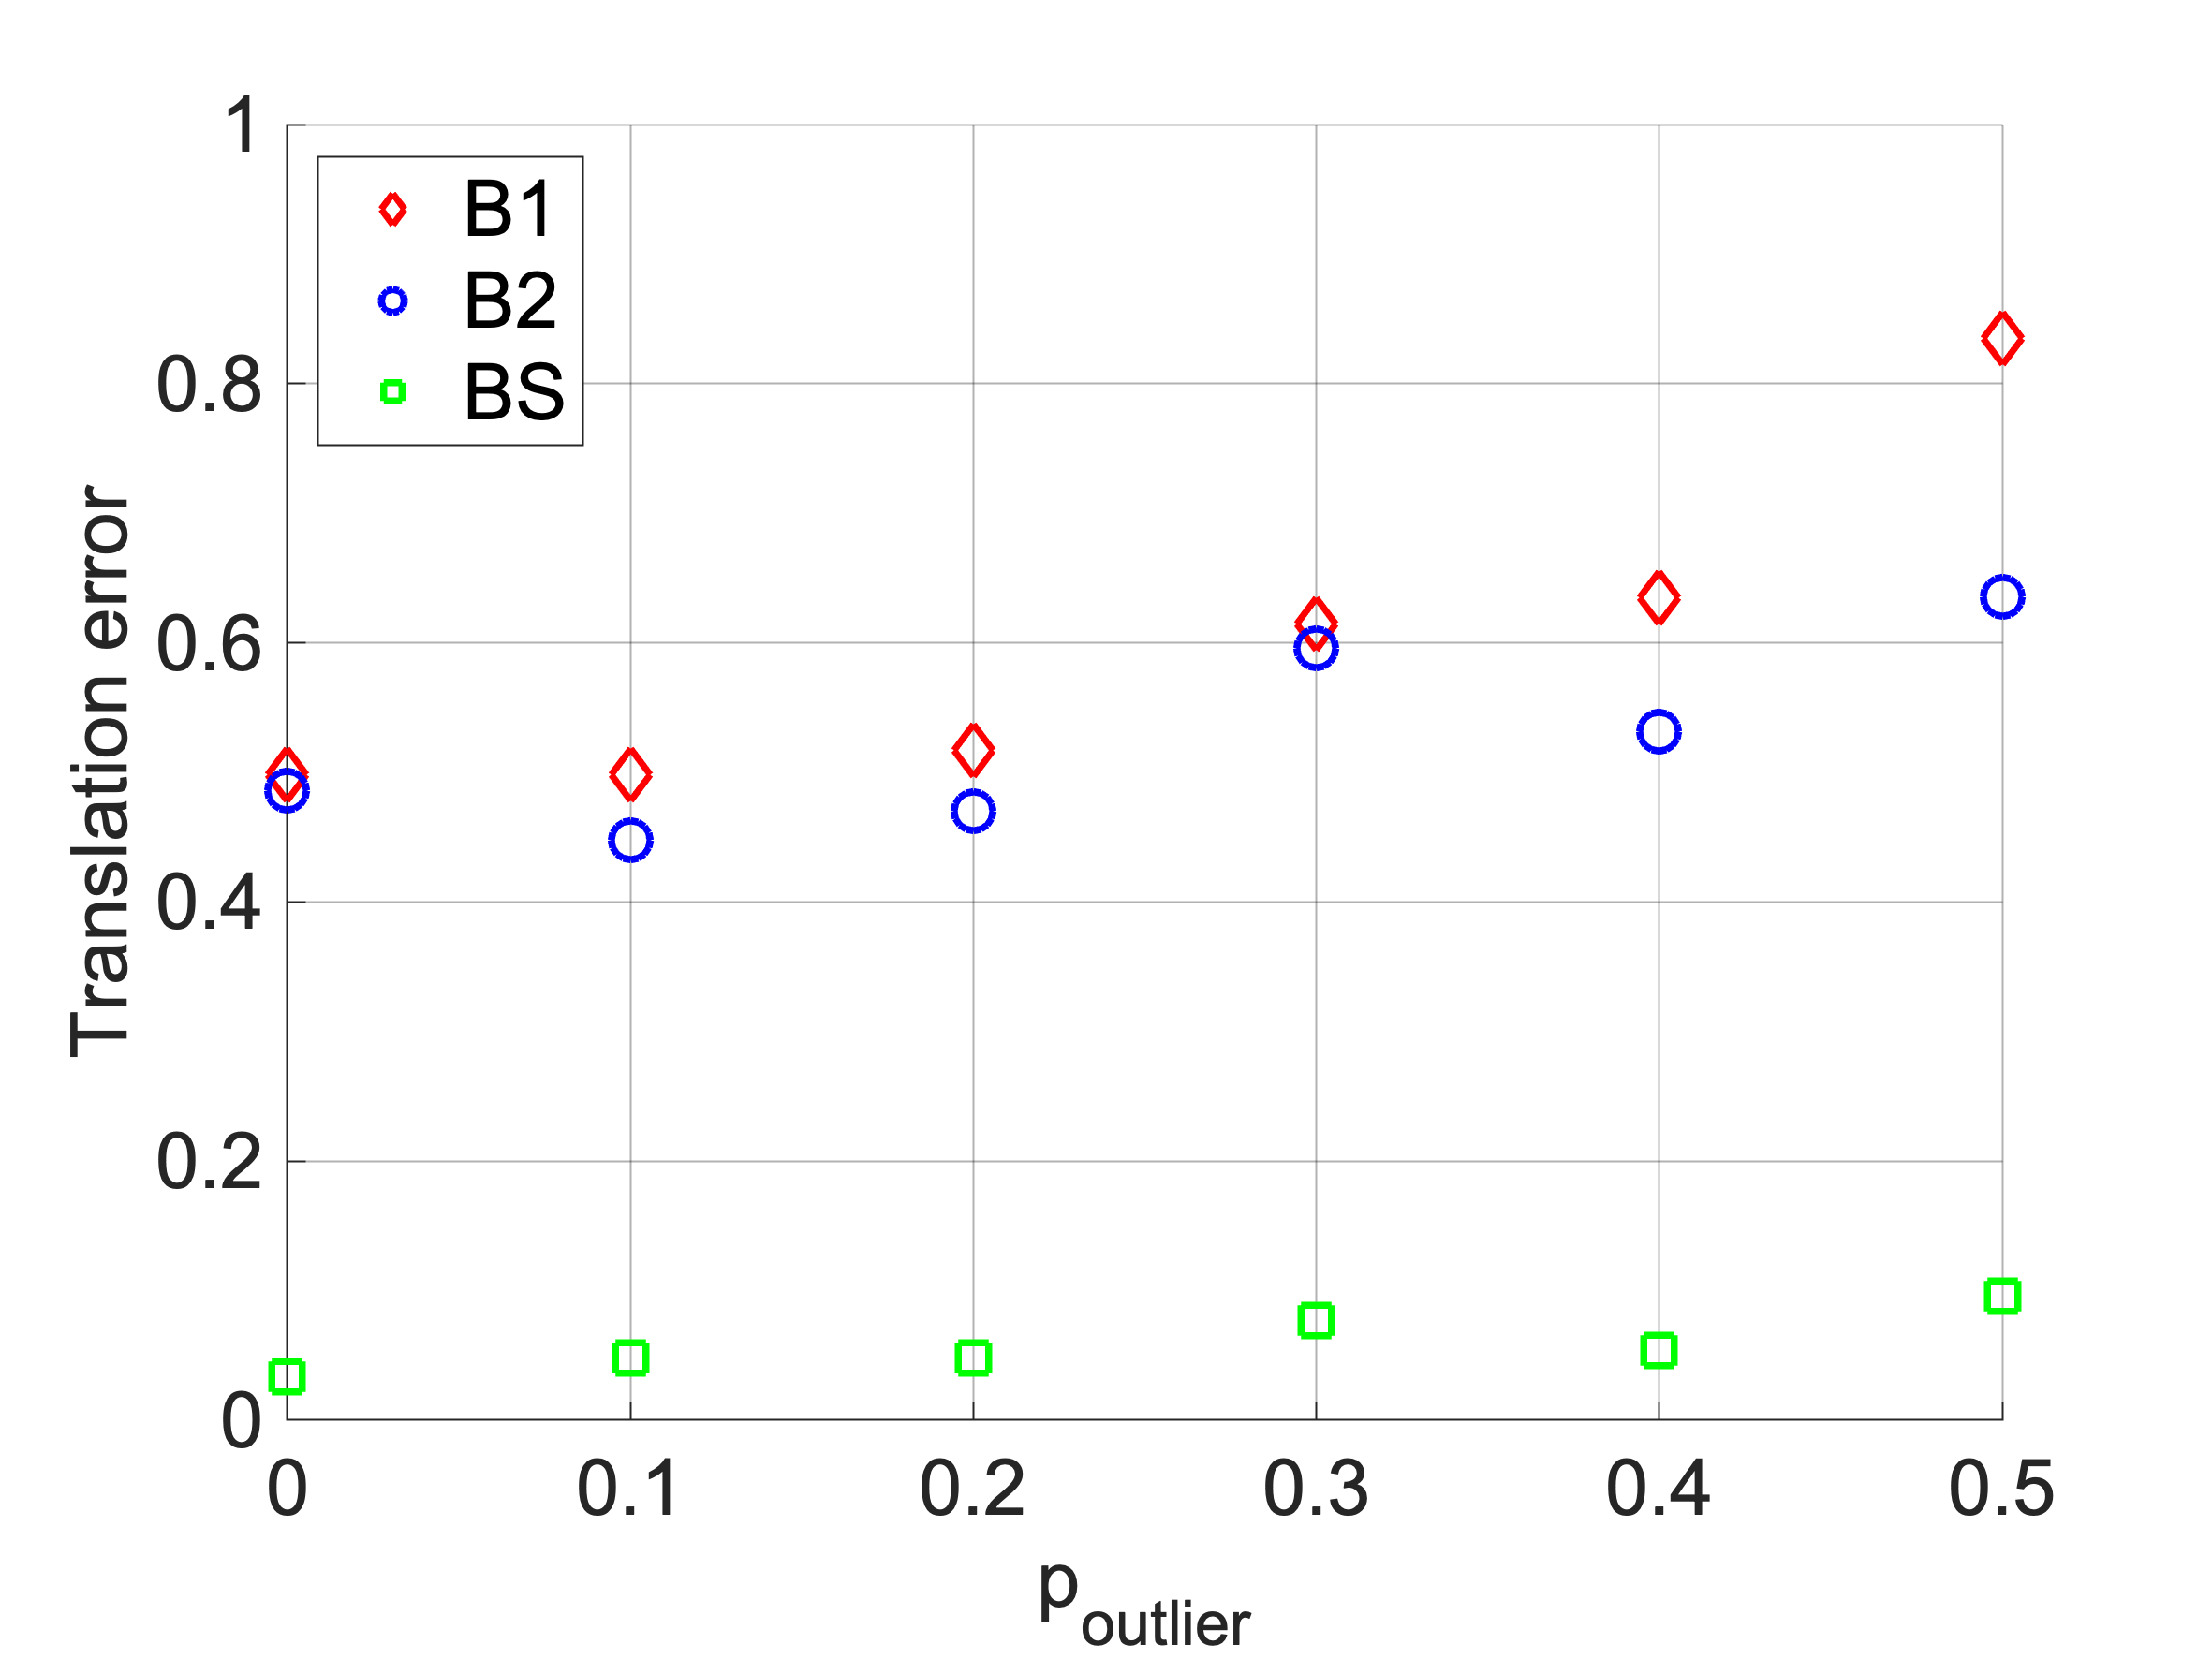
\includegraphics[width=0.22\linewidth]{figures/poster/res_5_t.png}\\[-0.1em]
 \end{tabular}  	  	
   }
 %%%%%%%%%%%%%%%%%%%%%%%%%%%%%%%%%%%%%%%%%%%%%%%%%%%%%%%%%%%%%%%%%%%%%%%%%%%%%%%
\headerbox{ML\&Fairness}{name=references,column=2,span=2,above=bottom}{
	%%%%%%%%%%%%%%%%%%%%%%%%%%%%%%%%%%%%%%%%%%%%%%%%%%%%%%%%%%%%%%%%%%%%%%%%%%%%%%
	\smaller
	Machine learning will be applied in this project for object detection, tracking, pose estimation. Learning based pose estimation is still very controversial, especially compared with traditional geometry based solutions where the underlying mathematics are known explicitly. In this case, bias existed in the data may result in biased pose estimation. \textbf{Fairness} could be helpful to design unbiased pose estimation netwrok.

} 
\end{poster}%
%
\end{document}
